% 预印本完整版论文主文件：基于 acmart (sigconf, nonacm) 模板构建，适用于 arXiv 上传
% 注意：acmart 已内置加载 newtxmath、xcolor 与 hyperref，请勿重复加载 amssymb 以免 \Bbbk 冲突

\documentclass[sigconf, nonacm, balance=false]{acmart}

\usepackage{amsmath,amsthm}
\usepackage{booktabs,array,multirow,tabularx}
\usepackage{algorithm}
\usepackage{algpseudocode}
\usepackage{subcaption}
\usepackage{microtype}

% 定理、引理、命题与定义环境
\newtheorem{theorem}{Theorem}
\newtheorem{proposition}[theorem]{Proposition}
\newtheorem{lemma}[theorem]{Lemma}
\newtheorem{corollary}[theorem]{Corollary}
\theoremstyle{definition}
\newtheorem{definition}{Definition}

% 排版容差控制，防止双栏窄行公式或长术语溢出
\tolerance=1500
\emergencystretch=2em
\widowpenalty=10000
\clubpenalty=10000
\graphicspath{{figures/}}

% 版本编译开关：
% 1. \preprinttrue 生成带完整数学推导与补充分析附录的本地/arXiv预印本版本；
%    投稿严格无附录的 PVLDB 正文版本时，只需改为 \preprintfalse 即可一键剥离附录及所有附录引用。
\newif\ifpreprint
\preprinttrue

% 2. 待填实验单元格宏：遵循学术成稿规范使用标准破折号占位，待云端外部基线跑完后直接填入实测数值
\newcommand{\emptycell}{\textemdash}

% 常用数学符号与系统名称宏定义
\newcommand{\rquiver}{Pelorus}
\newcommand{\pelorus}{Pelorus}
\newcommand{\quiver}{QuIVer}
\newcommand{\Bball}{\mathbb{B}_c^D}
\newcommand{\Bunit}{\mathbb{B}_1^D}
\newcommand{\Lmod}{\mathbb{L}_c^D}
\newcommand{\Sunit}{\mathbb{S}^{D-1}}
\newcommand{\R}{\mathbb{R}}
\newcommand{\E}{\mathbb{E}}
\newcommand{\Var}{\operatorname{Var}}
\newcommand{\Cov}{\operatorname{Cov}}
\newcommand{\MNR}{\mathrm{MNR}}
\newcommand{\sgn}{\operatorname{sgn}}
\newcommand{\arccosh}{\operatorname{arccosh}}
\newcommand{\atanh}{\operatorname{atanh}}
\newcommand{\asinh}{\operatorname{asinh}}
\newcommand{\popcnt}{\operatorname{popcnt}}
\newcommand{\missing}{\textemdash}
\DeclareMathOperator*{\argmin}{arg\,min}
\DeclareMathOperator*{\argmax}{arg\,max}

% 开源代码与实验工件仓库地址
\newcommand\codeavailabilityurl{https://github.com/Astrmira/Pelorus}

\begin{document}

\title[Pelorus: Warped-Product Graph Indexing for Hyperbolic Vector Search]{Pelorus: Warped-Product Graph Indexing for Hyperbolic Vector Search}

% 作者与单位信息（双盲投稿编译时可注释作者块并启用 Anonymous Author(s)）
\author{Wenxuan Xiao}
\affiliation{%
  \institution{Astrmira Tech.}
  \country{China}
}
\email{w.xiao@astrmira.com}

\author{Xu Cao}
\affiliation{%
  \institution{Astrmira Tech.}
  \country{China}
}
\email{x.cao@astrmira.com}

\begin{abstract}
Million-scale nearest-neighbor search in hyperbolic space must preserve geodesic order across radial shells while limiting the data fetched at each graph hop. An interior hub can occlude same-shell neighbors during graph construction, and the conformal distance factor amplifies directional error near the boundary.

We present \textbf{\rquiver{}}, a static proximity-graph index for the Poincar\'e ball and Lorentz hyperboloid. It separates radial scalars from two-bit spherical direction codes. QuadriPrune reserves edges for same-shell, inward and outward travel as well as geodesic neighbors. Queries read a compact header before fetching directional bitplanes, then rerank a short list using a separately stored vector representation. For tight boundary clusters, a purity-gated dictionary reuses the directional bits to encode tangent residuals.

On native {MERU-1M}, \rquiver{} serves $2{,}547$ and $53{,}483$ queries per second at $99.25\%$ Recall@10 on one and 24 threads. These rates are $1.97\times$ and $3.37\times$ the throughput of {HyperspaceDB} FP32 flat at $99.03\%$ recall. On mapped {Cohere-1M}, construction takes $35.0$ seconds versus $197.7$ for {Polar-FP32}. Hot navigation occupies $517$ versus $3{,}373$\,MB. Including the in-memory rerank vectors brings the respective index totals to $3{,}589$ and $3{,}373$\,MB. On {MERU-1M} at 24 threads with a $512$\,MiB SSD cache, switching the cold store from Cartesian FP32 to Cartesian FP16 reduces backend bytes read per query from $671$ to $358$\,KiB at over $99.9\%$ recall. On deep native {HyperE WordNet}, the fastest graph configurations meeting the $90\%$ recall target score $5{,}374$ cold vectors per query without the residual dictionary and $2{,}777$ with it, attaining $93.55\%$ and $93.09\%$ recall, respectively.

\end{abstract}

\maketitle

% 预印本页眉页脚样式与开源代码说明（已移除 PVLDB 引用格式、Endowment 版权页脚与刊物标识符）
\pagestyle{plain}
\vspace{.3cm}
\begingroup\small\noindent\raggedright\textbf{Code \& Artifact Availability:}\\
The source code, data, and/or other artifacts are available at \url{\codeavailabilityurl}.
\endgroup

% 正文各章节模块化引入
% 第一章：引言——从双曲检索系统瓶颈出发，阐明曲率流形下二比特量化与单度量构图的三大本质矛盾、核心洞察及贡献
\section{Introduction}
\label{sec:intro}

Representation models that embed text, images, and structured entities into negatively curved {Riemannian} manifolds---specifically the {Poincar\'e} ball $\Bball$ and the {Lorentz} hyperboloid $\Lmod$---provide a principled geometric inductive bias for hierarchical retrieval.
Because geodesic ball volume in hyperbolic space grows exponentially with radius rather than polynomially, trees, ontologies, and asymmetric entailment cones embed with far lower metric distortion than in flat {Euclidean} space~\cite{nickel2017poincare,sala2018representation,ganea2018entailment,gu2019mixed}.
Recent encoders scale curved representations across graph neural networks~\cite{nickel2018lorentz,chami2019hgcn}, fully hyperbolic Transformers and vision backbones~\cite{chen2022fully,khrulkov2020hyperbolic,ermolov2022hyperbolic}, million-vector multimodal alignment ({MERU}~\cite{desai2023meru}), and hyperbolic dense retrieval for retrieval-augmented generation ({HypRAG}~\cite{madhu2026hyprag,lewis2020rag}).

Serving low-latency, high-recall approximate nearest neighbor ({ANN}) queries over curved manifolds nevertheless remains a severe database systems bottleneck.
In flat {Euclidean} and cosine spaces, proximity graphs such as {HNSW}~\cite{malkov2020hnsw}, {NSG}~\cite{fu2019nsg}, and {Vamana} ({DiskANN})~\cite{subramanya2019diskann,azizi2025graph} define the latency--recall frontier.
Industrial and academic compressed graph engines---including locally-adaptive scalar quantization ({LVQ})~\cite{aguerrebere2023similarity}, binary lookup tables ({BBQ})~\cite{trent2024bbq}, randomized extended codes ({SymphonyQG})~\cite{gou2025symphonyqg}, and training-free 2-bit Sign-Magnitude ({SM}) indexing in {\quiver}~\cite{xiao2026quiver}---further accelerate search by reading full FP32 vectors only during tail reranking.
Hyperbolic locality-sensitive hashing~\cite{deng2026hyperboliclsh} and origin-tangent candidate retrieval~\cite{deng2026hyem} offer alternatives to building a curved graph. The origin log-map preserves distances from its center, but neighbor order for an off-center query can change. This distinction matters across datasets. On shallow native {MERU-1M}, tangent-space $L_2$ HNSW reaches $99.06\%$ recall, while on mapped {Cohere-1M} the same control peaks at $86.42\%$ (\S\ref{subsec:eval_external}).
Native hyperbolic graph indices~\cite{boytsov2013engineering,prokhorenkova2022hyperbolic,glukhota2026hyperspacedb} can use full coordinates or quantize ambient coordinates. A full-vector hop at $D=768$ reads $3{,}072$ bytes. Near the ball boundary the factor $2/(1-c\|x\|^2)$ also makes distance ordering sensitive to coordinate precision. These costs motivate separating the representation used for navigation from the vectors fetched for reranking.

\subsection{Why Flat Graph Indexing Breaks Under Negative Curvature}
\label{subsec:intro_obstructions}

How should proximity-graph indexes be architected for negatively curved manifolds?
Geometrically, $\Bball$ is not an isotropic vector space but a \emph{warped product} $\R_{\ge 0} \times_{\frac{1}{\sqrt{c}}\sinh(\sqrt{c}R)} \Sunit$ coupling a radial depth half-line with an exponentially expanding sphere.
Our theoretical and diagnostic study reveals that directly applying flat single-metric {Vamana} pruning~\cite{subramanya2019diskann} or flat compressed navigation~\cite{aguerrebere2023similarity,gao2024rabitq,xiao2026quiver} on this warped product can incur three geometric errors:

\begin{enumerate}
  \item \textbf{Cross-Shell Conformal Non-Cancellation and Lorentz-MIPS Blowup.}
  In flat cosine search, ranking candidates $x$ and $y$ against query $q$ evaluates $\langle u_q, u_x\rangle - \langle u_q, u_y\rangle$; because both terms weight $u_q$ equally, first-order quantization noise on $u_q$ cancels identically as $u_x \to u_y$~\cite{xiao2026decisions}.
  In $\Bball$, the monotonic geodesic proxy weights each directional inner product $\langle u_q, u_v\rangle$ by a candidate-dependent conformal factor $W(r_q, r_v) = 2 r_q r_v f_q f_v = \frac{2}{c}\sinh\rho_q\sinh\rho_v$.
  Whenever $r_x \ne r_y$, query quantization leaves an uncancelled residual scaled by $W(r_q, r_y) - W(r_q, r_x) \ne 0$ that grows exponentially with boundary depth.
  Worse, quantizing $(D+1)$-dimensional {Lorentz} coordinates directly via Minkowski inner products multiplies coordinate quantization noise by $\|\tilde{z}\|_2 = \Theta(e^\rho)$ without separating radial norms.

  \item \textbf{Radial Occlusion Bounds and Angular Escape Conditions.}
  An interior neighbor $p$ with $R_p<R_u/\alpha$ in {Vamana} pruning~\cite{subramanya2019diskann} occludes every candidate inside $R_v\le(R_u-\alpha R_p)/(\alpha+1)$ by the triangle inequality. For two vertices on the same shell of depth $\rho$, an origin neighbor leaves an angular cone with $\sin(\theta_{uv}/2)<\sinh(\alpha\rho/2)/\sinh\rho$. At $\alpha=1.2$ its half-angle falls from $73.7^\circ$ in the flat limit to $23.1^\circ$ at $\rho=4$.
  These bounds motivate reserving angular links. We measure the effect of removing each pruning channel on {Cohere-1M} (\S\ref{subsec:eval_ablation}).

  \item \textbf{Boundary Cluster Margins and Fixed-Budget Pool Dilution.}
  For equal-depth candidates in a tight cone, the ranking margin scales as $\beta_{q,c}\beta_v$ times the tangent-direction difference. Global-code comparison error depends on the covariance between the candidate errors (Theorem~\ref{thm:tangent_cone}).
  As the comparison margin-to-noise ratio ({$\MNR$}) collapses toward zero, expanding beam width $L$ under a fixed rerank budget $B$ counterintuitively \emph{reduces} recall by flooding the candidate pool with indistinguishable intra-cluster distractors: on a 128-query trace from the 1M-vector clustered narrow-shell benchmark, beam traversal visits $93.9\%$ of true top-$10$ neighbors at $L=256$ yet retains only $49.3\%$ in the finalist beam and $33.0\%$ after pool gating ($34.2\%$ across all $2{,}000$ queries), and raising $L$ from $256$ to $2{,}048$ lowers recall monotonically from $34.2\%$ to $27.8\%$.
  Local tangent encoding allocates the existing bitplanes to normalized within-cone variation, retaining native coordinates outside the selected cones.
\end{enumerate}

\subsection{Warped-Product Polar Co-Design in \rquiver{}}
\label{subsec:intro_solution}

We address these obstructions with \textbf{\rquiver{}}---named after the maritime bearing dial that decouples angular direction from radial course---an in-memory hyperbolic proximity-graph index grounded in \emph{warped-product polar decoupling}.
Every point $x \in \Bball$ (and via exact stereographic isometry every point $z \in \Lmod$) is factored into unquantized FP32 radial scalars $(r_x,F_x,\rho_x)$, with $F_x=f_x/2$, stored in a 32-byte header and a scale-invariant directional code on the unit sphere $\Sunit$, instantiated via training-free 2-bit {SM} bitplanes.
Storing radial scalars independently in FP32 keeps directional-code error out of the conformal denominator $1-cr_x^2$ and decouples hyperbolic distance into scalar radial lower bounds plus weighted spherical inner products.

From this representation, \rquiver{} co-designs conformal polar estimation primitives, fiber-bundle topology, and page-aligned hardware execution:
\begin{itemize}
  \item \emph{Conformal Polar Estimation and Tangent-Cone Recovery (\S\ref{sec:theory}):}
  We prove that polar decoupling makes same-shell directional flip criteria invariant to query boundary proximity ($f_q \to \infty$), derive a deterministic zero-parameter \emph{orthogonal-projection asymmetric estimator} (\textsc{Stage-0.5}) based on exact two-level {SM} Pythagorean reconstruction, establish $1$-strong convexity of the hyperbolic-cosine objective and derive its closed-form \emph{radial minimizer} along directional rays, and introduce a purity-gated \emph{local tangent-cone residual code} paired with an off-axis \emph{Conformal Jacobian plateau gate} (\textsc{CJ-Gate}) that attenuates intra-cone tangent error with zero per-vertex byte overhead while keeping diffuse embeddings on the zero-overhead global path.

  \item \emph{Warped-Product Fiber-Bundle Topology (\S\ref{sec:design}):}
  Rather than pruning edges under a single isotropic predicate, \rquiver{} inserts vertices inside-out by geodesic depth and partitions each out-degree list across four geometric channels via \emph{QuadriPrune}: stem-excess geodesic fibers, radially shielded \emph{isobathic} (same-shell) rings that restrict angular domination to nearby depths, and step-aligned inward and outward radial elevators, followed by a degree-preserving spanning-tree chord-swap pass that achieves full directed {BFS} reachability from the entry hub on all 21 Core builds in the three-seed sweep.

  \item \emph{Page-Aligned Polar Execution (\S\ref{sec:system}):}
  To let header and bitplane reads share an address translation, \rquiver{} co-locates each vertex's $32$\,B polar header, binomial-variance-stabilized 256-bit early sketch, and complete 2-bit {SM} bitplanes inside a power-of-two record within a single $4096$\,B OS page ($16$ vertices/page at $D=768$), evaluates surviving 5-popcount bitplane products via a 3-to-2 carry-save {AVX2} kernel, refines the converged beam in L1 cache via fixed-point masked subset sums, and reranks the top tail in IEEE-754 FP64 {SIMD}.
\end{itemize}

\paragraph{Contributions.}
Our main contributions are summarized as follows:
\begin{itemize}
  \item Building on flat comparison-decision theory~\cite{xiao2026decisions}, we analyze conformal polar quantization and hyperbolic {Vamana} pathologies on $\Bball$ and $\Lmod$, characterizing query boundary-depth invariance, cross-shell query-noise non-cancellation, Lorentz-MIPS quantization blowup, radial occlusion with exponential angular-cone contraction, fixed-budget pool dilution, deterministic orthogonal-projection de-biasing, and purity-gated zero-byte-per-node tangent-cone {$\MNR$} recovery (\S\ref{sec:theory}).
  \item We design a warped-product graph construction and routing pipeline combining inside-out geodesic seeding, stem-excess {QuadriPrune} degree partitioning, spanning-tree chord-swap island repair (full directed reachability on all 21 Core builds), and routing via the constrained radial minimizer (\S\ref{sec:design}).
  \item We engineer a stateless hardware-conscious execution engine integrating $4096$\,B single-page vertex co-location, variance-stabilized 256-bit beam filtering, 3-to-2 carry-save {AVX2} popcounts, L1-bounded \textsc{Stage-0.5}/\textsc{CJ-Gate} refinement, and FP64 {SIMD} geodesic reranking (\S\ref{sec:system}).
  \item On native {MERU-1M}, \rquiver{} serves $2{,}547$/$53{,}483$\,QPS at $99.25\%$ Recall@10 (1T/24T). On mapped {Cohere-1M}, construction takes $35.0$\,s on 32 threads, and at the $99\%$ recall target the index serves $4.23\times$/$6.06\times$ the 1T/24T throughput of {Polar-FP32} ($99.02\%$ and $99.27\%$ attained, respectively). Navigation uses $517$\,MB, with a further $3{,}072$\,MB for in-memory exact reranking. We measure the effects of compact pages and SSD-backed reranking separately, and trace how the native {MERU} and deep {WordNet} graphs respond to changes in pruning, routing and residual coding (\S\ref{sec:eval}).
\end{itemize}

% 第二章：预备知识与问题建模——翘曲乘积双曲几何、洛伦兹等距映射、二比特条件均值勾股恒等式与离散比较算子
\section{Preliminaries and Problem Formulation}
\label{sec:prelim}

We formalize hyperbolic metric models as warped-product manifolds, establish the exact polar geodesic proxy, characterize the two-level spherical Sign-Magnitude ({SM}) geometry, and define the discrete comparison decisions governing quantized graph construction and search.

\subsection{Hyperbolic Models and Warped-Product Unification}
\label{subsec:models}

\paragraph{{Poincar\'e} Ball and {Lorentz} Stereographic Isometry.}
For constant negative sectional curvature $-c < 0$, the $D$-dimensional {Poincar\'e} ball is the open manifold
\begin{equation}
  \Bball = \bigl\{x \in \R^D : c\|x\|_2^2 < 1\bigr\}, \qquad g_x^{\mathbb{B}} = f_x^2 I_D,
  \label{eq:poincare_manifold}
\end{equation}
with conformal metric factor $f_x = \frac{2}{1 - c\|x\|_2^2}$.
The Riemannian geodesic distance between $q, v \in \Bball$ is
\begin{equation}
  d_{\mathbb{B}}(q, v) = \frac{1}{\sqrt{c}}\arccosh\!\left(1 + \frac{2c\|q - v\|_2^2}{(1 - c\|q\|_2^2)(1 - c\|v\|_2^2)}\right).
  \label{eq:poincare_dist}
\end{equation}
Many modern hyperbolic encoders, including fully hyperbolic networks~\cite{chen2022fully}, {MERU}~\cite{desai2023meru}, and {HypRAG}~\cite{madhu2026hyprag}, parameterize embeddings on the upper sheet of the $(D+1)$-dimensional {Lorentz} hyperboloid
$\Lmod = \{z = (z_0, \tilde{z}) \in \R \times \R^D : -z_0^2 + \|\tilde{z}\|_2^2 = -1/c,\; z_0 > 0\}$
under $d_{\mathbb{L}}(z, z') = \frac{1}{\sqrt{c}}\arccosh\bigl(c(z_0 z'_0 - \langle \tilde{z}, \tilde{z}'\rangle)\bigr)$.
Stereographic projection $\Pi : \Lmod \to \Bball$,
\begin{equation}
  \Pi(z_0, \tilde{z}) = \frac{\tilde{z}}{1 + \sqrt{c}\,z_0},
  \label{eq:lorentz_isometry}
\end{equation}
is a global Riemannian isometry satisfying $d_{\mathbb{B}}(\Pi(z), \Pi(z')) = d_{\mathbb{L}}(z, z')$ for all $z, z' \in \Lmod$~\cite{nickel2018lorentz}\ifpreprint\ (proved algebraically in Appendix~\ref{app:warped_product})\fi.
Projecting $\Lmod$ embeddings via~\eqref{eq:lorentz_isometry} at ingestion eliminates the redundant time-like coordinate $z_0$ without losing exact geodesic distances or rankings; as shown in Theorem~\ref{thm:conformal_flip}(3), it also avoids exponential quantization error blowup on unbounded spatial norms $\|\tilde{z}\|_2$.

\paragraph{Warped-Product Decomposition and Order-Isomorphic Polar Proxy.}
Every $x \in \Bball$ decomposes into Euclidean radius $r_x = \|x\|_2 \in [0, 1/\sqrt{c})$ and unit spherical direction $u_x \in \Sunit$ ($u_0 = e_1$ at $r_x = 0$).
Let $R_x = d_{\mathbb{B}}(0, x)$ denote geodesic radius from the origin and $\rho_x = \sqrt{c}\,R_x = 2\atanh(\sqrt{c}\,r_x)$ denote dimensionless geodesic depth, which satisfy the exact identities $\sinh\rho_x = \sqrt{c}\,r_x f_x$ and $\cosh\rho_x = c r_x^2 f_x + 1 = f_x - 1$.
In coordinates $(R, u) \in (0, \infty) \times \Sunit$, $\Bball \setminus \{0\}$ is isometric to the warped-product manifold
\begin{equation}
  \begin{aligned}
    \Bball \setminus \{0\} &\cong (0, \infty) \times_{\frac{1}{\sqrt{c}}\sinh(\sqrt{c}R)} \Sunit, \\
    \mathrm{d}s^2 &= \mathrm{d}R^2 + \frac{1}{c}\sinh^2(\sqrt{c}R)\,\mathrm{d}\Omega_{D-1}^2,
  \end{aligned}
  \label{eq:warped_metric}
\end{equation}
where spherical fiber distances expand exponentially as $\frac{1}{\sqrt{c}}\sinh(\sqrt{c}R) = \frac{1}{2\sqrt{c}}e^{\rho}(1 - e^{-2\rho})$.
Expanding $\|q - v\|_2^2 = (r_q - r_v)^2 + 2 r_q r_v(1 - \gamma_{qv})$ for spherical cosine $\gamma_{qv} = \langle u_q, u_v\rangle = \cos\theta_{qv} \in [-1, 1]$ yields the \emph{polar geodesic proxy}:
\begin{equation}
  P_{\mathbb{B}}(q, v) \triangleq \|q - v\|_2^2 f_q f_v = R(r_q, r_v) + W(r_q, r_v)\bigl(1 - \gamma_{qv}\bigr),
  \label{eq:polar_proxy}
\end{equation}
where the radial discrepancy term and conformal angular weight are
\begin{equation}
  \begin{aligned}
    R(r_q, r_v) &= (r_q - r_v)^2 f_q f_v, \\
    W(r_q, r_v) &= 2 r_q r_v f_q f_v = \frac{2}{c}\sinh\rho_q \sinh\rho_v.
  \end{aligned}
  \label{eq:radial_conformal_weights}
\end{equation}
By the hyperbolic law of cosines, $\frac{c}{4}P_{\mathbb{B}}(q, v) = \sinh^2\!\bigl(\frac{\rho_q - \rho_v}{2}\bigr) + \sinh\rho_q\sinh\rho_v\sin^2\!\bigl(\frac{\theta_{qv}}{2}\bigr) = \sinh^2\!\bigl(\frac{\sqrt{c}}{2}d_{\mathbb{B}}(q, v)\bigr)$, so exact geodesic distance relates to $P_{\mathbb{B}}(q, v)$ through
\begin{equation}
  \begin{aligned}
    d_{\mathbb{B}}(q, v)
    &= \frac{1}{\sqrt{c}}\arccosh\!\left(1 + \frac{c}{2} P_{\mathbb{B}}(q, v)\right) \\
    &= \frac{2}{\sqrt{c}}\asinh\!\left(\frac{1}{2}\sqrt{c\,P_{\mathbb{B}}(q, v)}\right).
  \end{aligned}
  \label{eq:proxy_to_geodesic}
\end{equation}
Because $z \mapsto \frac{2}{\sqrt{c}}\asinh\bigl(\frac{1}{2}\sqrt{c z}\bigr)$ is strictly increasing on $[0, \infty)$, $P_{\mathbb{B}}(q, v)$ is strictly order-isomorphic to $d_{\mathbb{B}}(q, v)$, deferring transcendental evaluations to the final $k$ returned neighbors.
Furthermore, in the flat-curvature limit $c \to 0^+$, $f_x \to 2$ and $\frac{1}{4}P_{\mathbb{B}}(q, v) \to \|q - v\|_2^2$, recovering flat Euclidean and spherical geometry continuously.

\subsection{Exact Two-Level Spherical SM Geometry and Decision Operators}
\label{subsec:sm_decisions}

\paragraph{Deterministic Conditional-Mean Two-Level {SM} Reconstruction.}
In polar coordinates, $u_v \in \Sunit$ lies on the unit sphere independently of $r_v$.
Following {\quiver}~\cite{xiao2026quiver}, training-free 2-bit {SM} encodes each coordinate $u_{v,i}$ ($i \in \{1,\dots,D\}$) into two packed bitplanes:
a sign bit $s_{v,i} = \mathbb{I}[u_{v,i} \ge 0]$ and a strong-magnitude bit $m_{v,i} = \mathbb{I}[|u_{v,i}| > \tau_v]$ relative to the L1 mean threshold $\tau_v = \frac{1}{D}\sum_{j=1}^D |u_{v,j}|$, with strong-bit count $s_v = \sum_{i=1}^D m_{v,i}$.
Partitioning $\{1,\dots,D\}$ into weak indices $I_{0,v} = \{i : m_{v,i} = 0\}$ ($|I_{0,v}| = D - s_v$) and strong indices $I_{1,v} = \{i : m_{v,i} = 1\}$ ($|I_{1,v}| = s_v$) defines conditional magnitude means $a_v = \frac{1}{D - s_v}\sum_{i \in I_{0,v}} |u_{v,i}|$ ($0$ if $s_v = D$), $b_v = \frac{1}{s_v}\sum_{i \in I_{1,v}} |u_{v,i}|$ ($0$ if $s_v = 0$), and step $\delta_v = b_v - a_v \ge 0$.

\begin{lemma}[Deterministic Two-Level {SM} Pythagorean Identity]
\label{lem:sm_pythagorean}
For any $u_v \in \Sunit$, let $\hat{u}_v \in \R^D$ be the conditional-mean two-level vector $\hat{u}_{v,i} = \sgn(u_{v,i})(a_v + \delta_v m_{v,i})$ (setting $\sgn(0) = +1$).
Then, with zero distributional assumptions on $u_v$, $(a_v, \delta_v)$ uniquely minimizes $\|u_v - \tilde{u}\|_2^2$ over all two-level vectors sharing bitplanes $(s_v, m_v)$, and satisfies
\begin{equation}
  \begin{aligned}
    \langle u_v, \hat{u}_v\rangle &= (D - s_v)a_v^2 + s_v b_v^2 \\
    &= \|\hat{u}_v\|_2^2 \triangleq \sigma_v^2 \in (0, 1], \\
    \|u_v - \hat{u}_v\|_2^2 &= 1 - \sigma_v^2.
  \end{aligned}
  \label{eq:sm_pythagorean}
\end{equation}
Moreover, for two two-level codes $\hat{u}_q, \hat{u}_v$, let $p_{\oplus} = \popcnt(\bar{x})$, $p_{10} = \popcnt(\bar{x} \wedge m_q)$, $p_{01} = \popcnt(\bar{x} \wedge m_v)$, $p_{11} = \popcnt(\bar{x} \wedge m_q \wedge m_v)$, and $n_{11} = \popcnt(m_q \wedge m_v)$ where $\bar{x} = \neg(s_q \oplus s_v)$ marks sign agreement.
Then $\langle \hat{u}_q, \hat{u}_v\rangle = a_q a_v(2 p_{\oplus} - D) + a_q \delta_v(2 p_{01} - s_v) + \delta_q a_v(2 p_{10} - s_q) + \delta_q \delta_v(2 p_{11} - n_{11})$ exactly\ifpreprint\ (proof in Appendix~\ref{app:sm_algebra})\fi.
\end{lemma}

\begin{proof}[Proof Sketch]
Because $\sgn(u_{v,i}) u_{v,i} = |u_{v,i}|$, splitting $\langle u_v, \hat{u}_v\rangle$ over $I_{0,v}$ and $I_{1,v}$ gives $a_v \sum_{i \in I_{0,v}} |u_{v,i}| + b_v \sum_{i \in I_{1,v}} |u_{v,i}| = (D - s_v)a_v^2 + s_v b_v^2 = \|\hat{u}_v\|_2^2$, whence $\langle u_v - \hat{u}_v, \hat{u}_v\rangle = 0$ and $\|u_v - \hat{u}_v\|_2^2 = 1 - \sigma_v^2$.
Expanding $\sgn_q \sgn_v = 2\bar{x}_i - 1$ over $\{1, m_q, m_v, m_q m_v\}$ yields the five-popcount identity.
\end{proof}

When scalar parameters $(a_v, \delta_v)$ are further compressed to canonical integer levels $\tilde{q}_{\mathrm{SM}}(u_v)_i = \sgn(u_{v,i})(1 + 2 m_{v,i}) \in \{\pm 1, \pm 3\}$ ($\|\tilde{q}_{\mathrm{SM}}(u_v)\|_2 = \sqrt{D + 8 s_v}$) during ultra-compact storage, \rquiver{} applies endpoint-preserving rational calibration $\hat{\gamma}_{\mathrm{cal}}(c) = \frac{c}{\kappa_{\mathrm{cal}} + (1 - \kappa_{\mathrm{cal}})c^2}$ ($\kappa_{\mathrm{cal}} = 0.80$, fixing $0$ and $\pm 1$) to correct Jensen shrinkage on normalized inner products $c = \langle \hat{u}_q, \hat{u}_v\rangle / (\sigma_q \sigma_v)$.

\paragraph{Problem Statement and Discrete Comparison Operators.}
Given $N$ database points $\mathcal{X} \subset \Bball$ and query $q \in \Bball$, exact top-$k$ retrieval returns $\mathcal{N}_k(q)$ minimizing $d_{\mathbb{B}}(q, v)$, and {ANN} accuracy is evaluated via $\operatorname{Recall@}k = |\widehat{\mathcal{N}}_k(q) \cap \mathcal{N}_k(q)| / k$ against throughput ({QPS}) and p99 latency.
As established by comparison-decision stability theory for flat quantized search~\cite{xiao2026decisions}, proximity-graph construction and traversal depend not on point-wise metric reconstruction error $|\widehat{P}_{\mathbb{B}} - P_{\mathbb{B}}|$, but on sign preservation of two binary comparison operators:
\begin{enumerate}
  \item \emph{Shared-query ranking} during beam search: for query $q$ and candidates $x, y \in \mathcal{X}$, deciding the sign of
  \begin{equation}
    \Psi_{\mathrm{rank}}(q; x, y) \triangleq P_{\mathbb{B}}(q, x) - P_{\mathbb{B}}(q, y);
    \label{eq:psi_rank}
  \end{equation}
  \item \emph{Shared-target diversity pruning} during {Vamana} edge selection~\cite{subramanya2019diskann}: for vertex $u$, selected neighbor $w$, and candidate $v$ under geodesic slack $\alpha > 1$, deciding whether
  \begin{equation}
    \Psi_{\mathrm{prune}}(u, w, v; \alpha) \triangleq \alpha\,d_{\mathbb{B}}(w, v) - d_{\mathbb{B}}(u, v) \le 0.
    \label{eq:psi_prune}
  \end{equation}
\end{enumerate}
For any noisy estimator $\widehat{\Psi} = \Psi + \Delta\widehat{\Psi}$, the probability of a decision flip is controlled by its \emph{margin-to-noise ratio}~\cite{xiao2026decisions}:
\begin{equation}
  \MNR(\widehat{\Psi}) \triangleq \frac{|\E[\widehat{\Psi}]|}{\sqrt{\Var(\Delta\widehat{\Psi})}}.
  \label{eq:mnr_def}
\end{equation}
Section~\ref{sec:theory} characterizes how negative curvature reshapes both $\Var(\Delta\widehat{\Psi}_{\mathrm{rank}})$ and the geometry of $\Psi_{\mathrm{prune}}$.

% 第三章：共形极坐标畸变与双曲图拓扑病态分析
\section{Conformal Polar Distortion and Hyperbolic Graph Pathologies}
\label{sec:theory}

Why do flat proximity-graph pruning rules~\cite{subramanya2019diskann} and compact directional codes~\cite{xiao2026quiver,xiao2026decisions} break when transplanted to negatively curved manifolds?
We analyze both the stochastic comparison error of the polar proxy $\widehat{P}_{\mathbb{B}}(q, v) = R(r_q, r_v) + W(r_q, r_v)(1 - \hat{\gamma}(u_q, u_v))$ and the deterministic geodesic geometry of {Vamana} pruning on $\Bball$.

\subsection{Conformal Flip Criterion, Query Depth Invariance, and Lorentz Blowup}
\label{subsec:non_cancellation}

Write the directional estimation error for any pair $(u_q, u_v)$ as $\varepsilon_\angle(q, v) \triangleq \hat{\gamma}(u_q, u_v) - \gamma_{qv}$.
Under symmetric two-sided quantization $\hat{\gamma}_{\mathrm{sym}}(u_q, u_v)$ with directional residuals $\hat{u}_z / \sigma_z - u_z = e_z$, Bussgang-style bilinear decomposition~\cite{bussgang1952crosscorrelation,xiao2026decisions} expands $\varepsilon_\angle(q, v)$ into
\begin{equation}
  \varepsilon_\angle(q, v)
  = \underbrace{\langle e_q, u_v\rangle}_{\eta_q(u_v)}
  + \underbrace{\langle u_q, e_v\rangle}_{\eta_v(u_q)}
  + \underbrace{\langle e_q, e_v\rangle}_{\xi_{qv}},
  \label{eq:bilinear_error}
\end{equation}
where $\eta_q(u_v)$ is the first-order query projection, $\eta_v(u_q)$ is the first-order candidate projection, and $\xi_{qv}$ is the second-order cross residual.
In flat cosine ranking ($W \equiv 1$), comparing angularly close candidates $u_x, u_y$ subtracts $\eta_q(u_x) - \eta_q(u_y) = \langle e_q, u_x - u_y\rangle$, cancelling query quantization noise to $O(\|u_x - u_y\|_2 / \sqrt{D})$~\cite{xiao2026decisions}.
On $\Bball$, conformal radial weights reshape this behavior in four distinct ways.

\begin{theorem}[Conformal Flip Criterion, Depth Invariance, and Lorentz-MIPS Blowup]
\label{thm:conformal_flip}
Let $q, x, y \in \Bball$ ($r_q > 0$) satisfy $P_{\mathbb{B}}(q, x) < P_{\mathbb{B}}(q, y)$ with true proxy margin $\Delta_P(q; x, y) \triangleq P_{\mathbb{B}}(q, y) - P_{\mathbb{B}}(q, x) > 0$, where radial scalars $(r_z, f_z)$ are stored exactly. Then:
\begin{enumerate}
  \item \textbf{Exact flip criterion and query boundary-depth invariance:}
  An approximate proxy inversion $\widehat{P}_{\mathbb{B}}(q, y) \le \widehat{P}_{\mathbb{B}}(q, x)$ occurs if and only if
  \begin{equation}
    r_y f_y\,\varepsilon_\angle(q, y) - r_x f_x\,\varepsilon_\angle(q, x)
    \ge \frac{\Delta_P(q; x, y)}{2 r_q f_q}.
    \label{eq:exact_flip_criterion}
  \end{equation}
  When $x, y$ lie on an \emph{isobathic shell} ($r_x = r_y = r > 0$),~\eqref{eq:exact_flip_criterion} simplifies to $\varepsilon_\angle(q, y) - \varepsilon_\angle(q, x) \ge \gamma_{qx} - \gamma_{qy}$: both $f_q$ and $f_x$ cancel identically, rendering same-shell flip probabilities completely invariant to query and candidate boundary proximity ($f_q, f_x \to \infty$).

  \item \textbf{Cross-shell query-noise non-cancellation:}
  Under symmetric quantization~\eqref{eq:bilinear_error}, the ranking perturbation $\Delta\widehat{\Psi}_{\mathrm{rank}}(q; x, y) = \widehat{P}_{\mathbb{B}}(q, x) - \widehat{P}_{\mathbb{B}}(q, y) - \Psi_{\mathrm{rank}}(q; x, y)$ contains an uncancelled query term $d_q(r_q; r_x, r_y)\,\eta_q(u_x)$ with $d_q(r_q; r_x, r_y) = W(r_q, r_y) - W(r_q, r_x)$.
  Under an isotropic query-residual scaling model $\Cov(e_q) = \frac{\kappa_q}{D}(I_D - u_q u_q^\top)$, even identical angular rays ($u_x = u_y$) suffer query-induced variance
  \begin{equation}
    \begin{aligned}
      &\Var_{e_q}\!\bigl(\Delta\widehat{\Psi}_{\mathrm{rank}} \mid u_x = u_y\bigr) \\
      &\quad= \frac{4\kappa_q}{c^2 D}\sinh^2\rho_q
        \bigl(\sinh\rho_y - \sinh\rho_x\bigr)^2(1 - \gamma_{qx}^2),
    \end{aligned}
    \label{eq:cross_shell_var}
  \end{equation}
  which grows as $\Theta(e^{2\rho_q + 2\max(\rho_x,\rho_y)} / D)$, shrinks quadratically as $O(\delta_\rho^2 W^2)$ inside an isobathic band $|\rho_y - \rho_x| \le \delta_\rho$, and vanishes identically across all shells when $q$ is unquantized ($e_q = 0$).

  \item \textbf{Suboptimality of direct $(D+1)$-D {Lorentz}-MIPS quantization:}
  Directly quantizing spatial coordinates $\tilde{z} = \frac{1}{\sqrt{c}}\sinh\rho_z\,u_z \in \R^D$ on $\Lmod$ to approximate the {Lorentz} inner product $-z_0 z'_0 + \langle \tilde{z}, \tilde{z}'\rangle$ without polar norm separation incurs coordinate error standard deviation $\Theta(\frac{1}{c\sqrt{D}}\sinh\rho_q\sinh\rho_v)$ even at $\theta_{qv} = 0$, preventing radial pre-filtering and destroying zero-error radial comparisons when $u_x = u_y$\ifpreprint\ (complete proof in Appendix~\ref{app:conformal_flips})\fi.
\end{enumerate}
\end{theorem}

\begin{proof}[Proof Sketch]
Because $R(r_q, r_v)$ and $W(r_q, r_v) = 2 r_q r_v f_q f_v$ are exact, $\widehat{P}_{\mathbb{B}}(q, v) - P_{\mathbb{B}}(q, v) = -2 r_q f_q r_v f_v \varepsilon_\angle(q, v)$.
Substituting this into $\widehat{P}_{\mathbb{B}}(q, y) - \widehat{P}_{\mathbb{B}}(q, x) \le 0$ and dividing by $2 r_q f_q > 0$ gives~\eqref{eq:exact_flip_criterion}; setting $r_x = r_y$ cancels $r_x f_x$ against $\Delta_P = 2 r_q r_x f_q f_x(\gamma_{qx} - \gamma_{qy})$.
Adding and subtracting $W(r_q, r_y)\eta_q(u_x)$ in~\eqref{eq:bilinear_error} isolates $d_q\,\eta_q(u_x)$ and yields~\eqref{eq:cross_shell_var}.
On $\Lmod$, any unseparated quantizer applied to $\tilde{z}_v$ scales quantization step size by $\|\tilde{z}_v\|_2 = c^{-1/2}\sinh\rho_v$, injecting $\Theta(e^{\rho_q + \rho_v}/\sqrt{D})$ noise even along radial lines where polar $R(r_q, r_v)$ is exact.
\end{proof}

Theorem~\ref{thm:conformal_flip} establishes why \rquiver{} projects $\Lmod \to \Bball$ at ingestion, keeps $(r_v, f_v)$ exact, isolates lateral graph edges inside isobathic shells $|\rho_v - \rho_u| \le \delta_\rho$, and applies an unquantized-query refinement pass (\textsc{Stage-0.5}) before cross-shell truncation.

\subsection{Hyperbolic Vamana Pathologies: Occlusion, Wells, and Bias}
\label{subsec:vamana_pathologies}

Even with exact geodesic distances, standard single-metric {Vamana} construction~\cite{subramanya2019diskann} exhibits severe topological degeneration in $\Bball$ because negative curvature bends geodesics toward the origin.

\begin{theorem}[Radial Occlusion Bound, Angular Escape Condition, and Intercept Bias]
\label{thm:vamana_pathologies}
Let $\Bball$ have curvature $-c < 0$ and {Vamana} pruning slack $\alpha > 1$.
\begin{enumerate}
  \item \textbf{Radial occlusion bound and exponential angular contraction:}
  Suppose outer vertex $u$ at geodesic radius $R_u = d_{\mathbb{B}}(0, u)$ admits an interior neighbor $p$ with $R_p < R_u / \alpha$.
  Then for \emph{every} vertex $v \in \Bball$ inside the closed geodesic ball
  \begin{equation}
    R_v \le R_{\mathrm{occ}}(R_u, R_p; \alpha) \triangleq \frac{R_u - \alpha R_p}{\alpha + 1},
    \label{eq:apollonius_occlusion}
  \end{equation}
  the pruning inequality $\alpha\,d_{\mathbb{B}}(p, v) \le d_{\mathbb{B}}(u, v)$ holds \emph{simultaneously for all spherical angles} $\theta_{pv} \in [0, \pi]$---including candidates $180^\circ$ opposite $p$.
  Whereas~\eqref{eq:apollonius_occlusion} is a generic metric ball, negative curvature drives severe same-shell angular collapse: for any outer shell $R_u = R_v = R > 0$ ($\rho = \sqrt{c}\,R$) and origin neighbor $p = 0$ under $\alpha \in (1, 2)$, $\alpha\,d_{\mathbb{B}}(0, v) \le d_{\mathbb{B}}(u, v)$ holds whenever $\sin(\theta_{uv}/2) \ge \sinh(\frac{\alpha}{2}\rho)/\sinh(\rho)$, shrinking the surviving unoccluded cone exponentially as $2 e^{-(2-\alpha)\rho/2}$ (from $73.7^\circ$ in the flat limit $c \to 0^+$ down to $23.1^\circ$ at $\rho = 4$ and $10.4^\circ$ at $\rho = 6$ for $\alpha = 1.2$).

  \item \textbf{Angular escape condition:}
  For any query $q$ at radius $R_q > 0$, a candidate $v$ at radius $R_v > 0$ is geodesically closer to $q$ than the origin $0$ ($d_{\mathbb{B}}(q, v) < R_q$) if and only if its spherical cosine alignment exceeds
  \begin{equation}
    \gamma_{qv} > \gamma_{\mathrm{esc}}(R_q, R_v) \triangleq \frac{\tanh(\sqrt{c}\,R_v / 2)}{\tanh(\sqrt{c}\,R_q)}.
    \label{eq:escape_cap}
  \end{equation}
  Outside this spherical cap, greedy geodesic routing descends into $R_v \to 0$, where $\sinh(\sqrt{c}R_v) \to 0$ extinguishes angular sensitivity.

  \item \textbf{Offset-intercept and proxy non-homogeneity bias:}
  Replacing true geodesic slack $\alpha\,d_{\mathbb{B}}(w, v) \le d_{\mathbb{B}}(u, v)$ with an offset surrogate $\hat{d}(x, y) = a\,\tilde{d}(x, y) + b$ ($b \ne 0$, such as raw Hamming or $4D - \langle \tilde{q}_x, \tilde{q}_y\rangle$) injects a deterministic pruning bias $(1 - \alpha)b \ne 0$, while applying linear slack directly to $P_{\mathbb{B}}$ ($\alpha P_{\mathbb{B}}(w, v) \le P_{\mathbb{B}}(u, v)$) under-prunes deep shells because $\arccosh(1 + \frac{c}{2}P)$ transitions from $\Theta(\sqrt{P})$ at $P \ll 1$ to $\Theta(\ln P)$ at $P \gg 1$\ifpreprint\ (complete proofs in Appendix~\ref{app:vamana_pathologies})\fi.
\end{enumerate}
\end{theorem}

\begin{proof}[Proof Sketch]
By the triangle inequality through $0$, $d_{\mathbb{B}}(p, v) \le R_p + R_v$ and $d_{\mathbb{B}}(u, v) \ge R_u - R_v$ for all $\theta_{pv}, \theta_{uv} \in [0, \pi]$; requiring $\alpha(R_p + R_v) \le R_u - R_v$ yields~\eqref{eq:apollonius_occlusion}.
Along any same-shell pair $R_u = R_v = R$, substituting $\frac{c}{4}P_{\mathbb{B}}(u, v) = \sinh^2(\frac{\sqrt{c}}{2}d_{\mathbb{B}}(u, v)) = \sinh^2\rho\,\sin^2(\theta_{uv}/2)$ reduces $\alpha\,d_{\mathbb{B}}(0, v) \le d_{\mathbb{B}}(u, v)$ directly to $\sin(\theta_{uv}/2) \ge \sinh(\frac{\alpha}{2}\rho)/\sinh\rho$.
For Claim~(2), $\cosh(\sqrt{c}\,d_{\mathbb{B}}(q, v)) < \cosh(\sqrt{c}R_q)$ expands via the hyperbolic law of cosines to $\cosh\rho_q(\cosh\rho_v - 1) < \sinh\rho_q\sinh\rho_v\,\gamma_{qv}$; dividing by $\sinh\rho_q\sinh\rho_v > 0$ and applying $(\cosh\rho_v - 1)/\sinh\rho_v = \tanh(\rho_v/2)$ gives~\eqref{eq:escape_cap}.
For Claim~(3), $\hat{d}(u, v) - \alpha\hat{d}(w, v) = a(\tilde{d}(u, v) - \alpha\tilde{d}(w, v)) + (1 - \alpha)b$.
\end{proof}

Theorem~\ref{thm:vamana_pathologies} directly motivates \rquiver{}'s Inside-Out insertion order, radially shielded isobathic ring, stem-excess geodesic dominance rule (\S\ref{subsec:compass}), and multi-entry polar router (\S\ref{subsec:router}).

\subsection{Boundary Margin Collapse, Tangent-Cone Recovery, and Pool Dilution}
\label{subsec:tangent_cone}

Even when $e_q = 0$, candidate-side quantization noise $W(r_q, r_v)\eta_v(u_q)$ persists.
When semantic subtrees concentrate inside a narrow cone around unit axis $\mu_c \in \Sunit$ near the boundary ($\rho_v \gg 1$), orthogonal decomposition writes
\begin{equation}
  \begin{gathered}
    u_v = \alpha_v \mu_c + \beta_v \tilde{r}_v, \qquad
    \alpha_v = \langle u_v, \mu_c\rangle, \\
    \beta_v = \sqrt{1 - \alpha_v^2}, \qquad
    \tilde{r}_v \in T_{\mu_c}\Sunit \cap \Sunit,
  \end{gathered}
  \label{eq:tangent_decomp}
\end{equation}
with $\langle \tilde{r}_v, \mu_c\rangle = 0$.
Decomposing $u_q = \alpha_{q,c}\mu_c + \beta_{q,c}\tilde{r}_{q,c}$ splits $\gamma_{qv}$ into macroscopic axial alignment and microscopic tangent variation:
\begin{equation}
  \gamma_{qv} = \langle u_q, u_v\rangle = \alpha_{q,c}\alpha_v + \beta_{q,c}\beta_v \langle \tilde{r}_{q,c}, \tilde{r}_v\rangle.
  \label{eq:tangent_inner}
\end{equation}

\begin{theorem}[Conformal Margin Collapse, Tangent-Cone Recovery, and Pool-Dilution Inversion]
\label{thm:tangent_cone}
Consider same-shell candidates $x, y$ ($r_x = r_y = r$, weight $W = W(r_q, r)$) in cone $\mu_c$ with $\alpha_x = \alpha_y = \alpha = \sqrt{1 - \beta^2}$ ($\beta \in (0, 1)$) and unit tangent separation $\Delta_{\tilde{r}} = \langle \tilde{r}_{q,c}, \tilde{r}_y - \tilde{r}_x\rangle \ne 0$, under an isotropic 2-bit {SM} directional-variance scaling model $\kappa_{\mathrm{SM}}/D$. Then:
\begin{enumerate}
  \item \textbf{Global {SM} margin collapse:}
  Quantizing $u_x, u_y$ directly in ambient coordinates yields true margin $|\Psi_{\mathrm{rank}}(q; x, y)| = W\beta_{q,c}\beta\,|\Delta_{\tilde{r}}|$ but ambient noise $\Theta(W\sqrt{\kappa_{\mathrm{SM}}/D})$ when $\beta \ll 1$, driving
  \begin{equation}
    \MNR_{\mathrm{global}}(q; x, y) = \Theta\!\left(\sqrt{\frac{D}{\kappa_{\mathrm{SM}}}}\,\beta_{q,c}\beta\,|\Delta_{\tilde{r}}|\right) \xrightarrow{\;\beta \to 0\;} 0.
    \label{eq:mnr_collapse}
  \end{equation}

  \item \textbf{Fixed-budget pool-dilution recall inversion:}
  Suppose cone $c$ contains $M_c > B$ vertices and beam search of width $L$ collects $N_c(L) \in [B, M_c]$ intra-cluster vertices ($N_c(L)$ non-decreasing in $L$) including $k_{\mathrm{vis}}$ true top-$k$ neighbors.
  In the collapsed-margin limit $\MNR_{\mathrm{global}} \to 0$ where intra-cluster proxy tie-breaking approaches a uniform random permutation, expected retention of visited true neighbors in a fixed top-$B$ rerank window equals $k_{\mathrm{vis}} \cdot \frac{B}{N_c(L)}$, which \emph{strictly decreases} whenever $N_c(L)$ grows faster than $k_{\mathrm{vis}}$.

  \item \textbf{Local tangent-cone recovery without global rotation:}
  Storing $\alpha_v$ in FP32 and quantizing only the normalized tangent residual $\tilde{r}_v \in T_{\mu_c}\Sunit$ via
  \begin{equation}
    \hat{\gamma}_{\mathrm{cone}}(q, v) \triangleq \alpha_{q,c}\alpha_v + \beta_{q,c}\beta_v\,\hat{\gamma}_{\mathrm{asym}}(\tilde{r}_{q,c}, \tilde{r}_v)
    \label{eq:cone_estimator}
  \end{equation}
  attenuates quantization noise by $\beta_{q,c}\beta$, yielding $\sqrt{\Var(\Delta\widehat{\Psi}_{\mathrm{cone}})} = \sqrt{2\kappa_{\mathrm{SM}}/D}\,W\beta_{q,c}\beta$ and restoring scale-free {$\MNR$}:
  \begin{equation}
    \begin{aligned}
      \MNR_{\mathrm{cone}}(q; x, y)
      &= \sqrt{\frac{D}{2\kappa_{\mathrm{SM}}}}\,|\Delta_{\tilde{r}}|, \\
      \frac{\MNR_{\mathrm{cone}}}{\MNR_{\mathrm{global}}}
      &= \Theta\!\left(\frac{1}{\beta_{q,c}\beta}\right).
    \end{aligned}
    \label{eq:mnr_recovery}
  \end{equation}
  \ifpreprint(Proof in Appendix~\ref{app:tangent_cone}.)\fi
\end{enumerate}
\end{theorem}

\begin{proof}[Proof Sketch]
In~\eqref{eq:psi_rank}, $\alpha_{q,c}\alpha$ cancels between $x$ and $y$, leaving $|\Psi_{\mathrm{rank}}| = W\beta_{q,c}\beta|\Delta_{\tilde{r}}|$.
Under ambient quantization, $\tau(u_v) \to \alpha\tau(\mu_c)$ as $\beta \to 0$, so non-crossing coordinates retain $\Theta(1/D)$ quantization variance independent of $\beta$, giving~\eqref{eq:mnr_collapse}.
When $\MNR_{\mathrm{global}} \to 0$, all $N_c(L)$ intra-cluster pool entries share concentrated axial score $R + W(1 - \alpha_{q,c}\alpha)$ perturbed by i.i.d.\ noise much larger than $W\beta_{q,c}\beta$, so selecting the smallest $B$ noisy scores samples $B$ of $N_c(L)$ intra-cluster items near-uniformly, retaining fraction $B / N_c(L)$.
Under~\eqref{eq:cone_estimator}, $\hat{\gamma}_{\mathrm{cone}}(q, v) - \gamma_{qv} = \beta_{q,c}\beta\langle \tilde{r}_{q,c}, \tilde{e}_v\rangle$, cancelling $W\beta_{q,c}\beta$ identically in~\eqref{eq:mnr_recovery}.
\end{proof}

Theorem~\ref{thm:tangent_cone} explains both why {Clustered-Narrow} ($N=1\text{M}$) exhibits non-monotonic recall degradation ($34.2\% \to 27.8\%$) as $L$ increases from $256$ to $2{,}048$ at fixed $B=128$, and why local tangent-cone encoding---unlike ambient scalar centering~\cite{aguerrebere2023similarity}, flat anisotropic codebooks~\cite{guo2020accelerating}, or global random rotations~\cite{gao2024rabitq,gao2025extendedrabitq} that perturb structured contrastive embeddings~\cite{wang2020understanding,betser2026infonce,xiao2026decisions}---lifts its recall above $99.4\%$ ($99.8\%$ at $L=384$ and $99.95\%$ peak) at zero per-vertex byte overhead.
Although $B / N_c(L)$ pool dilution under collapsed margins is a general fixed-budget ranking mechanism in tight-cluster quantized search (exacerbated in $\Bball$ by boundary-cone concentration and conformal weighting), local tangent-cone encoding maps residual normalization~\cite{jegou2011pq} directly into the existing 2-bit sphere bitplanes without extra per-vertex bytes.

\subsection{Strong Convexity and Closed-Form Radial Minimization}
\label{subsec:geodesic_apex}

Next, we establish the exact radial lower bound and ray convexity properties governing shell filtering and entry-point selection.

\begin{proposition}[Radial Lower Bound, Strong Convexity, and Closed-Form Radial Minimizer]
\label{prop:geodesic_apex}
Let $q \in \Bball$ have radius $r_q$, conformal factor $f_q$, and depth $\rho_q = 2\atanh(\sqrt{c}\,r_q)$.
\begin{enumerate}
  \item \textbf{Lossless radial lower bound:}
  For every $v \in \Bball$,
  \begin{equation}
    P_{\mathbb{B}}(q, v) \ge P_{\mathrm{rad}}(r_q, r_v) \triangleq (r_q - r_v)^2 f_q f_v = \frac{2}{c}\bigl(\cosh|\rho_q - \rho_v| - 1\bigr),
    \label{eq:radial_lb}
  \end{equation}
  enabling zero-false-negative pruning in three FP32 multiplications.

  \item \textbf{Strong convexity and closed-form radial minimizer:}
  Along any directional ray $\{v(\rho) : \rho \in \R\}$ with cosine alignment $\gamma = \langle u_q, \mu_a\rangle$, the hyperbolic cosine objective $g_\gamma(\rho) \triangleq \cosh(\sqrt{c}\,d_{\mathbb{B}}(q, v(\rho))) = \cosh\rho_q\cosh\rho - \gamma\sinh\rho_q\sinh\rho$ is strictly $1$-strongly convex on $\R$ ($g_\gamma''(\rho) = g_\gamma(\rho) \ge \cosh(\rho_q - \rho) \ge 1$) and attains its unique minimizer on $[0, \infty)$ at
  \begin{equation}
    \rho^*(\rho_q, \gamma) = \atanh\bigl(\tanh\rho_q \cdot \max(\gamma, 0)\bigr),
    \label{eq:geodesic_apex}
  \end{equation}
  and on any closed radial support $[\rho_{\min}, \rho_{\max}] \subset [0, \infty)$ at $\rho_{\mathrm{sup}}^* = \min\bigl(\max(\rho^*(\rho_q, \gamma), \rho_{\min}), \rho_{\max}\bigr)$, specializing the classical hyperbolic right-triangle orthogonal-projection identity and geodesic convexity of $\cosh(\sqrt{c}\,d_{\mathbb{B}})$ to bounded empirical support\ifpreprint\ (derivation in Appendix~\ref{app:warped_product})\fi.
\end{enumerate}
\end{proposition}

\begin{proof}[Proof Sketch]
Claim~(1) follows from $\gamma_{qv} \le 1$ in~\eqref{eq:polar_proxy}.
Differentiating $g_\gamma(\rho)$ twice yields $g_\gamma''(\rho) = g_\gamma(\rho) \ge \cosh\rho_q\cosh\rho - \sinh\rho_q\sinh\rho = \cosh(\rho_q - \rho) \ge 1$.
Setting $g_\gamma'(\rho) = \cosh\rho_q\sinh\rho - \gamma\sinh\rho_q\cosh\rho = 0$ gives $\tanh\rho = \gamma\tanh\rho_q$ for $\gamma > 0$ and boundary minimum $\rho^* = 0$ for $\gamma \le 0$; clamping follows by strict convexity.
\end{proof}

Unlike Euclidean space, for a coarse routing cone at $\gamma = 0.7$ and a deep query at $\rho_q = 4.0$, the closest point along ray $\mu_a$ bends inward to $\rho^* \approx 0.87$, while on hollow datasets such as {Cohere-1M} ($\rho_{0.01} = 1.44$), clamping to $[\rho_{\min}, \rho_{\max}]$ avoids targeting empty interior shells.

\subsection{Deterministic Asymmetric De-Biasing, CJ-Gate, and Sketch Variance}
\label{subsec:asym_cj}

Finally, we derive three exact estimators governing candidate-pool refinement, plateau expansion, and 256-bit sketch filtering.

\begin{proposition}[Deterministic Orthogonal-Projection Estimator, Off-Axis {CJ-Gate}, and Sketch Variance]
\label{prop:asym_cj_gate}
Let $\hat{u}_v$ be the two-level {SM} vector of $u_v \in \Sunit$ with Pythagorean norm $\sigma_v^2 = \|\hat{u}_v\|_2^2 = \langle u_v, \hat{u}_v\rangle \in (0, 1]$ from Lemma~\ref{lem:sm_pythagorean}.
\begin{enumerate}
  \item \textbf{Deterministic orthogonal-projection decomposition:}
  For \emph{every} deterministic pair $u_q, u_v \in \Sunit$, write $u_q = \gamma_{qv} u_v + w$ with $\langle w, u_v\rangle = 0$ ($\|w\|_2 = \sqrt{1 - \gamma_{qv}^2}$). Then without any distributional or rotational-symmetry assumption,
  \begin{equation}
    \frac{\langle u_q, \hat{u}_v\rangle}{\sigma_v^2}
    = \gamma_{qv} + \frac{\langle w, \hat{u}_v - \sigma_v^2 u_v\rangle}{\sigma_v^2}.
    \label{eq:orth_proj_asym}
  \end{equation}
  Dividing $\langle u_q, \hat{u}_v\rangle$ by $\sigma_v^2$ (rather than $\sigma_v$) recovers $\gamma_{qv}$ with zero multiplicative shrinkage along $u_v$, leaving only perpendicular residual $\langle w, \hat{u}_v\rangle / \sigma_v^2$.
  Algebraically analogous to {RaBitQ}'s $\langle \bar{o}, o\rangle$ inner-product divisor~\cite{gao2024rabitq}---which achieves unbiasedness in expectation via global random rotations---conditional-mean {SM} turns $\hat{u}_v$ into an orthogonal projection ($\langle u_v, \hat{u}_v\rangle = \sigma_v^2$, Lemma~\ref{lem:sm_pythagorean}) so~\eqref{eq:orth_proj_asym} holds deterministically without rotations or distributional hypotheses.

  \item \textbf{Off-axis Conformal Jacobian uncertainty (\textsc{CJ-Gate}):}
  Propagating directional standard deviation $\sigma_\gamma(q, v) = \sqrt{\kappa_{\mathrm{SM}}/D}\,\tilde{\beta}(q, v)$ through~\eqref{eq:polar_proxy}, where $\tilde{\beta}(q, v) = \beta_{q,c}\beta_v$ under cone encoding~\eqref{eq:cone_estimator} and $\tilde{\beta}(q, v) = 1$ globally, gives
  \begin{equation}
    \sigma_P(q, v) = \left|\frac{\partial P_{\mathbb{B}}(q, v)}{\partial \gamma_{qv}}\right|\sigma_\gamma(q, v)
    = 2 r_q r_v f_q f_v \sqrt{\frac{\kappa_{\mathrm{SM}}}{D}}\,\tilde{\beta}(q, v).
    \label{eq:cj_sigma}
  \end{equation}
  Using $\beta_v^2$ in place of $\beta_{q,c}\beta_v$ underestimates $\sigma_P(q, v)$ by factor $\beta_{q,c} / \beta_v$ on off-axis queries (up to $5.49\times$ when $\alpha_v = 0.995, \alpha_{q,c} = 0.84$).

  \item \textbf{Binomial sketch variance ratio:}
  For a $B_s$-bit sign sketch ($B_s = 256$) at observed Hamming distance $H = B_s p$ with arcsine cosine estimate $\hat{\gamma}_{B_s}(H) = \cos(\pi p)$, first-order delta propagation of $H \sim \operatorname{Binomial}(B_s, p)$ yields standard deviation $\sigma_{\mathrm{sk}}(p) = \frac{\pi}{\sqrt{B_s}}\sin(\pi p)\sqrt{p(1 - p)}$, which inflates by up to $2.26\times$ in the near-orthogonal regime ($H \approx 115, \hat{\gamma} \approx 0.16$) relative to high-similarity neighbors ($H_{\mathrm{ref}} = 48, \hat{\gamma} \approx 0.83$)\ifpreprint\ (derivations in Appendix~\ref{app:tangent_cone})\fi.
\end{enumerate}
\end{proposition}

\begin{proof}[Proof Sketch]
Substituting $u_q = \gamma_{qv} u_v + w$ into $\langle u_q, \hat{u}_v\rangle$ and applying $\langle u_v, \hat{u}_v\rangle = \sigma_v^2$ and $\langle w, u_v\rangle = 0$ gives $\langle u_q, \hat{u}_v\rangle = \gamma_{qv}\sigma_v^2 + \langle w, \hat{u}_v - \sigma_v^2 u_v\rangle$, proving~\eqref{eq:orth_proj_asym} deterministically.
Claim~(2) follows from $|\partial P_{\mathbb{B}} / \partial \gamma_{qv}| = W(r_q, r_v) = 2 r_q r_v f_q f_v$ and~\eqref{eq:cone_estimator}.
For Claim~(3), $|\frac{\mathrm{d}}{\mathrm{d}p}\cos(\pi p)| = \pi\sin(\pi p)$ multiplied by $\sqrt{\Var(H/B_s)} = \sqrt{p(1-p)/B_s}$ yields $\sigma_{\mathrm{sk}}(p)$.
\end{proof}

% 第四章：翘曲乘积极坐标二比特表示、主干余量 QuadriPrune 四向剪枝拓扑、零孤岛弦交换修复与极坐标路由
\section{Warped-Product Representation and Graph Topology}
\label{sec:design}

Guided by Theorems~\ref{thm:conformal_flip}--\ref{thm:tangent_cone} and Proposition~\ref{prop:geodesic_apex}, \rquiver{} models the index as a \emph{warped-product fiber-bundle graph} over $\R_{\ge 0} \times_{\sinh} \Sunit$, decoupling exact radial curvature from 2-bit spherical directions in memory and separating spherical diversity edges from radial transitions during construction.

\subsection{Zero-Overhead Polar Vertex Representation}
\label{subsec:polar_layout}

\paragraph{32-Byte \texttt{PolarNodeMeta} Header.}
For each vertex $v \in \{0, \dots, N-1\}$, \rquiver{} stores a fixed 32-byte polar header (half a 64-byte cache line) paired with packed 2-bit {SM} bitplanes occupying $2\lceil D / 64\rceil \times 8$ bytes:
\begin{itemize}
  \item \emph{Exact radial scalars (12\,B):} Euclidean radius $r_v \in [0, 1/\sqrt{c})$, conformal factor $f_v = \frac{2}{1 - c r_v^2}$, and dimensionless geodesic depth $\rho_v = 2\atanh(\sqrt{c}\,r_v)$, computed in FP64 at ingestion and stored in FP32.
  \item \emph{Conditional-mean two-level {SM} scalars (12\,B):} weak-coordinate mean $a_v$, level step $\delta_v = b_v - a_v$, and reconstructed two-level norm $\sigma_v = \|\hat{u}_v\|_2$ in FP32 (Lemma~\ref{lem:sm_pythagorean}).
  \item \emph{Bitpacked count/cone tag and axial/norm scalar (8\,B):} a 32-bit word packing the 20-bit strong-magnitude count $s_v$ with a 12-bit residual cone tag ($\text{cone\_id}$, with \texttt{0x0FFF} denoting global native {SM}), paired with an FP32 field storing axial alignment $\alpha_v = \langle u_v, \mu_c\rangle$ for residual-cone vertices or precomputed canonical inverse norm $(D + 8 s_v)^{-1/2}$ for global vertices (feeding canonical $\{\pm 1, \pm 3\}$ hop scoring while $(a_v, \delta_v, \sigma_v)$ feeds \textsc{Stage-0.5} with zero extra fetches).
\end{itemize}
Table~\ref{tab:node_layout} compares hot navigation memory at $D = 768$ and maximum out-degree $M_0 = 32$: \rquiver{} requires $352$\,B of logical payload per vertex ($485.0$\,MB total at $N = 10^6$ including CSR headers and router metadata), which is $2.60\times$ smaller than 8-bit polar scalar quantization ({Polar-SQ8}) and $7.35\times$ smaller than touching full FP32 vectors during traversal, while $4096$\,B \texttt{HotSmPage} co-location with \texttt{SymSketch256} ($+32$\,B/vertex) uses $517.0$\,MB total ($2.44\times$ smaller than {Polar-SQ8}).

\begin{table}[t]
  \centering
  \caption{Per-vertex hot navigation payload at $D=768, M_0=32$ ($N=1\text{M}$). Cold FP32 vectors ($3{,}072$\,B/vertex) are read only during final top-$B$ exact geodesic reranking.}
  \label{tab:node_layout}
  \small
  \setlength{\tabcolsep}{3pt}
  \begin{tabularx}{\linewidth}{@{}>{\raggedright\arraybackslash}Xrrrr@{}}
    \toprule
    \textbf{Representation} & \textbf{\shortstack{Polar\\Meta}} & \textbf{\shortstack{Dir.\\Code}} & \textbf{\shortstack{CSR\\Edges}} & \textbf{\shortstack{Hot\\Total}} \\
    \midrule
    Full-Vector Nav (FP32) & 32\,B & 3,072\,B & 128\,B & 3,232\,B \\
    Polar-SQ8 (8-bit dir.) & 32\,B & 768\,B & 128\,B & 928\,B \\
    \textbf{\rquiver{} (2-bit SM)} & \textbf{32\,B} & \textbf{192\,B} & \textbf{128\,B} & \textbf{352\,B$^\dagger$} \\
    \textbf{+ Tangent-Cone Rescue} & \textbf{32\,B} & \textbf{192\,B} & \textbf{128\,B} & \textbf{352\,B$^\dagger$} \\
    \bottomrule
  \end{tabularx}
  \par\vspace{2pt}
  {\footnotesize $^\dagger$Logical split layout uses $485.0$\,MB total for 1M vectors; page-aligned \texttt{HotSmPage} adds $32$\,B sketch/vertex plus page padding ($517.0$\,MB total); \texttt{ResidualConeDict} adds $0$\,B/vertex and $\le 0.50$\,MiB globally.}
\end{table}

\paragraph{Purity-Gated \texttt{ResidualConeDict}.}
To realize Theorem~\ref{thm:tangent_cone}(3) without disturbing unclustered manifolds, \rquiver{} executes a deterministic cone-purity check at index build over a uniform sample of $\min(N, 8{,}192)$ vertices:
\begin{enumerate}
  \item \emph{Conformal depth gate:} If the 90th-percentile sample depth satisfies $p_{90}(\rho) < 1.0$, boundary conformal amplification is benign and residual encoding exits immediately with $0$ cones.
  \item \emph{Leader seeding and two-round purity refinement:} Otherwise, a deterministic spherical leader pass collects candidate unit axes separated by cosine $< \tau_{\mathrm{lead}} = 0.91$ (capped at $1{,}024$ candidates), followed by two rounds of spherical mean refinement assigning samples with $\langle u_s, \mu_c\rangle \ge \alpha_{\min} = 0.94$.
  A cone $\mu_c$ is retained if and only if it meets minimum sample support $\operatorname{clamp}(\lfloor N_{\mathrm{samp}}/1024\rfloor, 3, 12)$ and achieves high intra-cone mean alignment $\bar{\alpha}_c \ge 0.955$.
\end{enumerate}
Every database vertex $v$ achieving $\alpha_v = \langle u_v, \mu_c\rangle \ge 0.94$ against its nearest retained axis stores the 2-bit {SM} code of its normalized tangent residual $\tilde{r}_v = (u_v - \alpha_v\mu_c)/\sqrt{1 - \alpha_v^2}$ in the existing 192-byte bitplane slot and records $\text{cone\_id}$ in the 12-bit header field (with \texttt{0x0FFF} reserved for global {SM}, \textbf{0\,B/vertex} overhead), guaranteeing $1 - \alpha_v^2 \le 0.116$ ($\ge 8.6\times$ angular variance compression).
On diffuse or moderately anisotropic manifolds ({Cohere-1M}, {MERU-1M}, isotropic spheres), zero cones satisfy $\bar{\alpha}_c \ge 0.955$, so \rquiver{} defaults cleanly to global {SM}, whereas on concentrated boundary clusters all $256$ tight cones are captured within $\le 0.50$\,MiB globally.

\subsection{Inside-Out Seeding and Stem-Excess QuadriPrune}
\label{subsec:compass}

By Theorem~\ref{thm:vamana_pathologies}(1), single-metric {Vamana} pruning allows interior vertices to occlude entire spherical neighborhoods of boundary vertices.
Algorithm~\ref{alg:compass_build} replaces isotropic pruning with an inside-out fiber-bundle construction.

\begin{algorithm}[t]
\caption{Warped-Product Construction \& Zero-Island Repair}
\label{alg:compass_build}
\small
\begin{algorithmic}[1]
\Require Dataset $\mathcal{X} \subset \Bball$, max out-degree $M_0 = 2M$, build beam $L_c$, slack $\alpha > 1$
\Ensure Directed proximity graph $G = (V, E)$ with $100\%$ entry reachability
\State Compute exact polar headers $(r_v, f_v, \rho_v)$, fit purity-gated \texttt{ResidualConeDict}, encode 2-bit {SM} payloads, and build \texttt{PolarRouter} (\S\ref{subsec:router})
\State Sort vertices $\pi = (v_1, \dots, v_N)$ in non-decreasing geodesic depth $\rho_{v_1} \le \dots \le \rho_{v_N}$; initialize core scaffold on $\pi_{1..S_0}$
\For{parallel radial wave $B_t \subset \pi$ ordered inside-out}
  \For{each $u \in B_t$ in parallel}
    \State $\mathcal{C}_u \gets \textsc{PolarBeamSearch}(G, u, L_c)$ via 2-bit polar proxy $\widehat{P}_{\mathbb{B}}$
    \State Partition up to $M_0$ outgoing edges from $\mathcal{C}_u$ via \textbf{QuadriPrune}:
    \State \hspace{0.8em}(a) \emph{Geodesic fiber} ($q_{\mathrm{geo}} = \lfloor \frac{3}{8}M_0\rfloor$): stem-excess prune~\eqref{eq:dom_geo}
    \State \hspace{0.8em}(b) \emph{Shielded isobathic ring} ($|\rho_v - \rho_u| \le \delta_\rho$, up to $\lfloor \frac{7}{8}M_0\rfloor$): spherical prune shielded from off-shell hubs ($|\rho_w - \rho_u| > \delta_\rho$)
    \State \hspace{0.8em}(c)--(d) \emph{Inward \& outward elevators} ($q_{\mathrm{in}}, q_{\mathrm{out}}$): step-aligned inward and outward radial transitions minimizing~\eqref{eq:elevator_obj}
    \State Insert reverse edges $v \to u$ for $v \in N^+(u)$, re-applying {QuadriPrune} when $\deg^+(v) > M_0$
  \EndFor
\EndFor
\State $(\mathcal{R}, \texttt{parent}) \gets \textsc{DirectedBFSTree}(G, \text{RouterEntries})$ \Comment{Island repair (\S\ref{subsec:repair})}
\For{each $u \in \pi$ with $u \notin \mathcal{R}$}
  \State Select reachable anchor $p \in \mathcal{R}$ from $N^+(u)$, hubs, or interior core
  \If{$\deg^+(p) < M_0$} append $p \to u$
  \Else\ replace peripheral chord $p \to w^\star$ s.t.\ $\texttt{parent}[w^\star] \ne p \land \deg^-(w^\star) \ge 2$ with $p \to u$
  \EndIf
  \State $\texttt{parent}[u] \gets p$; expand $(\mathcal{R}, \texttt{parent})$ via incremental {BFS} from $u$
\EndFor
\State \Return CSR-compacted graph $G$ and $4096$\,B \texttt{HotSmPage} layout
\end{algorithmic}
\end{algorithm}

\paragraph{Inside-Out Geodesic Seeding.}
Sorting vertices in non-decreasing depth $\rho_{v_1} \le \dots \le \rho_{v_N}$ constructs the low-curvature interior scaffold first, allowing subsequent boundary waves to attach onto already-stabilized radial bridges rather than mutually disconnecting on sparse outer shells.

\paragraph{Stem-Excess and Angle-Guarded Geodesic Dominance.}
To prevent interior vertices from occluding opposite subtrees via Theorem~\ref{thm:vamana_pathologies}(1)---a curvature-induced hub pathology distinct from flat angular redundancy~\cite{fu2019nsg,fu2022high} and cross-modal query shift~\cite{chen2024roargraph}---\rquiver{} replaces raw $\alpha$-pruning with \emph{stem-excess angle-guarded dominance}.
Let $\tilde{d}(x, y) = \sqrt{c}\,d_{\mathbb{B}}(x, y)$ denote dimensionless geodesic distance and $\ell_\angle(x, y) = 1 - \hat{\gamma}(u_x, u_y)$ denote angular loss.
Define the radial stem excess and effective non-stem distance of candidate $v$ relative to base $u$ and existing neighbor $w$:
\begin{align}
  \Delta_{\mathrm{stem}}(u, v; w) &\triangleq \max\!\bigl(0,\; |\rho_u - \rho_v| - |\rho_w - \rho_v|\bigr), \nonumber \\
  \tilde{d}_{\mathrm{eff}}(u, v; w) &\triangleq \max\!\bigl(0,\; \tilde{d}(u, v) - \Delta_{\mathrm{stem}}(u, v; w)\bigr).
  \label{eq:stem_excess}
\end{align}
Neighbor $w$ geodesically dominates candidate $v$ ($\operatorname{Dom}_{\mathrm{geo}}(w \mid u, v)$) if and only if
\begin{equation}
  \bigl[\ell_\angle(w, v) \le \ell_\angle(u, v)\bigr] \;\land\;
  \bigl[\alpha\,\tilde{d}(w, v) \le \tilde{d}_{\mathrm{eff}}(u, v; w)\bigr].
  \label{eq:dom_geo}
\end{equation}
Condition $\ell_\angle(w, v) \le \ell_\angle(u, v)$ forbids $w$ from pruning candidates at wider spherical angles than $u$ itself (preventing $180^\circ$ cross-origin occlusion), while subtracting $\Delta_{\mathrm{stem}}$ ensures $w$ shadows $v$ through genuine angular proximity rather than radial depth advantage alone.
Moreover, because $\tilde{d}(w, v) \ge |\rho_w - \rho_v|$ by the reverse triangle inequality, checking $\alpha|\rho_w - \rho_v| > \tilde{d}_{\mathrm{eff}}(u, v; w)$ rejects non-dominating pairs in $O(1)$ scalar arithmetic without evaluating $\arccosh$.

\paragraph{Shielded Isobathic Rings, Elevators, and Flat-Limit Equivalence.}
Within each vertex's $M_0 = 32$ slots:
(i)~\emph{Geodesic fiber} ($q_{\mathrm{geo}} = \max(4, \lfloor 3 M_0 / 8\rfloor)$) applies~\eqref{eq:dom_geo};
(ii)~\emph{Radially shielded isobathic ring} (up to $\lfloor 7 M_0 / 8\rfloor$) restricts candidates to $|\rho_v - \rho_u| \le \delta_\rho$, forbids off-shell vertices ($|\rho_w - \rho_u| > \delta_\rho$) from shadowing ring members, and prunes purely on $\Sunit$ via $\alpha_{\mathrm{iso}}\ell_\angle(w, v) \le \ell_\angle(u, v)$, preserving lateral boundary highways while restoring shared-query cancellation ($d_q \approx 0$, Theorem~\ref{thm:conformal_flip}(2));
(iii)--(iv)~\emph{Inward and outward radial elevators} ($q_{\mathrm{in}}, q_{\mathrm{out}} \ge 2$) select radial transitions minimizing the step-aligned objective
\begin{equation}
  J_{\mathrm{elev}}(u, v; \Delta^*) \triangleq \bigl||\rho_v - \rho_u| - \Delta^*\bigr| + \lambda_{\mathrm{elev}}\,\ell_\angle(u, v)
  \label{eq:elevator_obj}
\end{equation}
across inward ($\rho_v < \rho_u - \epsilon_\rho$) and outward ($\rho_v > \rho_u + \epsilon_\rho$) shells so trajectories can descend toward the radial minimizer $\rho^*$ and re-ascend to target boundary shells (Theorem~\ref{thm:vamana_pathologies}(2)).
In the flat limit $c \to 0^+$ or when radial variance $\Var(\rho) \to 0$, $|\rho_v - \rho_u| \to 0$ across $\mathcal{X}$: the elevator sets empty, $\Delta_{\mathrm{stem}} \to 0$, and {QuadriPrune} degenerates smoothly to flat spherical {Vamana}/{\quiver}~\cite{subramanya2019diskann,xiao2026quiver}\ifpreprint\ (proved in Appendix~\ref{app:vamana_pathologies})\fi.

\subsection{Spanning-Tree Chord-Swap Island Repair}
\label{subsec:repair}

Parallel batch insertion and hub saturation can still leave $0.05\%\text{--}0.06\%$ of extreme boundary vertices with zero incoming edges ($\deg^-(u) = 0$: $518\text{--}626$ islands on {Cohere-1M}), capping asymptotic recall strictly below $100\%$.
The single-pass chord-swap repair in Algorithm~\ref{alg:compass_build} eliminates unreachable islands in $O(N M_0)$ time while strictly preserving maximum out-degree $\deg^+(p) \le M_0$:
after directed {BFS} initializes a spanning tree $(\mathcal{R}, \texttt{parent})$ from the router entry set, each unreachable vertex $u \notin \mathcal{R}$ selects a reachable anchor $p \in \mathcal{R}$ (scanning $N^+(u)$, router hubs, and the interior core prefix) and either appends $p \to u$ (if $\deg^+(p) < M_0$) or replaces a peripheral non-tree chord $p \to w^\star$ satisfying both $\texttt{parent}[w^\star] \ne p$ and $\deg^-(w^\star) \ge 2$, decrementing $\deg^-(w^\star)$ in place and expanding $(\mathcal{R}, \texttt{parent})$ incrementally from $u$\ifpreprint\ (monotonic reachability invariant proved in Appendix~\ref{app:vamana_pathologies})\fi.
Because no spanning-tree edge is ever overwritten, $\mathcal{R}$ grows monotonically without cycle breakage; across all 21 million-scale {Zen~4} graphs, the pass reduces unreachable islands to \textbf{0} ($1{,}000{,}000 / 1{,}000{,}000$ reachable) in under $0.3$\,s.

\subsection{Convex-Support Polar Router}
\label{subsec:router}

To avoid routing boundary queries through a single origin-adjacent medoid (Theorem~\ref{thm:vamana_pathologies}(2)), \rquiver{} maintains a constant-memory \texttt{PolarRouter} over $C_{\mathrm{coarse}} = 16$ and $C_{\mathrm{fine}} = 128$ spherical Tammes cones~\cite{tammes1930origin} crossed with $S = 8$ quantile-adaptive radial shells ($1{,}024$ cells total).
Given query $q = (r_q, \rho_q, u_q)$, \rquiver{} scores coarse cones $\gamma_a = \langle u_q, \mu_a\rangle$, expands top fine sub-cones, evaluates the constrained radial minimizer $\rho_{\mathrm{sup}}^*(\rho_q, \gamma_a)$ over dataset quantiles $[\rho_{0.01}, \rho_{0.99}]$ via Proposition~\ref{prop:geodesic_apex}(2), and seeds the beam with up to $4$ entry vertices from $(\text{cone}_a, \text{shell}(\rho_{\mathrm{sup}}^*))$ and $\text{shell}(\rho_q)$.
When build-time statistics detect a near-isotropic sphere ($\max_c \bar{\alpha}_c < 0.30$), coarse filtering is bypassed so all $128$ fine cones are scanned directly in $<0.3\,\mu\text{s}$.

% 第五章：面向硬件页表与位级并行的极坐标执行引擎
\section{Hardware-Conscious Polar Execution Engine}
\label{sec:system}

On million-scale hyperbolic graphs, achieving $99\%$ Recall@10 at beam width $L \in [128, 256]$ expands $300\text{--}350$ vertices and evaluates $4{,}500\text{--}5{,}800$ candidate neighbors per query, while reading only $B \in [64, 128]$ cold FP32 vectors during final reranking.
End-to-end latency is therefore governed by random-access {DTLB} walks, cache-line traffic during neighbor expansion, and 2-bit bitplane population counts.
Every execution mechanism below is completely stateless across queries and applies identically to arbitrary online query streams.

\subsection{Single-Page Co-Location Eliminating Secondary DTLB Misses}
\label{subsec:colocated_page}

In conventional Structure-of-Arrays ({SoA}) engines, polar headers ($32$\,MB at $N=10^6$) and 2-bit bitplanes ($192$\,MB at $D=768$) occupy separate contiguous arrays hundreds of megabytes apart in virtual memory (whereas disk-block reorderers~\cite{wang2024starling} and neighbor-embedded quantizers~\cite{gou2025symphonyqg} either require graph-isomorphism renumbering or duplicate codes across edges).
Because x86-64 cores provide only $64\text{--}96$ L1 {DTLB} entries and $1{,}024\text{--}3{,}072$ L2 {DTLB} entries for $4$\,KiB pages, $5{,}500$ random neighbor hops across a $224$\,MB working set miss the {DTLB} on nearly every hop---forcing two independent page-table walks per candidate under {SoA} (one for metadata, a second for bitplanes).

\begin{table}[t]
  \centering
  \caption{Hardware-page-aligned $4096$\,B \texttt{HotSmPage} layout with power-of-two per-vertex record stride $S_{\mathrm{rec}} = \operatorname{next\_pow2}(64 + 16\lceil D/64\rceil)$\,B (shown at $D=768$: $S_{\mathrm{rec}} = 256$\,B, $K = 16$ vertices/page). Resolving the $64$\,B \texttt{HotSmHeader} translates the entire vertex record on the identical $4$\,KiB OS page.}
  \label{tab:hot_sm_page}
  \small
  \setlength{\tabcolsep}{5pt}
  \begin{tabularx}{\linewidth}{@{}l>{\raggedright\arraybackslash}Xr@{}}
    \toprule
    \textbf{Record Offset} & \textbf{Per-Vertex Slot in $4096$\,B \texttt{HotSmPage} ($D=768$)} & \textbf{Size} \\
    \midrule
    \texttt{0x00..0x1F} & \texttt{PolarNodeMeta} (radial, {SM}, \& cone scalars) & $32$\,B \\
    \texttt{0x20..0x3F} & \texttt{SymSketch256} ($4 \times \texttt{u64}$ strided sign sketch) & $32$\,B \\
    \texttt{0x40..0x9F} & Positive-sign {SM} bitplane (\texttt{pos}, $12 \times \texttt{u64}$) & $96$\,B \\
    \texttt{0xA0..0xFF} & Strong-magnitude {SM} bitplane (\texttt{strong}, $12 \times \texttt{u64}$) & $96$\,B \\
    \bottomrule
  \end{tabularx}
\end{table}

Table~\ref{tab:hot_sm_page} shows our page-co-located \texttt{HotSmPage} layout:
each vertex occupies a power-of-two record of $S_{\mathrm{rec}} = \operatorname{next\_pow2}(64 + 16\lceil D/64\rceil)$ bytes ($256$\,B at $D=512, 768$ packing $K = 16$ vertices/page; $512$\,B at $D=1536$ packing $K = 8$ vertices/page; $128$\,B at $D=20$ packing $K = 32$ vertices/page, supporting up to $D = 16{,}128$ within one $4$\,KiB page).
Because $S_{\mathrm{rec}}$ divides $4096$ evenly ($\text{page\_id} = \text{vid} / K$, $\text{slot} = \text{vid} \bmod K$), every vertex's 64-byte \texttt{HotSmHeader} (\texttt{PolarNodeMeta} + \texttt{SymSketch256} in cache line~0) and its complete 2-bit {SM} bitplanes reside contiguously inside a single $4096$-byte OS page.
Once hardware resolves the virtual-to-physical translation for \texttt{HotSmHeader} at $\text{base} + S_{\mathrm{rec}} \cdot \text{slot}$, any subsequent bitplane reads (\texttt{0x40..0xFF} at $D=768$) hit the \emph{exact same L1 {DTLB} entry}, eliminating secondary page-table walks unconditionally.

\subsection{Variance-Stabilized Two-Level Beam Filtering (\texttt{SymSketch256})}
\label{subsec:symsketch}

Even within one $4$\,KiB page, fetching full 2-bit {SM} bitplanes ($192$\,B = $3$ cache lines at $D=768$; $384$\,B = $6$ cache lines at $D=1536$) for every unvisited neighbor incurs unnecessary memory traffic once the beam tightens around $q$.
\rquiver{} first prefetches only the single 64-byte \texttt{HotSmHeader} cache line (consuming just one hardware Line Fill Buffer entry per neighbor) and executes a two-stage gate against the current $L$-th beam bound $\theta_{\mathrm{beam}}$:
\begin{enumerate}
  \item \textbf{Stage-1a (Exact Radial Gate, $0$ extra cache lines):}
  Using $(r_v, f_v)$ from \texttt{HotSmHeader} (\texttt{0x00..0x1F}), if $P_{\mathrm{rad}}(r_q, r_v) = (r_q - r_v)^2 f_q f_v \ge \theta_{\mathrm{beam}}$ (Proposition~\ref{prop:geodesic_apex}(1)), $v$ is discarded losslessly.

  \item \textbf{Stage-1b (Binomial-Stabilized \texttt{SymSketch256} Gate, same $64$\,B header line):}
  The upper half of \texttt{HotSmHeader} (\texttt{0x20..0x3F}) stores a $256$-bit ($32$\,B) strided sign sketch.
  Computing the 256-bit Hamming distance $H \in \{0, \dots, 256\}$ against $q$'s sketch via four \texttt{u64} \texttt{XOR}+\texttt{POPCNT} instructions indexes two compile-time lookup tables ($2$\,KB total in L1): the exact arcsine table $\hat{\gamma}_{256} = \texttt{COS\_PI\_256}[H] = \cos(\pi H / 256)$ and the binomial standard-deviation ratio table $\rho_{\mathrm{std}}(H) = \texttt{SKETCH256\_STD\_RATIO}[H] = \max(1, \sigma_{\mathrm{sk}}(H/256) / \sigma_{\mathrm{sk}}(48/256))$ derived in Proposition~\ref{prop:asym_cj_gate}(3).
  Forming the variance-stabilized optimistic cosine bound $\hat{\gamma}_{\mathrm{upper}} = \min(1, \hat{\gamma}_{256} + \Delta_0 \cdot \rho_{\mathrm{std}}(H))$ yields optimistic proxy $\widehat{P}_{\mathbb{B}}^{\mathrm{opt}}(q, v) = R(r_q, r_v) + W(r_q, r_v)(1 - \hat{\gamma}_{\mathrm{upper}})$; whenever $\widehat{P}_{\mathbb{B}}^{\mathrm{opt}}(q, v) > \theta_{\mathrm{beam}}$ (for non-residual vertices once the beam fills), $v$ is pruned without ever prefetching or reading its trailing bitplane cache lines.
\end{enumerate}
Scaling the sketch margin by $\rho_{\mathrm{std}}(H)$ keeps tight filtering ($1.0\times$) for high-similarity neighbors ($H \le 48$) while automatically widening up to $2.26\times$ near $H \approx 115$ to prevent premature pruning on moderate-angle manifolds.
In our controlled three-seed ablation on {Cohere-1M}, Stage-1a and \texttt{SymSketch256} skip $57.6\%$ of full bitplane loads, raising single-thread $99\%$-recall QPS from $1{,}752$ ({SoA}) to $1{,}909$ (\texttt{HotSmPage}) and $2{,}071$ (\texttt{HotSmPage} + \texttt{SymSketch256}, $+18.2\%$ total).

\subsection{3-to-2 Carry-Save AVX2 Bitplane Kernel}
\label{subsec:csa_kernel}

During hop traversal, candidates surviving Stage-1b are scored via the fast canonical $\{\pm 1, \pm 3\}$ 5-popcount 2-bit {SM} bilinear form scaled by $(D + 8 s_v)^{-1/2}$ from \texttt{PolarNodeMeta}, deferring exact two-level $(a_v, \delta_v, \sigma_v)$ orthogonal projection to the converged $L$-candidate pool in \S\ref{subsec:stage05_rerank}.
Under canonical $\{\pm 1, \pm 3\}$ levels with sign disagreement $x = s_q \oplus s_v$, coordinate products combine base disagreements $b_0 = x$, single-strong disagreements $b_1 = x \wedge (m_q \oplus m_v)$ (weight $2$), and double-strong disagreements $b_2 = x \wedge m_q \wedge m_v$ (weight $8$) alongside $n_{11} = m_q \wedge m_v$.
Invoking {AVX2} \texttt{vpshufb} nibble-lookup popcounts~\cite{mula2018faster} independently on every bitplane would execute $15$ \texttt{vpshufb} shuffle instructions per $768$D candidate.
Instead, \rquiver{} compresses triplets of bitplanes $(A, B, C)$ across 256-bit \texttt{YMM} registers via a bitwise \emph{3-to-2 Carry-Save Adder} ({CSA}):
\begin{equation}
  \mathrm{Sum} = A \oplus B \oplus C, \qquad
  \mathrm{Carry} = (A \wedge B) \vee \bigl((A \oplus B) \wedge C\bigr),
  \label{eq:csa_identity}
\end{equation}
which satisfies $\popcnt(A) + \popcnt(B) + \popcnt(C) = \popcnt(\mathrm{Sum}) + 2\,\popcnt(\mathrm{Carry})$ identically\ifpreprint\ (verified bit-by-bit in Appendix~\ref{app:sm_algebra})\fi, cutting \texttt{vpshufb} shuffle instructions by $33\%$ ($15 \to 10$ per $768$D candidate) and evaluating each surviving candidate in $<35$\,ns alongside distance-2 software prefetching.

\subsection{L1-Bounded \textsc{Stage-0.5} Asymmetric Projection, \textsc{CJ-Gate}, and FP64 Reranking}
\label{subsec:stage05_rerank}

Once beam search converges to a pool $\mathcal{P}$ of size $L$, fetching all $L$ cold FP32 vectors ($L \times 3$\,KB) would dominate latency at large $L$.
\rquiver{} executes a three-step tail pipeline:
\begin{enumerate}
  \item \textbf{L1-Bounded \textsc{Stage-0.5} Asymmetric Re-Scoring:}
  By Theorem~\ref{thm:conformal_flip}(2) and Proposition~\ref{prop:asym_cj_gate}(1), evaluating $\hat{\gamma}_{\mathrm{asym}}(u_q, u_v) = \operatorname{clip}_{[-1,1]}(\langle u_q, \hat{u}_v\rangle / \sigma_v^2)$ with unquantized $u_q$ and $(a_v, \delta_v, \sigma_v)$ already resident in \texttt{PolarNodeMeta} eliminates both cross-shell query-noise non-cancellation ($e_q = 0$) and norm-inflation bias.
  Let $S_{\mathrm{tot}} = \sum_{i=1}^D u_{q,i}$ and define three masked signed-query subset sums over candidate bitplanes $(s_v, m_v)$: positive-sign sum $S_+ = \sum_{i : s_{v,i} = 1} u_{q,i}$, strong-candidate sum $S_h = \sum_{i : m_{v,i} = 1} u_{q,i}$, and joint positive-strong sum $S_{+h} = \sum_{i : s_{v,i} = 1 \land m_{v,i} = 1} u_{q,i}$ (equivalently expressed via unsigned $|u_{q,i}|$ and sign-agreement masks $\mathbb{I}[s_{q,i}=s_{v,i}]$).
  Then $\langle u_q, \hat{u}_v\rangle$ reduces algebraically to
  \begin{equation}
    \langle u_q, \hat{u}_v\rangle = a_v\bigl(2 S_+ - S_{\mathrm{tot}}\bigr) + \delta_v\bigl(2 S_{+h} - S_h\bigr).
    \label{eq:asym_subset_sums}
  \end{equation}
  Unlike 4-bit nibble {SIMD} lookup tables~\cite{andre2015cache,andre2017accelerated,trent2024bbq}, \texttt{AsymQuerySm} encodes $u_q$ once per query into a $1.5$\,KiB L1-resident \texttt{i16} fixed-point array ($q_{\mathrm{i16},i} = \operatorname{round}(8100\,u_{q,i})$ at $D=768$; Cauchy--Schwarz guarantees 16-lane sums remain $\le 32{,}400 < 2^{15}-1$ without overflow) and accumulates $(S_+, S_h, S_{+h})$ via register-resident {AVX2} 16-lane bit-mask selection and \texttt{vpmaddwd} (or an optional $2$\,KiB byte-mask {LUT}) exclusively over the $L$ pool members.
  For pool members with an active residual cone ($\text{cone\_id} \neq \texttt{0x0FFF}$), \textsc{Stage-0.5} lazily caches $(\alpha_{q,c}, \beta_{q,c}, \texttt{AsymQuerySm}(\tilde{r}_{q,c}))$ for the $1\text{--}3$ touched cones and evaluates the tangent-cone estimator~\eqref{eq:cone_estimator}.

  \item \textbf{\textsc{CJ-Gate} Observable-Margin Plateau Expansion:}
  Sorting $\mathcal{P}$ by asymmetric proxy $\widehat{P}_{(1)} \le \dots \le \widehat{P}_{(L)}$, baseline reranking retains the top $B$ candidates.
  When \textsc{CJ-Gate} is active, tail candidates $j \in \{B+1, \dots, \min(L, B_{\max})\}$ are promoted into exact reranking whenever $\widehat{P}_{(j)} - \widehat{P}_{(B)} \le z\,\sigma_P(q, v_{(j)})$ under the off-axis Conformal Jacobian bound~\eqref{eq:cj_sigma}.

  \item \textbf{FP64 {SIMD} Geodesic Reranking:}
  Near $\|v\|_2 \to 1/\sqrt{c}$, single-precision evaluation of $1 - c\|v\|_2^2$ loses mantissa precision.
  \rquiver{} prefetches cold vector $v_{(j+2)}$ while widening $q$ and $v_{(j)}$ via \texttt{vcvtps2pd} into 8-wide {AVX-512F} (or 4-wide {AVX2+FMA}) FP64 accumulators, computing exact $P_{\mathbb{B}}(q, v_{(j)})$ in double precision and invoking $\asinh$~\eqref{eq:proxy_to_geodesic} only on the final $k = 10$ results.
\end{enumerate}

% 第六章：实验评估——Zen 4 百万级真实与合成双曲基准、表示对照、外部系统表格、多线程扩展、消融实验与四阶段召回损失分解
\section{Experimental Evaluation}
\label{sec:eval}

We evaluate native hyperbolic retrieval on {MERU-1M} and {WordNet-Hazy}, and use mapped {Cohere-1M} and {OpenAI-1536} to measure high-dimensional shell behavior. The same-graph controls separate the costs of graph traversal, page layout and cold reranking. A deeper native {WordNet} embedding and four synthetic geometries let us vary directional concentration and depth beyond the range of {MERU-1M}.

\subsection{Experimental Setup}
\label{subsec:eval_setup}

\paragraph{Hardware and Protocol.}
Experiments run in isolated Linux containers with {AMD EPYC 9654} ({Zen~4}) CPUs, each restricted via cgroups to 32 logical CPUs and $60$\,GiB RAM. Swap is disabled and transparent huge pages ({THP}) are set to \texttt{never}, using standard $4$\,KiB pages for {DTLB} translation. Each instance runs one timed benchmark at a time, and measurement manifests record instance placement and source/binary fingerprints.
All Rust binaries are compiled in release mode targeting native {AVX-512F} and {AVX2+FMA}.
Unless otherwise stated, graph indices use base degree $M = 16$ (maximum out-degree $M_0 = 32$), construction beam $L_c = 128$, geodesic slack $\alpha = 1.2$, and $32$ build threads.
Following community {ANN} protocols~\cite{aumuller2020annbenchmarks,simhadri2022results}, the throughput tables and frontier curves use one build per configuration (seed \texttt{12345} where supported, upstream randomization for HDB). We also checked three seeds (\texttt{12345}, \texttt{12446}, \texttt{12547}) for sensitivity to construction.
Across three seeds, the largest within-configuration Recall@10 range was $0.220$ percentage points over 352 settings on {Cohere-1M}, {MERU-1M} and {OpenAI-1536}, and $0.695$ points over 62 synthetic settings (on {Uniform-Narrow}). At fixed $(L,B,\Delta_0)=(208,64,0.12)$, {\rquiver{}-Core} served $1{,}984$--$2{,}020$\,QPS on {Cohere-1M} at 1T. At $(128,128,0.20)$ it served $2{,}592$--$2{,}602$\,QPS on {MERU-1M}.
Each thread count selects the fastest qualifying measured operating point. Repeated-build diagnostics use the same seeds for all variants.

\paragraph{Fixed Parameters and Operating-Point Selection.}
Table~\ref{tab:fixed_parameters} gives the shared construction, cone-purity, and uncertainty settings. The full-method sweep uses
\[
 \begin{aligned}
 L\in\{&32,64,96,128,192,200,208,\\
       &256,384,512,768,1024,1536,2048\},
 \end{aligned}
\]
rerank budgets $B\in\{32,64,128\}$ subject to $B\le L$, and sketch margins $\Delta_0\in\{0.08,0.12,0.20\}$. Controlled engine sweeps additionally include full-pool reranking and sketch-disabled paths. Each query-thread count uses its measured qualifying operating points.
{MERU-1M}, {OpenAI-1536}, {WordNet-Hazy}, and the synthetic datasets use disjoint $2{,}000$-query tuning sets. For {Cohere-1M}, we use the $1{,}000$ public {VectorDBBench} queries and compute exact top-10 neighbors over the mapped database in FP64. For each method and thread count, the {Cohere-1M} frontier reports the highest measured QPS meeting each recall threshold on these queries.

\begin{table}[t]
  \centering
  \caption{Hyperbolic benchmarks in $\Bunit$ ($c=1$).}
  \label{tab:datasets}
  \small
  \setlength{\tabcolsep}{3.5pt}
  \begin{tabularx}{\linewidth}{@{}lrrr>{\raggedright\arraybackslash}X@{}}
    \toprule
    \textbf{Dataset} & $N$ & $D$ & $|Q|$ & \textbf{Manifold Geometry} \\
    \midrule
    Cohere-1M & 1,000K & 768 & 1,000 & Mapped Wikipedia (base $\rho_{0.01}=1.45$) \\
    MERU-1M~\cite{astrmira2026meruimagenet1m} & 1,000K & 512 & 10,000 & Native {Lorentz}$\to\Bunit$ multimodal \\
    OpenAI-1536 & 990K & 1,536 & 8,000 & Mapped DBpedia ($\exp_0^1$, $\text{med}\,\rho=2.0$) \\
    WordNet-Hazy & 83.9K & 20 & 2,000 & Native {Lorentz}$\to\mathbb{B}_1^{20}$ taxonomy \\
    \midrule
    Uniform-Narrow & 1,000K & 512 & 2,000 & Isotropic $\mathbb{S}^{511}$, $\rho \in [3.9, 4.1]$ \\
    Uniform-Wide & 1,000K & 512 & 2,000 & Isotropic $\mathbb{S}^{511}$, $\rho \in [0.4, 6.0]$ \\
    Clustered-Narrow & 1,000K & 512 & 2,000 & $256$ tight cones, $\rho \in [3.9, 4.1]$ \\
    Clustered-Wide & 1,000K & 512 & 2,000 & $256$ tight cones, $\rho \in [0.4, 6.0]$ \\
    \bottomrule
  \end{tabularx}
\end{table}

\paragraph{Benchmarks.}
Table~\ref{tab:datasets} summarizes the eight hyperbolic benchmarks in $\Bunit$ ($c=1$).
For Euclidean embeddings mapped into $\Bunit$, both \textbf{Cohere-1M} and \textbf{OpenAI-1536} use the origin exponential map from centered coordinates: given database mean $\bar{x}$ and global radial scale $s = 2 / \operatorname{median}_i(\|x_i - \bar{x}\|_2)$, each vector is mapped as
\[
\Phi(x) = \tanh\!\left(\frac{s}{2}\|x - \bar{x}\|_2\right)\frac{x - \bar{x}}{\|x - \bar{x}\|_2},
\]
clamped at Euclidean radius $1 - 10^{-6}$ so that the database median geodesic depth is fixed at $\rho_{0.50} = 2.0$.
On \textbf{Cohere-1M} (1M 768D Wikipedia embeddings, $1{,}000$ test queries, $s = 0.2644$, zero clipped vectors), norm concentration after mean-centering narrows base depths to $[0.98, 3.39]$ ($\rho_{0.01} = 1.45$, $\rho_{0.99} = 2.69$) and query depths to $[1.25, 2.98]$ ($\rho_{0.01} = 1.44$, $\rho_{0.99} = 2.67$), forming a hollow shell with minimum database depth $0.9776$.
\textbf{OpenAI-1536} applies unit $\ell_2$-normalization before mean-centering and $\Phi(x)$ ($s = 2.093$) across 990K 1536D \texttt{text-embedding-3-large} {DBpedia} embeddings with $8{,}000$ held-out test queries and $2{,}000$ tuning queries.
To evaluate native hyperbolic search at million-vector scale, we constructed and released \textbf{MERU-1M}~\cite{astrmira2026meruimagenet1m} by encoding {ImageNet} images with the frozen {MERU ViT-small} encoder~\cite{desai2023meru}.
The release includes the original Lorentz spatial coordinates, the preparation scripts, and canonical Poincar\'e coordinates for one million 512-dimensional training images and disjoint sets of $2{,}000$ tuning and $10{,}000$ test queries from the validation split. Rescaling the Lorentz spatial coordinates by $\sqrt{c}$ for model curvature $-c$ ($c\simeq0.1$) before applying~\eqref{eq:lorentz_isometry} scales all distances by the same factor $\sqrt{c}$ in exact arithmetic. Exhaustive FP64 ground truth uses the released FP32 ball coordinates.
\textbf{WordNet-Hazy} adapts the public $20$D native {Lorentz} {WordNet} weights (\texttt{wordnet\_full.emb}, $83{,}943$ base nodes and $2{,}000$ disjoint test queries) isometrically into $\mathbb{B}_1^{20}$ ($\le 2.53\times 10^{-15}$ max numerical error).
Four 1M-vector 512D synthetic benchmarks cross directional geometry (isotropic $\mathbb{S}^{511}$ versus $256$ tight spherical cones) with radial depth support (narrow boundary shell $\rho \in [3.9, 4.1]$ versus wide hierarchy $\rho \in [0.4, 6.0]$).

\paragraph{Baselines.}
Within our engine family, we evaluate two orthogonal groups of controlled variants:
(1)~\emph{Representation and frozen-graph controls:} \textbf{Polar-FP32} and \textbf{Polar-SQ8} share \rquiver{}'s {QuadriPrune} topology and router while substituting unquantized FP32 or 8-bit scalar-quantized unit directions during both construction and search, whereas \textbf{SameGraph-FP32} and \textbf{SameGraph-SQ8} freeze the 2-bit-constructed graph and replace only the search-time directional representation to decouple graph quality from traversal speed (plotted as \textbf{FP32 (same graph)} and \textbf{SQ8 (same graph)} alongside 2-bit {SM} in Figure~\ref{fig:abl_repr}).
(2)~\emph{Cumulative 2-bit engine progression:} \textbf{\rquiver{}-Split} (split-array 2-bit {QuadriPrune} without chord-swap island repair, \texttt{HotSmPage} co-location, or \texttt{SymSketch256}) $\to$ \textbf{\rquiver{}-Core} (adding chord-swap repair, $4096$\,B single-page co-location, and \texttt{SymSketch256} under global 2-bit {SM}) $\to$ full \textbf{\rquiver{}} (further enabling purity-gated \texttt{ResidualConeDict} and adaptive \textsc{CJ-Gate} plateau expansion; in \S\ref{subsec:eval_synthetic}, \textbf{Global-SM} denotes the unrescued global-code baseline without \texttt{ResidualConeDict}, \textsc{CJ-Gate}, or variance-stabilized sketch margins).
Under the same hardware and FP64 ground-truth protocol, we use \textbf{Exact-RobustPrune}~\cite{subramanya2019diskann,prokhorenkova2022hyperbolic} ($M/L_c = 16/128, L \le 2{,}048$) to test exact geodesic {Vamana} pruning on the mapped hollow shell of {Cohere-1M}. On {MERU-1M} we isolate the pruning predicate using the matched two-bit engine in \S\ref{subsec:eval_ablation}. We also test
\textbf{HyperspaceDB} (\textbf{HDB}, \texttt{YARlabs/hyperspace-db} commit \texttt{89d0406}, native {AVX-512F} {Poincar\'e} {HNSW})~\cite{glukhota2026hyperspacedb} across FP32 and FP64 hyperbolic modes and dynamic/flat storage layouts (\textbf{HDB FP32 dynamic}, \textbf{HDB FP32 flat}, \textbf{HDB FP64 dynamic}, \textbf{HDB FP64 flat}),
and flat inner-product {HNSW} indices in \textbf{Faiss} (\texttt{faiss-cpu 1.16.0} \texttt{IndexHNSWFlat})~\cite{douze2024faiss}---tested with mean-centered {Lorentz} inner product (\textbf{Faiss centered IP}), unit-direction search with exact FP64 reranking (\textbf{Faiss direction}), and uncentered {Lorentz} inner product (\textbf{Faiss raw Lorentz-IP})---and \textbf{Milvus} ({Milvus Standalone 3.0.5} {HNSW})~\cite{wang2021milvus} (\textbf{Milvus centered IP}), building {HDB}/{Faiss}/{Milvus} at both $(M=16, L_c=128)$ and $(M=32, L_c=256)$ and scanning $18$ $ef$ values up to $4{,}096$. In this full-precision sweep HDB and Milvus return their native top-10. Faiss uses FP64 geodesic reranking for direction search and tests both native and reranked IP outputs. For Lorentz coordinates $(t,\mathbf{s})$, centered IP stores $(t_v-\bar t,\mathbf{s}_v)$ and queries with $(-t_q,\mathbf{s}_q)$, where $\bar t$ is the database mean time coordinate. Their dot product preserves Lorentz ordering up to the query-only offset $t_q\bar t$ before rounding. HNSW builds links using ordinary inner products between stored vectors. Raw IP sets the centering offset to zero.

\subsection{Index Construction and Polar Representation Comparison}
\label{subsec:eval_repr}

\begin{table*}[t]
  \centering
  \caption{Active navigation memory, build time and threshold throughput. Every method uses one build per construction configuration.}
  \label{tab:zen4_repr}
  \small
  \setlength{\tabcolsep}{3pt}
  \begin{tabular}{@{}llrrrrrrrrrrrr@{}}
    \toprule
    & & \textbf{Build} & \textbf{Hot Nav} & \textbf{Zero-In} & \multicolumn{3}{c}{\textbf{Recall@10 $\ge 98\%$}} & \multicolumn{3}{c}{\textbf{Recall@10 $\ge 99\%$}} & \multicolumn{3}{c}{\textbf{Recall@10 $\ge 99.5\%$}} \\
    \cmidrule(lr){6-8}\cmidrule(lr){9-11}\cmidrule(lr){12-14}
    \textbf{Dataset} & \textbf{Method} & \textbf{32T (s)} & \textbf{(MB)} & \textbf{Islands} & \textbf{1T QPS} & \textbf{p99} & \textbf{24T QPS} & \textbf{1T QPS} & \textbf{p99} & \textbf{24T QPS} & \textbf{1T QPS} & \textbf{p99} & \textbf{24T QPS} \\
    \midrule
    \multirow{7}{*}{Cohere-1M}
    & Polar-FP32 & 197.7 & 3,373.0$^\ddagger$ & 0 & 1,048 & 1.17 & 15,063 & 457 & 2.63 & 7,004 & 265 & 4.33 & 3,928 \\
    & Polar-SQ8 & 68.3 & 1,069.0 & 0 & 1,818 & 0.75 & 36,304 & 858 & 1.56 & 16,488 & 396 & 3.25 & 7,353 \\
    & SameGraph-FP32 & 32.8 & 3,373.0$^\ddagger$ & 0 & 1,054 & 1.20 & \missing & 467 & 2.52 & \missing & 96 & 11.77 & \missing \\
    & SameGraph-SQ8 & 32.8 & 1,069.0 & 0 & 2,029 & 0.60 & \missing & 906 & 1.57 & \missing & 182 & 6.39 & \missing \\
    & \rquiver{}-Split & \textbf{32.2} & \textbf{485.0} & 628 & 2,765 & 0.43 & 56,828 & 1,739 & 0.72 & 37,747 & 617 & 1.84 & 14,393 \\
    & \rquiver{}-Core & 32.8 & 517.0 & 0 & \textbf{3,800} & \textbf{0.31} & \textbf{73,861} & \textbf{2,003} & \textbf{0.59} & \textbf{46,796} & 687 & \textbf{1.64} & 16,029 \\
    & \textbf{\rquiver{}} & 35.0 & 517.0$^*$ & \textbf{0} & 2,907 & 0.41 & 58,162 & 1,930 & 0.62 & 42,466 & \textbf{738} & 1.65 & \textbf{17,137} \\
    \midrule
    MERU-1M & \textbf{\rquiver{}} & \textbf{25.7} & \textbf{516.8}$^*$ & \textbf{0} & \textbf{2,547} & \textbf{0.50} & \textbf{53,483} & \textbf{2,547} & \textbf{0.50} & \textbf{53,483} & \textbf{1,669} & \textbf{0.81} & \textbf{36,092} \\
    OpenAI-1536 & \textbf{\rquiver{}} & \textbf{43.6} & \textbf{765.6}$^*$ & \textbf{0} & \textbf{1,378} & \textbf{1.03} & \textbf{25,725} & \textbf{792} & \textbf{1.81} & \textbf{14,731} & \textbf{481} & \textbf{3.05} & \textbf{9,094} \\
    WordNet-Hazy & \textbf{\rquiver{}} & \textbf{1.5} & \textbf{32.8}$^*$ & \textbf{0} & \textbf{4,130} & \textbf{0.29} & \textbf{89,847} & \textbf{3,089} & \textbf{0.38} & \textbf{65,405} & \textbf{2,341} & \textbf{0.49} & \textbf{52,371} \\
    \bottomrule
  \end{tabular}
  \par\vspace{2pt}
  {\footnotesize Latency is 1T p99 in ms. $^*$The page allocation includes the sketch and alignment. The split counters for full {Cohere}, {MERU}, {OpenAI} and {WordNet-Hazy} are $485.0$, $420.8$, $670.6$ and $26.1$\,MB. $^\ddagger$The active navigation total excludes the retained, unused 2-bit buffers in the two control formats (Table~\ref{tab:memory_audit}). }
\end{table*}

Table~\ref{tab:zen4_repr} evaluates controlled polar directional representations on {Cohere-1M} and summarizes end-to-end \rquiver{} performance across all four real hyperbolic workloads.

\paragraph{Construction Speed and Memory Footprint.}
On mapped {Cohere-1M}, \rquiver{} constructs a graph reachable from its entry hubs in $35.0$\,s on 32 threads, versus $197.7$\,s for {Polar-FP32} and $68.3$\,s for {Polar-SQ8}. Active navigation falls from $3{,}373$ to $517$\,MB relative to FP32 ($6.52\times$). The FP32 control also uses its traversal vectors for reranking. The 2-bit engine keeps a separate $3{,}072$\,MB cold store, bringing its accounted index total to $3{,}589$\,MB. At the $99.5\%$-target 1T points in Table~\ref{tab:zen4_repr}, process RSS is $3{,}939$\,MB for \rquiver{} and $3{,}879$\,MB for {Polar-FP32}. Table~\ref{tab:memory_audit} reconciles the index arrays.
On native {MERU-1M}, mapped {OpenAI-1536}, and native {WordNet-Hazy}, 32-thread construction takes $25.7$, $43.6$, and $1.5$\,s. All four primary real graphs have full entry reachability and zero retained cones.

\paragraph{Matched-Recall Throughput and Graph-Quality Crossover.}
At $\ge 99\%$ Recall@10 on {Cohere-1M}, \rquiver{} reaches \textbf{$1{,}930$\,QPS} ($0.62$\,ms p99) on 1 thread and \textbf{$42{,}466$\,QPS} ($1.20$\,ms p99) on 24 threads, improving over {Polar-FP32} by \textbf{$4.23\times$ (1T)} and \textbf{$6.06\times$ (24T)}, and over {Polar-SQ8} by \textbf{$2.25\times$ (1T)} and \textbf{$2.58\times$ (24T)}.
On {Cohere-1M}, Core and full \rquiver{} retain zero cones. At the $98\%$ target Core selects $(L,B,\Delta_0)=(64,64,0.20)$ and the full method selects $(96,64,0.12)$. At the latter setting Core serves $3{,}230$\,QPS at $98.24\%$ recall and the full method $2{,}907$ at $98.27\%$. At $99\%$ Core leads at both thread counts. At $99.5\%$ full \rquiver{} serves $738$/$17{,}137$\,QPS and Core serves $687$/$16{,}029$.
The frozen-graph crossover variants isolate why 2-bit construction works:
On the 2-bit graph, FP32 directional navigation reaches $467$\,QPS at $99\%$ recall. The independently built Polar-FP32 graph reaches $457$\,QPS.
On that same 2-bit graph and split-array search path, switching from FP32 directions to 2-bit codes raises throughput from $467$ to $1{,}701$\,QPS at $99\%$ recall and from $96$ to $535$ at $99.5\%$.
On {MERU-1M}, fixed $(L,B,\Delta_0)=(128,128,0.20)$ gives $99.252\%$ recall, $2{,}547$/$53{,}483$\,QPS and $0.50$/$0.82$\,ms p99 (1T/24T). At $L=256$ these become $99.758\%$, $1{,}669$/$36{,}092$\,QPS and $0.81$/$1.18$\,ms. On 1536D {OpenAI-1536} (Figure~\ref{fig:pareto_openai}), throughput reaches $792$/$14{,}731$\,QPS at $99.24\%$ recall. On 20D {WordNet-Hazy}, it reaches $3{,}089$/$65{,}405$\,QPS at $99.36\%$.

\begin{figure}[t]
  \centering
  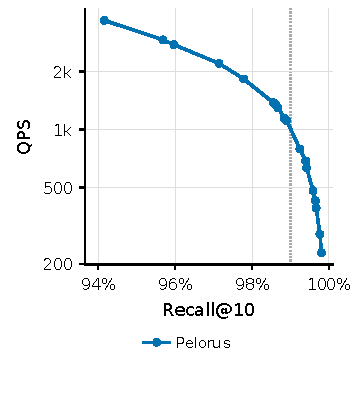
\includegraphics[width=0.8\linewidth]{pareto_openai_1536_1t.pdf}
  \caption{Measured \rquiver{} Recall@10--QPS frontier on {OpenAI-1536} ($990$K vectors, $1536$D, Zen~4, one query thread).}
  \label{fig:pareto_openai}
\end{figure}

\subsection{Comparison with Hyperbolic and Flat-Proxy Engines}
\label{subsec:eval_external}

\begin{table*}[t]
  \centering
  \caption{Measured comparison of \rquiver{} and baselines on {Cohere-1M} and {MERU-1M} (Zen~4, 32 build threads) at Recall@10 targets of $90\%$, $95\%$, $98\%$, $99\%$, and $99.5\%$. Panels (a) and (b) give main-sweep 1T and 24T QPS. The final block gives the independently tested log-map and quantized controls.}
  \label{tab:external_baselines}
  \footnotesize
  \setlength{\tabcolsep}{2pt}
  \begin{tabular}{@{}llrrrrrrrrr@{}}
\multicolumn{11}{@{}l}{\textbf{(a) Single-thread QPS}} \\
\toprule
\textbf{Dataset} & \textbf{Method} & \textbf{$M/L_c$} & \textbf{\shortstack{Build\\32T (s)}} & \textbf{\shortstack{Peak\\Rec@10}} & \textbf{$\ge90\%$} & \textbf{$\ge95\%$} & \textbf{$\ge98\%$} & \textbf{$\ge99\%$} & \textbf{$\ge99.5\%$} & \textbf{\shortstack{p99 (ms)\\at $99\%$}} \\
\midrule
Cohere-1M & Pelorus & 16/128 & 35.0 & 99.700\% & 4,939 & 4,939 & 2,907 & 1,930 & 738 & 0.62 \\
 & Faiss centered IP & 32/256 & 167.3 & 98.910\% & 1,652 & 830 & 127 & \missing & \missing & \missing \\
 & Faiss direction & 16/128 & 77.6 & 65.170\% & \missing & \missing & \missing & \missing & \missing & \missing \\
 & Faiss raw Lorentz-IP & 16/128 & 7.4 & 0.120\% & \missing & \missing & \missing & \missing & \missing & \missing \\
 & Milvus centered IP & 32/256 & 361.7 & 98.690\% & 252 & 238 & 76 & \missing & \missing & \missing \\
 & HDB FP32 dynamic & 32/256 & 414.8 & 96.780\% & 839 & 290 & \missing & \missing & \missing & \missing \\
 & HDB FP32 flat & 32/256 & 416.3 & 96.670\% & 946 & 279 & \missing & \missing & \missing & \missing \\
 & HDB FP64 dynamic & 32/256 & 866.5 & 94.430\% & 67 & \missing & \missing & \missing & \missing & \missing \\
 & HDB FP64 flat & 32/256 & 869.3 & 94.330\% & 74 & \missing & \missing & \missing & \missing & \missing \\
 & Exact-RobustPrune & 16/128 & 75.5 & 93.940\% & 629 & \missing & \missing & \missing & \missing & \missing \\
 & Polar-SQ8 & 16/128 & 66.9 & 99.780\% & 2,428 & 2,428 & 1,887 & 878 & 372 & 1.44 \\
 & Polar-FP32 & 16/128 & 190.2 & 99.783\% & 1,355 & 1,355 & 1,027 & 448 & 258 & 2.69 \\
\midrule
MERU-1M & Pelorus & 16/128 & 25.7 & 99.983\% & 5,846 & 4,521 & 2,547 & 2,547 & 1,669 & 0.50 \\
 & Faiss centered IP & 32/256 & 99.2 & 99.988\% & 4,312 & 2,800 & 1,903 & 1,059 & 872 & 1.43 \\
 & Faiss direction & 16/128 & 48.8 & 100.000\% & 3,460 & 1,814 & 1,480 & 1,078 & 1,078 & 1.30 \\
 & Faiss raw Lorentz-IP & 16/128 & 36.3 & 93.858\% & 841 & \missing & \missing & \missing & \missing & \missing \\
 & Milvus centered IP & 32/256 & 271.6 & 99.991\% & 297 & 297 & 297 & 260 & 233 & 5.30 \\
 & HDB FP32 dynamic & 16/128 & 86.5 & 99.947\% & 3,136 & 2,103 & 1,493 & 1,188 & 875 & 1.27 \\
 & HDB FP32 flat & 16/128 & 87.6 & 99.947\% & 3,187 & 2,184 & 1,579 & 1,296 & 966 & 1.15 \\
 & HDB FP64 dynamic & 32/256 & 631.4 & 99.955\% & 615 & 428 & 281 & 196 & 165 & 8.83 \\
 & HDB FP64 flat & 32/256 & 633.9 & 99.707\% & 480 & 320 & 186 & 93 & 46 & 21.68 \\
\bottomrule
\end{tabular}
\par\vspace{5pt}
\begin{tabular*}{\linewidth}{@{\extracolsep{\fill}}llrrrrr@{}}
\multicolumn{7}{@{}l}{\textbf{(b) 24-thread QPS (queries/s)}} \\
\toprule
\textbf{Dataset} & \textbf{Method} & \textbf{$\ge90\%$} & \textbf{$\ge95\%$} & \textbf{$\ge98\%$} & \textbf{$\ge99\%$} & \textbf{$\ge99.5\%$} \\
\midrule
Cohere-1M & Pelorus & 96,584 & 96,584 & 58,162 & 42,466 & 17,137 \\
 & Faiss centered IP & 10,717 & 10,717 & 1,660 & \missing & \missing \\
 & Faiss direction & \missing & \missing & \missing & \missing & \missing \\
 & Faiss raw Lorentz-IP & \missing & \missing & \missing & \missing & \missing \\
 & Milvus centered IP & 1,115 & 1,115 & 999 & \missing & \missing \\
 & HDB FP32 dynamic & 3,416 & 3,416 & \missing & \missing & \missing \\
 & HDB FP32 flat & 3,656 & 3,656 & \missing & \missing & \missing \\
 & HDB FP64 dynamic & \missing & \missing & \missing & \missing & \missing \\
 & HDB FP64 flat & \missing & \missing & \missing & \missing & \missing \\
 & Exact-RobustPrune & \missing & \missing & \missing & \missing & \missing \\
 & Polar-SQ8 & 46,034 & 46,034 & 34,639 & 16,844 & 7,016 \\
 & Polar-FP32 & 19,932 & 19,932 & 14,925 & 6,735 & 3,937 \\
\midrule
MERU-1M & Pelorus & 94,846 & 94,846 & 53,483 & 53,483 & 36,092 \\
 & Faiss centered IP & 33,189 & 33,189 & 22,488 & 13,005 & 9,349 \\
 & Faiss direction & 43,798 & 43,798 & 19,883 & 14,967 & 9,866 \\
 & Faiss raw Lorentz-IP & \missing & \missing & \missing & \missing & \missing \\
 & Milvus centered IP & 1,208 & 1,208 & 1,208 & 1,130 & 1,088 \\
 & HDB FP32 dynamic & 30,015 & 30,015 & 18,413 & 13,780 & 11,038 \\
 & HDB FP32 flat & 26,235 & 26,235 & 19,434 & 15,890 & 11,699 \\
 & HDB FP64 dynamic & 9,588 & 9,588 & 6,121 & 4,098 & 3,414 \\
 & HDB FP64 flat & 6,362 & 6,362 & 4,039 & 1,933 & 925 \\
\bottomrule
\end{tabular*}

  \par\smallskip
\begin{tabular*}{\linewidth}{@{\extracolsep{\fill}}lrrrrrr@{}}
\multicolumn{7}{@{}l}{\textbf{MERU-1M log-map and quantized controls ($99\%$ validation target, 10,000 test queries)}}\\
\toprule
& \multicolumn{3}{c}{1 thread} & \multicolumn{3}{c}{24 threads}\\
\cmidrule(lr){2-4}\cmidrule(l){5-7}
Method & Recall@10 (\%) & QPS & p99 (ms) & Recall@10 (\%) & QPS & p99 (ms)\\
\midrule
Faiss FP32 (log-map $L_2$) & 99.059 & 2,136 & 0.65 & 99.150 & 15,103 & 2.61\\
Faiss SQ8 (log-map $L_2$) & 99.119 & 1,220 & 1.07 & 99.119 & 26,786 & 1.28\\
Milvus SQ8 (centered IP) & 99.405 & 73 & 20.75 & 99.716 & 587 & 115.23\\
HDB SQ8 (Poincar\'e, FP64 rerank) & 99.224 & 763 & 1.85 & 99.224 & 13,620 & 2.52\\
Tangent 2-bit (paired engine) & 99.107 & 1,510 & 0.99 & 99.107 & 35,813 & 0.99\\
\rquiver{} 2-bit (paired engine) & 99.248 & 2,311 & 0.55 & 99.247 & 50,848 & 0.60\\
\bottomrule
\end{tabular*}

  \par\vspace{2pt}
  {\footnotesize \textit{Note:} HDB denotes HyperspaceDB. The paired-engine rows use a separate, sequentially timed comparison with validation-selected budgets. For \rquiver{}, $(L,B)$ is $(128,128)$ at 1T and $(128,32)$ at 24T. A dash denotes the absence of a qualifying measured point at that thread count. Build time and $M/L_c$ correspond to the fastest qualifying 1T configuration at $99\%$ recall, or the peak-recall configuration when $99\%$ is unreached. Each QPS column independently selects its fastest measured qualifying configuration. The $90\%$ and $95\%$ columns are selected from the existing measured configurations. Peak recall is the largest measured 1T recall; p99 is in milliseconds at the selected $99\%$ 1T point.}
\end{table*}

\begin{figure*}[t]
  \centering
  \begin{subfigure}[t]{0.485\textwidth}
    \centering
    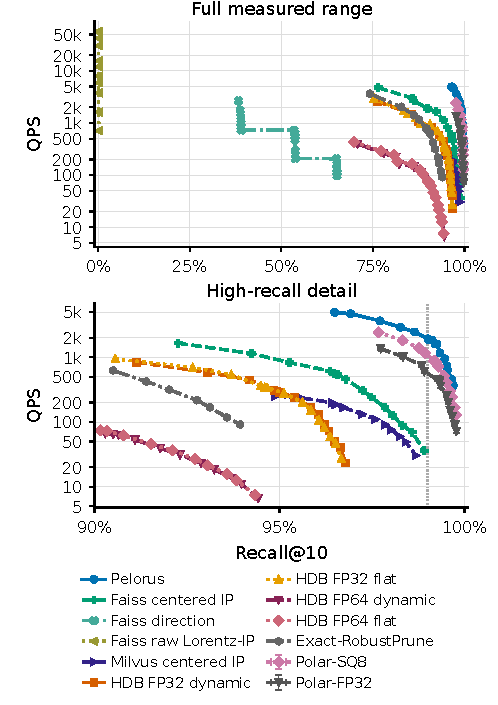
\includegraphics[width=\linewidth]{pareto_cohere_1m_1t.pdf}
    \caption{Cohere-1M ($768$D, 1 thread)}
    \label{fig:pareto_cohere}
  \end{subfigure}\hfill
  \begin{subfigure}[t]{0.485\textwidth}
    \centering
    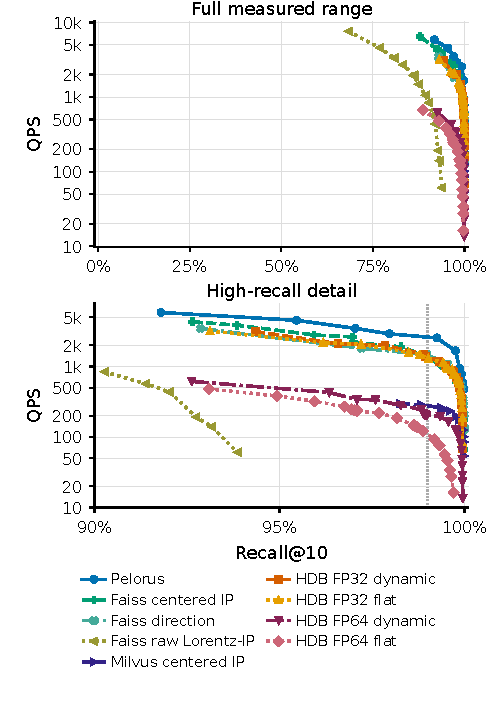
\includegraphics[width=\linewidth]{pareto_meru_1m_1t.pdf}
    \caption{MERU-1M ($512$D, 1 thread)}
    \label{fig:pareto_meru}
  \end{subfigure}
  \caption{Matched-dataset Recall@10--QPS frontiers of \rquiver{} and external baselines in the main Zen~4 sweep. Each panel shows the full measured recall range and a high-recall detail view. HDB denotes HyperspaceDB. Each method uses the first build per configuration (\S\ref{subsec:eval_setup}). Each method's frontier includes its measured build and search configurations; lines connect nondominated measurements.}
  \label{fig:real_pareto}
\end{figure*}

Table~\ref{tab:external_baselines} and Figure~\ref{fig:real_pareto} place \rquiver{} alongside {Exact-RobustPrune}~\cite{prokhorenkova2022hyperbolic}, {HDB} ({HyperspaceDB}~\cite{glukhota2026hyperspacedb}), and flat inner-product {HNSW} proxies in {Faiss}~\cite{douze2024faiss} ({Faiss centered IP}, {Faiss direction}, {Faiss raw Lorentz-IP}) and {Milvus}~\cite{wang2021milvus} ({Milvus centered IP}).
On the mapped {Cohere-1M} benchmark (Figure~\ref{fig:pareto_cohere}), \rquiver{} builds in $35.0$\,s, reaches $99.70\%$ peak Recall@10, and sustains $1{,}930$\,QPS (1T) and $42{,}466$\,QPS (24T) at $\ge 99\%$ recall.
On {Cohere-1M}, {Exact-RobustPrune} ($16/128$, $L\le2{,}048$) reaches $93.94\%$ peak Recall@10 ($75.5$\,s build), {HDB FP32 dynamic} and {HDB FP32 flat} ($32/256$) reach $96.78\%$ and $96.67\%$ ($414.8$\,s and $416.3$\,s build), and {HDB FP64 dynamic} and {HDB FP64 flat} ($32/256$) reach $94.43\%$ and $94.33\%$ ($866.5$\,s and $869.3$\,s); at the common $95\%$ recall target, \rquiver{} delivers $4{,}939$\,QPS (1T) and $96{,}584$\,QPS (24T) compared with $290$\,QPS (1T, $17.0\times$) and $3{,}416$\,QPS (24T, $28.3\times$) for {HDB FP32 dynamic}.
In the {Cohere-1M} flat {HNSW} sweeps ($ef\le4{,}096$), {Faiss centered IP} and {Milvus centered IP} ($32/256$) peak at $98.91\%$ and $98.69\%$ Recall@10 ($167.3$\,s and $361.7$\,s build; at $98\%$ recall, \rquiver{} attains $2{,}907$\,QPS on 1T and $58{,}162$\,QPS on 24T vs.\ $127$ / $1{,}660$\,QPS for {Faiss centered IP} and $76$ / $999$\,QPS for {Milvus centered IP}), while {Faiss direction} and {Faiss raw Lorentz-IP} reach $65.17\%$ and $0.12\%$. Under matched $M/L_c = 16/128$ ($ef \le 4{,}096$), external {Cohere-1M} peak recalls drop further to $93.84\%$/$93.64\%$ for {HDB FP32 dynamic/flat} ($106.1$\,s/$107.5$\,s build; $558$/$530$\,QPS 1T at $\ge 90\%$, missing $95\%$), $89.94\%$/$89.74\%$ for {HDB FP64}, and $97.93\%$/$97.99\%$ for {Faiss/Milvus centered IP} ($517$/$176$\,QPS 1T at $\ge 95\%$, missing $98\%$).

On {MERU-1M}, HDB FP32 flat reaches $1{,}296$/$15{,}890$\,QPS at $99.026\%$ recall and HDB FP32 dynamic reaches $1{,}188$/$13{,}780$ at $99.312\%$. At the $99\%$ target, \rquiver{} serves $1.97\times$/$3.37\times$ the HDB flat throughput (1T/24T).

\paragraph{SQ8 graph indices.}
On {MERU-1M}, HyperspaceDB SQ8 top-10 recall peaks at $63.93\%$ (Poincar\'e) and $51.75\%$ (Lorentz) across dynamic/flat layouts, $16/128$ and $32/256$ builds, and $ef\le4{,}096$. With the same cold FP32 vectors and $128$ candidates reranked in FP64, Poincar\'e SQ8 reaches $99.224\%$ at $763$/$13{,}620$\,QPS (1T/24T, $16/128$, $ef=256$). Lorentz SQ8 peaks at $96.66\%$ with this rerank budget.
Table~\ref{tab:official_sq8} evaluates Faiss \texttt{IndexHNSWSQ} on log-map $L_2$ and Milvus \texttt{HNSW\_SQ} on centered IP ($M/L_c=16/128$). At the $99\%$ validation target, Faiss serves $1{,}220/26{,}786$\,QPS at $99.119\%$ test recall (1T/24T). Milvus serves $73/587$\,QPS at $99.405/99.716\%$. Both systems test direct top-10 and FP64 geodesic reranking of 128 candidates. Faiss timings use the in-process C++ API. Milvus timings include the Python client and public gRPC call.

\begin{table}[!htbp]
 \centering
 \caption{MERU-1M with official SQ8 HNSW indices ($M/L_c=16/128$). For each target and thread count, $ef$ and $B$ are selected on 2,000 validation queries. Cells report outcomes on 10,000 test queries.}
 \label{tab:official_sq8}
 \footnotesize
 \setlength{\tabcolsep}{2.4pt}
 \begin{tabular}{@{}lrrrrrrr@{}}
 \toprule
 & Target & \multicolumn{3}{c}{One thread} & \multicolumn{3}{c}{24 threads}\\
 \cmidrule(lr){3-5}\cmidrule(lr){6-8}
 Engine & (\%) & R@10 (\%) & QPS & $p_{99}$ (ms) & R@10 (\%) & QPS & $p_{99}$ (ms)\\
 \midrule
Faiss & 98 & 98.463 & 1,961 & 0.74 & 98.463 & 41,457 & 0.88 \\
 & 99 & 99.119 & 1,220 & 1.07 & 99.119 & 26,786 & 1.28 \\
 & 99.5 & 99.578 & 973 & 1.37 & 99.578 & 20,805 & 1.65 \\
Milvus & 98 & 98.268 & 117 & 12.63 & 98.200 & 1,162 & 32.81 \\
 & 99 & 99.405 & 73 & 20.75 & 99.716 & 587 & 115.23 \\
 & 99.5 & 99.716 & 52 & 28.72 & 99.716 & 595 & 118.12 \\
 \bottomrule
 \end{tabular}
\end{table}


\paragraph{Tangent-space controls.}
Following {HyEm}'s candidate retrieval step~\cite{deng2026hyem}, we map $x$ to $\atanh(\|x\|)x/\|x\|$ (zero maps to zero). On {MERU-1M}, {Faiss} $L_2$ HNSW selects $M/L_c=16/128$ and $ef=128$ at both thread counts. Returning top-10 directly serves $2{,}136$\,QPS at $99.06\%$ recall on one thread. At 24 threads, FP64 geodesic reranking of 128 candidates serves $15{,}103$\,QPS at $99.15\%$. At the $99\%$ target, \rquiver{} serves $1.19\times$ and $3.54\times$ the FP32 log-map throughput at 1T and 24T, respectively. Each worker takes one query from a shared queue and searches single-threaded. On mapped {Cohere-1M}, log-map HNSW peaks at $86.42\%$ on its separate 500-query test subset.

We also compare the two navigation metrics inside the same Rust engine on {MERU-1M} (Table~\ref{tab:tangent_sm}). The tangent graph stores the log-map norm $t_v=\atanh(\|v\|)$ and the same 2-bit {SM} direction as \rquiver{}. It uses $(t_q-t_v)^2+2t_qt_v(1-\hat\gamma_{qv})$ for squared Euclidean distance in construction and beam search. Ordinary isotropic RobustPrune uses $\alpha=1.2$, fills unused slots by distance, and inserts vertices in input order. Search starts from one entry. Both graphs use $M_0=32$, $L_c=128$, the original FP32 vectors, and the same FP64 geodesic reranker.

We ran the two methods serially. Rayon distributed independent queries across workers. We warmed each condition with 200 queries. For each method and thread count, the first build selected the fastest $(L,B)$ reaching $99\%$ recall on 2,000 validation queries. We then measured the frozen settings on 10,000 disjoint test queries using the first build.

\begin{table*}[t]
  \centering
  \caption{MERU-1M tangent-space and native 2-bit graphs on the independent test queries. Each method uses its first build.}
  \label{tab:tangent_sm}
  \small
  \begin{tabular*}{\linewidth}{@{\extracolsep{\fill}}lrrrrrrrrrr@{}}
    \toprule
    & \multicolumn{5}{c}{1 thread} & \multicolumn{5}{c}{24 threads} \\
    \cmidrule(lr){2-6}\cmidrule(l){7-11}
    Method & $(L,B)$ & Recall@10 & QPS & p99 (ms) & RSS (MiB) & $(L,B)$ & Recall@10 & QPS & p99 (ms) & RSS (MiB) \\
    \midrule
    \multicolumn{11}{@{}l}{\emph{Fixed candidate and rerank budgets}} \\
  Tangent 2-bit & $(128,128)$ & 97.837\% & 2,326 & 0.644 & 2,605 & $(128,128)$ & 97.837\% & 55,121 & 0.660 & 2,609 \\
  \rquiver{} & $(128,128)$ & 99.248\% & 2,248 & 0.555 & 2,722 & $(128,128)$ & 99.248\% & 51,733 & 0.592 & 2,726 \\
    \midrule
    \multicolumn{11}{@{}l}{\emph{Validation-selected operating points}} \\
  Tangent 2-bit & $(256,128)$ & 99.107\% & 1,510 & 0.989 & 2,609 & $(256,128)$ & 99.107\% & 35,813 & 0.993 & 2,605 \\
  \rquiver{} & $(128,128)$ & 99.248\% & 2,311 & 0.548 & 2,725 & $(128,32)$ & 99.247\% & 50,848 & 0.599 & 2,722 \\
    \bottomrule
  \end{tabular*}
  \par
  {\footnotesize $B$ is the nominal rerank budget. When $B<L$, \textsc{CJ-Gate} can admit additional candidates in \rquiver{}. Rows are timed independently. RSS includes cold vectors.}
\end{table*}


With $L=B=128$, all candidates reach reranking. Single-thread throughput is similar, and Recall@10 is 1.411 percentage points higher for \rquiver{}. At the validation-selected $99\%$ target, the tangent graph doubles its beam width to 256. \rquiver{} sustains $1.53\times$ its throughput at 1T and $1.42\times$ at 24T, using $516.8$ versus $428.0$\,MB of hot navigation memory. Both graphs have 32 million edges per build. All million vertices are reachable from \rquiver{}'s entries, compared with $999{,}701$ from the tangent graph's entry.

\subsection{Multi-Threaded Scaling Efficiency}
\label{subsec:eval_scaling}

\begin{figure*}[t]
  \centering
  \begin{subfigure}[t]{0.485\linewidth}
    \centering
    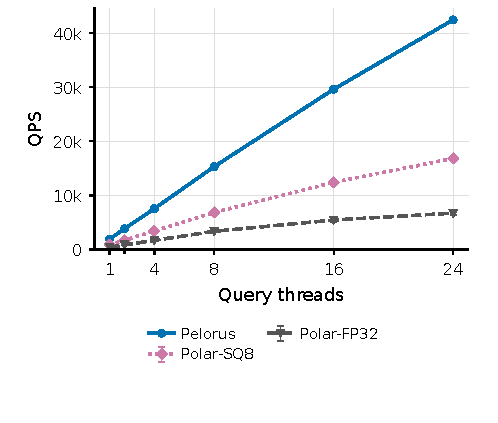
\includegraphics[width=\linewidth]{scaling_cohere_1m_r99.pdf}
    \caption{Cohere-1M ($\ge 99\%$ Recall)}
    \label{fig:scale_cohere}
  \end{subfigure}\hfill
  \begin{subfigure}[t]{0.485\linewidth}
    \centering
    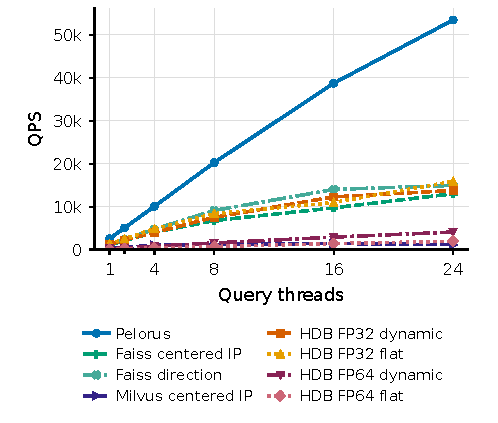
\includegraphics[width=\linewidth]{scaling_meru_1m_r99.pdf}
    \caption{MERU-1M ($\ge 99\%$ Recall)}
    \label{fig:scale_meru}
  \end{subfigure}
  \caption{Multi-threaded query scaling from 1 to 24 threads on Zen~4 at Recall@10 $\ge 99\%$. On {Cohere-1M}, \rquiver{} is compared against {Polar-SQ8} and {Polar-FP32} (external baseline peak recalls are reported in Table~\ref{tab:external_baselines}). On {MERU-1M}, \rquiver{} is compared against the main-sweep systems reaching $99\%$ recall. Each method selects its fastest qualifying configuration per thread count.}
  \label{fig:scaling}
\end{figure*}

Figure~\ref{fig:scaling} reports throughput scaling on the original sweep graph from $1$ to $24$ threads at $\ge 99\%$ Recall@10.
On {Cohere-1M} ($D=768$), the split-array and page layouts allocate $485.0$ and $517.0$\,MB of active navigation arrays, respectively (Table~\ref{tab:memory_audit}). Each page-layout slot holds a $64$\,B header including the sketch and $192$\,B of bitplanes. With read-only traversal, \rquiver{} scales by \textbf{$22.0\times$} at 24 threads on {Cohere-1M} ($1{,}930 \to 42{,}466$\,QPS, $91.7\%$ parallel efficiency; Figure~\ref{fig:scale_cohere}), \textbf{$21.0\times$} on {MERU-1M} ($2{,}547 \to 53{,}483$\,QPS), \textbf{$18.6\times$} on {OpenAI-1536} ($792 \to 14{,}731$\,QPS), and \textbf{$21.2\times$} on {WordNet-Hazy} ($3{,}089 \to 65{,}405$\,QPS).
By contrast, {Polar-FP32} reads $3{,}072$\,B ($48$ cache lines) per visited neighbor across a $3.37$\,GB footprint and scales by $15.3\times$ at 24 threads on {Cohere-1M} ($457 \to 7{,}004$\,QPS), widening \rquiver{}'s speedup from $4.23\times$ (1T) to \textbf{$6.06\times$ (24T)}; similarly, on {MERU-1M} (Figure~\ref{fig:scale_meru}), in-process FP32 systems scale by $11.6\times\text{--}12.3\times$ ({HDB FP32 dynamic/flat}: $1{,}188 \to 13{,}780$\,QPS and $1{,}296 \to 15{,}890$\,QPS; {Faiss centered IP}: $1{,}059 \to 13{,}005$\,QPS) and {Milvus centered IP} scales by $4.3\times$ ($260 \to 1{,}130$\,QPS), further widening \rquiver{}'s multi-threaded lead.

\subsection{Page Layout and Cold Storage}
\label{subsec:eval_storage}

With topology, code and query order fixed on the first {MERU-1M} builds, compact pages hold 21 vertices per page at $D=512$, up from 16. The allocated pages occupy $186.0$ versus $244.1$\,MiB. At $(L,B)=(128,64)$ both layouts return identical IDs and scores ($99.249\%$ recall). Single-thread throughput falls from $2{,}416$ to $2{,}305$\,QPS, while 24T rises from $47{,}470$ to $51{,}088$. On $65{,}536$-point probes derived from MERU, page allocations fall from $16.00$ to $10.24$\,MiB at $D=384$ and from $32.00$ to $21.34$\,MiB at $D=1024$. On $768$D {Cohere-1M}, both layouts occupy $244.1$\,MiB. At the same budget, compact pages serve $41{,}336$ versus $53{,}323$\,QPS at 24T. On $20$D {WordNet-Hazy}, compact pages use $6.43$ versus $10.25$\,MiB. Traversal can also share the cold FP32 vectors, eliminating separate code pages. Relative to the default pages, 1T process RSS falls from $70.5$ to $63.9$\,MiB. Recall rises from $97.340\%$ to $99.980\%$ while throughput falls from $4{,}578$ to $4{,}076$\,QPS.

The two layouts agree on returned IDs and scores at both measured budgets on every dimension. At $(256,128)$ on the first {Cohere-1M} build, compact and default pages reach $30{,}123/32{,}965$\,QPS at 24T with identical $99.260\%$ recall (Table~\ref{tab:layout_sweep}). Both layouts share a page translation per record. Packing also changes cache-line placement and address calculation. The container denied access to dTLB and LLC miss counters, so these timings measure the combined layout effect. Appendix~\ref{app:storage_measurements} reports both budgets, including process RSS and p99.

\begin{table}[t]
  \centering
  \caption{Cold reranking on {MERU-1M}. The 2-bit navigation graph stays in RAM. All rows use 24 threads, a 512\,MiB SSD cache and $\Delta_0=0.20$. The last column gives SSD bytes read per timed query in KiB.}
  \label{tab:meru_ssd}
  \footnotesize
  \setlength{\tabcolsep}{3pt}
  \begin{tabular}{@{}llrrrr@{}}
    \toprule
    Cold encoding & $L/B$ & Recall@10 & QPS & p99 (ms) & KiB/q \\
    \midrule
    FP32           & 512/128 & 99.917\% & 1,886 & 48.78 & 670.85 \\
    Cartesian FP16  & 512/128 & 99.902\% & 3,282 & 17.26 & 358.32 \\
    Polar FP16     & 512/128 & 99.902\% & 3,270 & 16.83 & 361.73 \\
    \midrule
    Centered SQ8    & 64/64 & 97.519\% & 23,760 & 4.48 & 44.31 \\
    Centered SQ4    & 64/64 & 90.123\% & 33,823 & 4.09 & 21.24 \\
    \bottomrule
  \end{tabular}
\end{table}

For SSD reranking we fix one graph, tune on $2{,}000$ queries, then time each condition once on $10{,}000$ test queries after 200 warmups. Batched \texttt{io\_uring} reads have a 32\,MiB in-flight budget. Polar FP16 and centered SQ4 retain an FP64 radius. At $L=512$, both FP16 formats nearly halve SSD traffic while retaining $99.902\%$ recall (Table~\ref{tab:meru_ssd}). At $L=64$, SQ4 reads $52\%$ fewer bytes per query than SQ8 and serves $42\%$ more queries per second at a cost of $7.396$ recall points. The highest SQ4 recall among the 43 configurations retested is $91.240\%$.

With cold FP32 and $99.917\%$ recall at 24T, moving from RAM to a 128\,MiB SSD cache cuts process RSS from $2.573$ to $0.825$\,GiB and throughput from $22{,}822$ to $1{,}308$\,QPS. At $(L,B)=(164,64)$, centered SQ8 returns the same top-10 results ($99.003\%$ recall) in RAM and with either cache. At 24T, RAM serves $51{,}040$\,QPS at $0.62$\,ms p99 and $1.155$\,GiB process RSS. Increasing the SSD cache from 128 to 512\,MiB cuts reads per query from $103.35$ to $10.00$, raises throughput from $2{,}749$ to $20{,}136$\,QPS, and lowers p99 from $23.87$ to $7.23$\,ms. RSS rises from $0.839$ to $1.228$\,GiB. Appendix~\ref{app:storage_measurements} lists 1T and 24T results for all five encodings with both cache budgets and RAM.
\subsection{Geometry and Execution Ablation Study}
\label{subsec:eval_ablation}

\begin{table}[t]
  \centering
  \caption{Controlled component ablations around {\rquiver{}-Core} on {Cohere-1M} (one thread, first build).}
  \label{tab:ablation_cohere}
  \small
  \setlength{\tabcolsep}{3pt}
  \begin{tabular}{@{}lrrrr@{}}
    \toprule
    & \textbf{Zero-In} & \textbf{Build} & \multicolumn{2}{c}{\textbf{1T QPS (p99 ms)}} \\
    \cmidrule(lr){4-5}
    \textbf{Variant} & \textbf{Islands} & \textbf{32T (s)} & \textbf{$\ge 99\%$} & \textbf{$\ge 99.5\%$} \\
    \midrule
    \textbf{\rquiver{}-Core} & 0 & 32.8 & 2,003 (0.59) & 687 (1.64) \\
    w/o \texttt{SymSketch256} & 0 & 32.8 & 1,850 (0.61) & 593 (1.97) \\
    w/o \texttt{HotSmPage} (SoA) & 0 & 32.8 & 1,701 (0.65) & 535 (2.14) \\
    SoA, \textsc{Stage-0.5} off & 0 & 32.8 & 1,665 (0.72) & 391 (2.83) \\
    SoA, Chord-Swap off & 521 & 32.4 & 1,739 (0.67) & 544 (2.06) \\
    \bottomrule
  \end{tabular}
\end{table}

\begin{figure*}[t]
  \centering
  \begin{subfigure}[t]{0.435\linewidth}
    \centering
    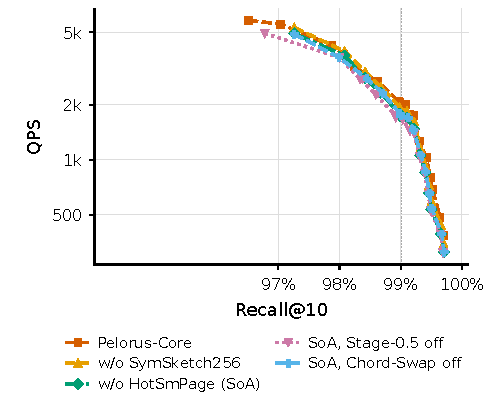
\includegraphics[width=\linewidth]{ablation_geometry_cohere_1m.pdf}
    \caption{Cohere-1M, topology and search}
    \label{fig:abl_geom}
  \end{subfigure}\hfill
  \begin{subfigure}[t]{0.435\linewidth}
    \centering
    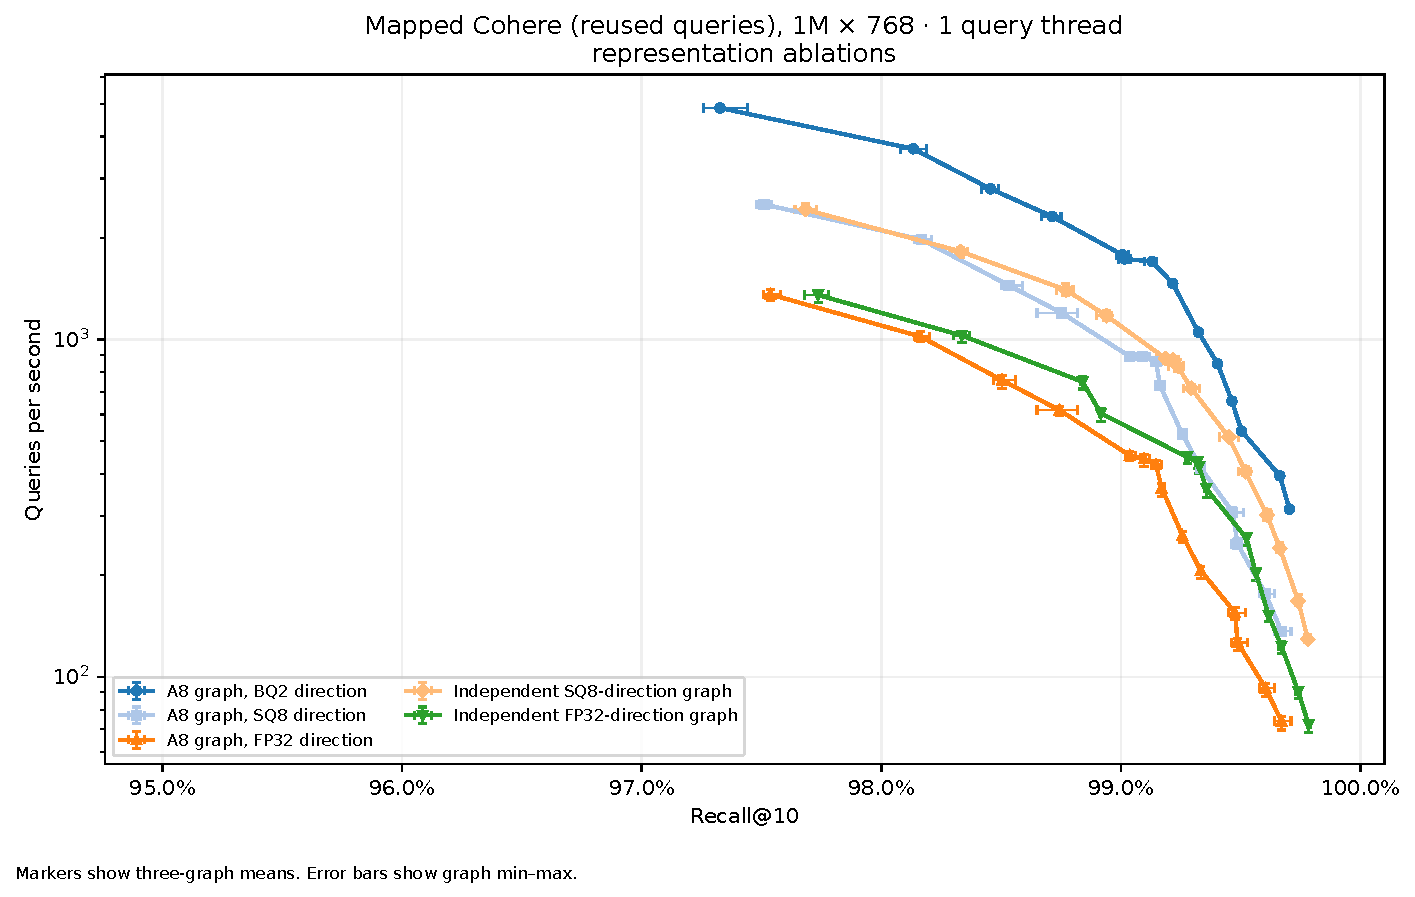
\includegraphics[width=\linewidth]{ablation_representation_cohere_1m.pdf}
    \caption{Cohere-1M, search representation}
    \label{fig:abl_repr}
  \end{subfigure}
  \par\smallskip
  \begin{subfigure}[t]{0.89\linewidth}
    \centering
    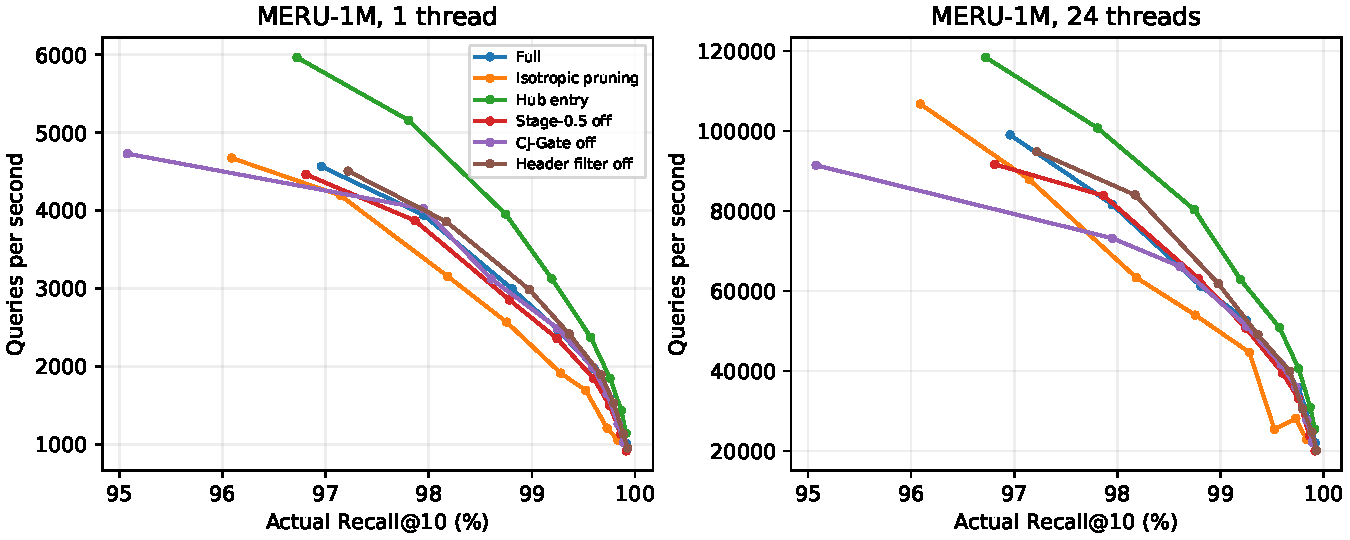
\includegraphics[width=\linewidth]{meru_ablation.pdf}
    \caption{MERU-1M, topology and search at eight fixed budgets.}
    \label{fig:abl_native}
  \end{subfigure}
  \caption{Component ablations on the first build. The upper panels give single-thread frontiers on {Cohere-1M}. The lower panels give measured recall and throughput at eight fixed budgets on {MERU-1M}.}
  \label{fig:ablation_pdf}
\end{figure*}
\begin{table}[t]
 \centering
 \caption{Pruning policies on Cohere-1M with the Core query engine. Fixed-budget Recall@10 uses $(L,B)=(192,64)$. Peak recall and the fastest 1T point reaching $99\%$ use the same 16 budgets for each policy ($L\le 2{,}048$). The final two rows are the first pair from an independent three-seed rebuild.}
 \label{tab:cohere_channels}
 \footnotesize
 \setlength{\tabcolsep}{3pt}
 \begin{tabular}{@{}lrrrrr@{}}
 \toprule
 & \multicolumn{2}{c}{Recall (\%)} & \multicolumn{3}{c}{$\ge 99\%$ Recall@10} \\
 \cmidrule(lr){2-3}\cmidrule(lr){4-6}
 Policy & Fixed & Peak & $L/B$ & QPS & p99 (ms)\\
 \midrule
All four channels & 99.00 & 99.70 & 192/64 & 1,957 & 0.58 \\
Geodesic off & 99.41 & 99.91 & 192/64 & 1,874 & 0.63 \\
Ring off & 97.09 & 98.74 & \missing & \missing & \missing \\
Inward elevator off & 99.08 & 99.73 & 192/64 & 1,928 & 0.61 \\
Outward elevator off & 99.00 & 99.65 & 208/64 & 1,972 & 0.58 \\
Both elevators off & 99.23 & 99.71 & 192/64 & 1,925 & 0.59 \\
Ring shield off & 98.99 & 99.69 & 200/64 & 1,896 & 0.62 \\
Earlier two-pass & 97.55 & 99.44 & 1536/64 & 426 & 2.64 \\
 \midrule
QuadriPrune (paired) & 98.97 & 99.72 & 200/64 & 1,946 & 0.60 \\
Angular quota (paired) & 98.93 & 99.87 & 208/64 & 1,721 & 0.68 \\
 \bottomrule
 \end{tabular}
\end{table}

\paragraph{Cohere-1M.}
The left and right Cohere panels in Figure~\ref{fig:ablation_pdf} use the first build in Table~\ref{tab:ablation_cohere}. The first varies topology and query decisions. The second holds the search policy in split-array form and changes the directional representation.
\begin{itemize}
  \item \emph{QuadriPrune.}
  The earlier two-pass policy first allocates up to $5M_0/8$ slots using directional-signature screening and a depth-adjusted geodesic dominance test. It fills the rest in order of signature distance plus a shell penalty, pruning within nearby shells before backfilling. For the observed {Cohere-1M} depth range $[0.98,3.39]$, the all-angle sufficient bound in Theorem~\ref{thm:vamana_pathologies}(1) extends at most to $(3.39-1.2\cdot0.98)/2.2\approx1.01$, below the first percentile of $1.45$. Beyond this sufficient bound, the theorem alone does not determine which candidates are occluded. Table~\ref{tab:cohere_channels} rebuilds each policy with the same seed and runs the same co-located Core engine, sketch, and reranker. QuadriPrune reaches $99\%$ at $L=192$, versus $1{,}536$ for the two-pass policy ($1{,}957$ versus $426$\,QPS). Removing the ring drops fixed-budget recall by $1.91$ points. Keeping the ring and allowing cross-shell occlusion changes recall by just $0.01$ points. Removing both elevators gives $99.23\%$ at the fixed budget and preserves full reachability on all three seeds. Removing either elevator also preserves the target, while removing the geodesic channel raises fixed-budget recall to $99.41\%$. Of the individual channel removals, only ring removal misses $99\%$ on all three seeds (peak $98.74$--$98.80\%$).

We also rebuilt QuadriPrune alongside a simpler graph for each of three seeds, alternating the run order. The simpler policy ranks candidates by two-bit angular loss and selects up to 16 of 32 neighbors by angular diversity ($\alpha=1.2$), with neither a shell shield nor dedicated geodesic or elevator passes. Both policies then use the same depth-aware refill, chord repair, entries and Core scoring. All six graphs reach every vertex with 32 million directed edges. In the first pair at the $99\%$ target, QuadriPrune serves $1{,}946$\,QPS at $99.08\%$ recall and the quota graph $1{,}721$ at $99.03\%$. At the $99.5\%$ target, the quota graph needs $L=384$ on all three builds ($1{,}057$--$1{,}064$\,QPS), while QuadriPrune needs $L=768$--$1{,}024$ ($638$--$786$\,QPS), all at $B=128$. Thus the throughput advantage on this shell changes direction with the recall target.
  \item \emph{\textsc{Stage-0.5} asymmetric refinement.}
  On the split-array path, ordering the pool by the calibrated hop score alone reduces $99.5\%$ throughput from $535$ to $391$\,QPS. At $99\%$ the two paths serve $1{,}701$ and $1{,}665$\,QPS.
  \item \emph{Spanning-Tree Chord-Swap Repair:}
  On the unrepaired build in this ablation, 521 vertices have zero in-degree and 530 are unreachable from the entry hub. Split-array throughput at $99\%$ is $1{,}739$\,QPS without repair and $1{,}701$ with it.
  \item \emph{\texttt{HotSmPage} and \texttt{SymSketch256}.}
  At $99\%$ recall, page co-location raises 1T throughput from $1{,}701$ to $1{,}850$\,QPS. Adding the sketch raises it to $2{,}003$\,QPS. At $99.5\%$ these configurations serve $535$, $593$ and $687$\,QPS.
\end{itemize}

A $2\times2$ query-side ablation holds the full Cohere graph, PolarRouter and six budgets fixed. Switching \textsc{CJ-Gate} preserves the IDs and scores for all $1{,}000$ queries at every budget. With the gate off, sketch-margin calibration at $(L,B,\Delta_0)=(192,64,0.12)$ moves recall from $99.00$ to $99.03\%$ and 1T throughput from $1{,}960$ to $1{,}800$\,QPS. At $(64,64,0.20)$ it moves recall from $98.15$ to $97.94\%$. At $(768,128,0.12)$ it moves recall from $99.49$ to $99.52\%$, making this smaller beam eligible at the highest target.

A separate entry comparison on one Cohere Core graph selects $L=512$ for PolarRouter and $768$ for hubs alone at a $99.5\%$ tuning target ($B=128$ for both). On the 500 held-out queries, PolarRouter reaches $99.30\%$ recall at $977/20{,}055$\,QPS (1T/24T), and hubs alone reach $99.20\%$ at $818/16{,}657$\,QPS. A separate header trace inspects 32 queries per seed. On Cohere the radial bound by itself rejects zero candidates. The default sketch test rejects $51.65\%$ of inspected candidates, falling to $45.82\%$ when the radial term is removed from that test.

\paragraph{MERU-1M.}
Figure~\ref{fig:abl_native} uses one graph for all query switches. The isotropic control rebuilds the graph with the same degree, refill and repair. It discards candidate $v$ at $u$ if a selected $p$ satisfies $\alpha\tilde d(p,v)\le\tilde d(u,v)$, where $\tilde d$ is the geodesic distance estimate recovered from the quantized proxy. At $L=B=128$, QuadriPrune raises recall from $98.755\%$ to $99.251\%$ ($2{,}568$ to $2{,}470$\,QPS, 1T). At $(256,128)$, hub-only entry serves $1{,}848$ versus $1{,}588$\,QPS for the full router ($99.757/99.754\%$ recall). Removing \textsc{Stage-0.5} or the header filter gives $33{,}206$ or $30{,}593$\,QPS at 24T versus $35{,}872$ for the full method. Disabling \textsc{CJ-Gate} gives $36{,}031$\,QPS and $99.729\%$ recall.

The eight search budgets are fixed before measuring the 10,000 native test queries. At $(256,128)$ the full method and hub-only entry serve $35{,}872$ and $40{,}594$\,QPS at 24T. In the MERU header trace the radial bound alone again rejects zero. The default and radial-term-removed sketch tests reject $50.03\%$ and $49.98\%$.

Table~\ref{tab:auto_entry} uses validation queries to choose between hubs and PolarRouter together with $(L,B)$ on a full graph, independently at each target and thread count. At each of the 14 budgets both entries use the same graph and reranker. MERU uses its usual validation and test sets, and Cohere uses the archived 500/500 split. MERU selects hubs at all six operating points. At the $99\%$ target, fixed PolarRouter reaches $99.250\%$ at $2{,}272/49{,}731$\,QPS, while automatic entry reaches $99.203/99.202\%$ at $2{,}868/64{,}786$\,QPS. Each automatic run returns exactly the IDs and scores of its selected fixed policy. Timing either policy once can change the throughput ordering: at the $99.5\%$ MERU target and 24T, automatic entry serves $38{,}842$\,QPS versus $40{,}175$ for fixed PolarRouter. The 16 hubs bypass both cone scans on shallow MERU. At the $99.5\%$ validation target on Cohere, 1T selects PolarRouter with $L=512$ (hubs require $768$), while 24T selects hubs. Held-out recall is $99.36\%$ and $99.22\%$, respectively.

\begin{table}[t]
\centering
\caption{Automatic entry selection for full \rquiver{}. On each validation set we choose the fastest qualifying combination of entry, $L$ and $B$ at each thread count. Recall and QPS are measured on held-out queries. H denotes hubs alone and P denotes PolarRouter.}
\label{tab:auto_entry}
\footnotesize
\setlength{\tabcolsep}{2.5pt}
\begin{tabular}{@{}lrrrrrrr@{}}
\toprule
& Target & \multicolumn{3}{c}{One thread} & \multicolumn{3}{c}{24 threads}\\
\cmidrule(lr){3-5}\cmidrule(lr){6-8}
Dataset & (\%) & Entry & R@10 (\%) & QPS & Entry & R@10 (\%) & QPS\\
\midrule
MERU-1M & 98 & H & 98.745 & 3,801 & H & 98.745 & 80,145 \\
 & 99 & H & 99.203 & 2,868 & H & 99.202 & 64,786 \\
 & 99.5 & H & 99.580 & 2,270 & H & 99.640 & 38,842 \\
Cohere-1M & 98 & H & 98.260 & 3,237 & H & 98.260 & 46,870 \\
 & 99 & H & 99.060 & 1,875 & H & 99.060 & 36,580 \\
 & 99.5 & P & 99.360 & 921 & H & 99.220 & 17,031 \\
\bottomrule
\end{tabular}
\end{table}


\paragraph{Pruning channels.}
Table~\ref{tab:pruning_controls} holds degree, refill and repair fixed. At $L=B=128$ on MERU and $(256,128)$ on HyperE WordNet, removing the geodesic channel changes recall by $+0.03$ and $-9.02$ points on the first build. On WordNet the other channel removals change recall by at most $0.32$ points. Ring width and elevator gap move recall by at most $0.43$ points across the tested settings. In the quota sweep all vertices remain reachable at 32 outgoing edges per vertex. The largest fixed-budget losses come from removing the ring on hollow-shell Cohere and geodesic edges on deep WordNet. Elevators supply cross-shell links within the fixed degree budget. On Cohere, removing both preserves the $99\%$ target.

\begin{table}[t]
  \centering
  \caption{QuadriPrune controls on shallow MERU and deep HyperE WordNet. Cells give Recall@10 (\%) on the first build. Each block has its own default.}
  \label{tab:pruning_controls}
  \footnotesize
  \setlength{\tabcolsep}{4pt}
  \begin{tabular}{@{}lrr@{}}
    \toprule
    Construction setting & MERU-1M & HyperE WordNet \\
    \midrule
  Default & 99.254 & 68.516 \\
  Geodesic off & 99.288 & 59.492 \\
  Ring off & 99.254 & 68.203 \\
  Inward elevator off & 99.255 & 68.555 \\
  Outward elevator off & 99.258 & 68.555 \\
  Ring width 0.30 & 99.254 & 68.945 \\
  Ring width 0.90 & 99.253 & 68.555 \\
  Elevator gap 0.09 & 99.252 & 68.672 \\
  Elevator gap 0.27 & 99.255 & 68.828 \\
    \midrule
    \multicolumn{3}{@{}l}{Geodesic and cumulative ring quotas (sixteenths)}\\
  6, 14 (default) & 99.251 & 68.555 \\
  4, 14 & 99.289 & 67.969 \\
  8, 14 & 99.207 & 68.945 \\
  6, 12 & 99.253 & 68.477 \\
  6, 15 & 99.255 & 68.711 \\
    \bottomrule
  \end{tabular}
\end{table}


\subsection{Synthetic Stress Tests, Recall-Loss Audit, and Applicability Boundaries}
\label{subsec:eval_synthetic}

\begin{table}[t]
  \centering
  \caption{Single-build sweep on synthetic extreme manifolds and real-manifold trade-offs on Zen~4 (complete \rquiver{} with tangent-cone rescue and adaptive \textsc{CJ-Gate} vs.\ \textbf{Global-SM} without cone rescue or \textsc{CJ-Gate}, $0$\,B/vertex overhead).}
  \label{tab:synthetic_rescue}
  \footnotesize
  \setlength{\tabcolsep}{1.7pt}
  \begin{tabular}{@{}lrrrrrr@{}}
    \toprule
    & \multicolumn{2}{c}{\textbf{Peak (\%)}} & & \multicolumn{3}{c}{\textbf{QPS at row target}} \\
    \cmidrule(lr){2-3}\cmidrule(lr){5-7}
    \textbf{Dataset (target)} & \textbf{\shortstack{Global\\SM}} & \textbf{\rquiver{}} & \textbf{Cones} & \textbf{\shortstack{Global\\SM 1T}} & \textbf{Full 1T} & \textbf{Full 24T} \\
    \midrule
    Clustered-Narrow & 34.220 & \textbf{99.945} & 256 & \emph{Unr.} & \textbf{1,840} & \textbf{38,876} \\
    Clustered-Wide & 73.865 & \textbf{99.995} & 256 & \emph{Unr.} & \textbf{2,704} & \textbf{57,144} \\
    Uniform-Wide ($98\%$) & 97.930 & \textbf{98.880} & 0 & \emph{Unr.} & $^\dagger$\emph{300} & $^\dagger$\emph{6,739} \\
    Uniform-Narrow & 62.410 & \textbf{64.735}$^\ddagger$ & 0 & \emph{Unr.} & \emph{Unr.} & \emph{Unr.} \\
    \midrule
    Cohere-1M ($99\%$) & 99.700 & \textbf{99.700} & 0 & \textbf{1,932} & 1,930 & 42,466 \\
    Cohere-1M ($99.5\%$) & 99.700 & \textbf{99.700} & 0 & 451 & \textbf{738} & \textbf{17,137} \\
    MERU-1M ($99\%$) & 99.952 & \textbf{99.983} & 0 & 1,443 & \textbf{2,547} & \textbf{53,483} \\
    MERU-1M ($99.5\%$) & 99.952 & \textbf{99.983} & 0 & 1,443 & \textbf{1,669} & \textbf{36,092} \\
    OpenAI-1536 ($99\%$) & 99.808 & \textbf{99.809} & 0 & \textbf{820} & 792 & 14,731 \\
    OpenAI-1536 ($99.5\%$) & 99.808 & \textbf{99.809} & 0 & \textbf{487} & 481 & 9,094 \\
    \bottomrule
  \end{tabular}
  \par\vspace{2pt}
  {\footnotesize\raggedright Peaks give 1T Recall@10. Unmarked rows have a $99\%$ throughput target. $^\dagger$At $\ge 98\%$ Recall@10 ($98.51\%$ at $L=1{,}536, B=128$; {Global-SM} caps at $97.93\%$). $^\ddagger$On the 32-query diagnostic probe, FP64 geodesic traversal on the same degree-32 graph visits and returns 199 of 320 true neighbors ($62.2\%$, $\mathcal{L}_{\mathrm{reach}}=37.8\%,\ \mathcal{L}_{\mathrm{beam}}=\mathcal{L}_{\mathrm{gate}}=0\%$), characterizing traversal loss on this constructed graph.\par}
\end{table}

\begin{table*}[t]
  \centering
  \caption{Measured comparison on all four synthetic distributions (1M vectors, 512D, Zen~4). Each QPS column selects the fastest measured configuration reaching its Recall@10 threshold. Panels (a) and (b) report one and 24 query threads.}
  \label{tab:synthetic_external}
  \footnotesize
  \setlength{\tabcolsep}{2pt}
  \begin{tabular}{@{}llrrrrrrrrr@{}}
\multicolumn{11}{@{}l}{\textbf{(a) Single-thread QPS}} \\
\toprule
\textbf{Dataset} & \textbf{Method} & \textbf{$M/L_c$} & \textbf{\shortstack{Build\\32T (s)}} & \textbf{\shortstack{Peak\\Rec@10}} & \textbf{$\ge90\%$} & \textbf{$\ge95\%$} & \textbf{$\ge98\%$} & \textbf{$\ge99\%$} & \textbf{$\ge99.5\%$} & \textbf{\shortstack{p99 (ms)\\at $99\%$}} \\
\midrule
Uniform-Narrow & Pelorus & 16/128 & 46.8 & 64.735\% & \missing & \missing & \missing & \missing & \missing & \missing \\
 & HDB FP32 flat & 32/256 & 478.2 & 92.170\% & 18 & \missing & \missing & \missing & \missing & \missing \\
 & Faiss centered IP & 32/256 & 311.3 & 29.860\% & \missing & \missing & \missing & \missing & \missing & \missing \\
 & Milvus centered IP & 32/256 & 573.6 & 46.445\% & \missing & \missing & \missing & \missing & \missing & \missing \\
\midrule
Uniform-Wide & Pelorus & 16/128 & 31.9 & 98.880\% & 639 & 397 & 300 & \missing & \missing & \missing \\
 & HDB FP32 flat & 32/256 & 299.6 & 97.860\% & 241 & 103 & \missing & \missing & \missing & \missing \\
 & Faiss centered IP & 32/256 & 140.1 & 48.640\% & \missing & \missing & \missing & \missing & \missing & \missing \\
 & Milvus centered IP & 32/256 & 255.1 & 54.040\% & \missing & \missing & \missing & \missing & \missing & \missing \\
\midrule
Clustered-Narrow & Pelorus & 16/128 & 25.3 & 99.945\% & 3,371 & 2,875 & 2,092 & 1,840 & 1,551 & 0.67 \\
 & HDB FP32 flat & 32/256 & 106.4 & 99.950\% & 1,568 & 1,315 & 1,133 & 998 & 998 & 1.33 \\
 & Faiss centered IP & 32/256 & 35.2 & 21.245\% & \missing & \missing & \missing & \missing & \missing & \missing \\
 & Milvus centered IP & 32/256 & 146.8 & 19.525\% & \missing & \missing & \missing & \missing & \missing & \missing \\
\midrule
Clustered-Wide & Pelorus & 16/128 & 19.4 & 99.995\% & 4,113 & 3,572 & 3,141 & 2,704 & 2,704 & 0.44 \\
 & HDB FP32 flat & 32/256 & 73.7 & 99.500\% & 1,037 & 908 & 735 & 735 & 645 & 2.14 \\
 & Faiss centered IP & 32/256 & 38.3 & 4.015\% & \missing & \missing & \missing & \missing & \missing & \missing \\
 & Milvus centered IP & 32/256 & 273.7 & 9.330\% & \missing & \missing & \missing & \missing & \missing & \missing \\
\bottomrule
\end{tabular}
\par\vspace{5pt}
\begin{tabular*}{\linewidth}{@{\extracolsep{\fill}}llrrrrr@{}}
\multicolumn{7}{@{}l}{\textbf{(b) 24-thread QPS (queries/s)}} \\
\toprule
\textbf{Dataset} & \textbf{Method} & \textbf{$\ge90\%$} & \textbf{$\ge95\%$} & \textbf{$\ge98\%$} & \textbf{$\ge99\%$} & \textbf{$\ge99.5\%$} \\
\midrule
Uniform-Narrow & Pelorus & \missing & \missing & \missing & \missing & \missing \\
 & HDB FP32 flat & 288 & \missing & \missing & \missing & \missing \\
 & Faiss centered IP & \missing & \missing & \missing & \missing & \missing \\
 & Milvus centered IP & \missing & \missing & \missing & \missing & \missing \\
\midrule
Uniform-Wide & Pelorus & 9,363 & 9,363 & 6,739 & \missing & \missing \\
 & HDB FP32 flat & 1,727 & 1,072 & \missing & \missing & \missing \\
 & Faiss centered IP & \missing & \missing & \missing & \missing & \missing \\
 & Milvus centered IP & \missing & \missing & \missing & \missing & \missing \\
\midrule
Clustered-Narrow & Pelorus & 55,231 & 55,231 & 44,175 & 38,876 & 33,132 \\
 & HDB FP32 flat & 17,024 & 17,024 & 14,483 & 13,311 & 13,311 \\
 & Faiss centered IP & \missing & \missing & \missing & \missing & \missing \\
 & Milvus centered IP & \missing & \missing & \missing & \missing & \missing \\
\midrule
Clustered-Wide & Pelorus & 72,780 & 72,780 & 70,801 & 57,144 & 57,144 \\
 & HDB FP32 flat & 15,090 & 15,090 & 12,519 & 12,519 & 12,011 \\
 & Faiss centered IP & \missing & \missing & \missing & \missing & \missing \\
 & Milvus centered IP & \missing & \missing & \missing & \missing & \missing \\
\bottomrule
\end{tabular*}

  \par\vspace{2pt}
  {\footnotesize \textit{Note:} The original sweep uses one graph and 32 build threads per configuration, $M/L_c=16/128$ and $L\le2{,}048$ for \rquiver{}, and $32/256$ and $ef\le4{,}096$ for external methods. It uses $2{,}000$ queries over five rounds. The additional Uniform-Narrow $32/256$ row uses the same test queries and $L$ through $4{,}096$. Both qualifying 24T cells select $L=4{,}096$ on the first build. A separate rebuild at $L=3{,}072$ served $1{,}572$\,QPS at $92.765\%$ recall. Peak recall is the largest measured 1T value. The p99 column uses the selected $99\%$-qualifying 1T point. A dash denotes the absence of a qualifying measured point for that thread count. Existing measured configurations supply the $90\%$ and $95\%$ selections.}
\end{table*}

\paragraph{External Comparisons Across Distributions.}
Table~\ref{tab:synthetic_external} reports all 12 external-baseline builds alongside \rquiver{} on the four synthetic distributions. On {Clustered-Narrow}, at Recall@10 $\ge99\%$, \rquiver{} reaches $1{,}840$\,QPS (1T) and $38{,}876$\,QPS (24T), compared with HDB FP32 flat at $998$ and $13{,}311$\,QPS ($1.84\times$ and $2.92\times$). Their selected points attain $99.385\%$ and $99.5\%$ recall, respectively. On {Clustered-Wide}, the corresponding rates are $2{,}704$/$57{,}144$ for \rquiver{} and $735$/$12{,}519$ for HDB ($3.68\times$/$4.56\times$), at $99.605\%$ and $99.495\%$ recall. These are common-threshold throughput comparisons across the reported construction budgets.
Centered Faiss and Milvus attain peak recalls of $21.245\%$/$19.525\%$ on {Clustered-Narrow} and $4.015\%$/$9.33\%$ on {Clustered-Wide}. On {Uniform-Wide}, peak recalls are $98.88\%$ for \rquiver{}, $97.86\%$ for HDB, $48.64\%$ for Faiss, and $54.04\%$ for Milvus. The {Uniform-Narrow} results expose a separate recall weakness of the current \rquiver{} configuration, analyzed below.

\paragraph{Four-Stage Telescoping Recall-Loss Audit.}
To pinpoint where candidates are lost on pathological manifolds, let $G_k(q)$ be the exact top-$k$ set, $V(q)$ the vertices visited during traversal, $C_L(q) \subseteq V(q)$ the retained beam pool of size $L$, $F_B(q) \subseteq C_L(q)$ the candidates admitted to exact reranking, and $R_k(q) \subseteq F_B(q)$ the returned top-$k$.
Because $R_k(q) \subseteq F_B(q) \subseteq C_L(q) \subseteq V(q)$, recall miss decomposes telescopically with zero overlap\ifpreprint\ (Appendix~\ref{app:loss_decomposition})\fi:
% 允许在召回分解公式前分页，避免跨栏浮动体挤压正文。
\begingroup
\predisplaypenalty=0
\begin{equation}
  \begin{aligned}
    &1 - \operatorname{Recall@}k(q) \\
    &= \underbrace{1 - \frac{|G_k \cap V|}{k}}_{\mathcal{L}_{\mathrm{reach}}(q)}
      + \underbrace{\frac{|G_k \cap (V \setminus C_L)|}{k}}_{\mathcal{L}_{\mathrm{beam}}(q)} \\
    &\quad+ \underbrace{\frac{|G_k \cap (C_L \setminus F_B)|}{k}}_{\mathcal{L}_{\mathrm{gate}}(q)}
      + \underbrace{\frac{|G_k \cap (F_B \setminus R_k)|}{k}}_{\mathcal{L}_{\mathrm{rerank}}(q)}.
  \end{aligned}
  \label{eq:four_stage_loss}
\end{equation}
\endgroup
For exact reranking on the coordinates defining the ground truth, the final term vanishes. A lossy cold store can change the final ordering.
On {Clustered-Narrow} ($L=256, B=128$), we traced 128 queries through {Global-SM} with residual coding and \textsc{CJ-Gate} disabled. Of $1{,}280$ true top-10 neighbors, traversal visited $1{,}202$ ($93.9\%$), the beam retained $631$ ($49.3\%$), and $422$ reached reranking and were returned ($33.0\%$). Across all $2{,}000$ queries, Recall@10 was $34.22\%$.
Increasing $L$ from $256$ to $2{,}048$ at fixed $B = 128$ monotonically \emph{lowers} {Global-SM} recall from $34.22\%$ ($2{,}071$\,QPS) through $31.78\%$ ($L=512$) and $29.43\%$ ($L=1{,}024$) down to $27.80\%$ ($L=2{,}048$) via intra-cluster pool dilution.

\paragraph{Synthetic Tangent-Cone Rescue and Real-Data Gate Gains.}
Both clustered datasets retain 256 cone axes. On {Clustered-Narrow} at $(L,B)=(256,128)$, {Global-SM} and full \rquiver{} attain $34.220\%$ and $99.385\%$ recall. The full method serves $1{,}840/38{,}876$\,QPS at 1T/24T and peaks at $99.945\%$ recall over the sweep. On {Clustered-Wide} at $(192,64)$, the corresponding recalls are $34.025\%$ and $99.605\%$, with $2{,}704/57{,}144$\,QPS for the full method. The peaks across budgets are $73.865\%$ and $99.995\%$, respectively (Table~\ref{tab:synthetic_rescue}).
Table~\ref{tab:synthetic_rescue} also reports {Global-SM} and full-method frontiers on the three million-scale real datasets, where both use global codes. At the $99.5\%$ target on {Cohere-1M}, the respective frontiers reach $451$ and $738$\,QPS. At the $99\%$ target on {MERU-1M} they reach $1{,}443$ and $2{,}547$\,QPS. Each frontier uses a separate build and its own measured budgets. The fixed-graph gate ablation in \S\ref{subsec:eval_ablation} isolates the effect of \textsc{CJ-Gate}.

On {Clustered-Narrow}, \textsc{CJ-Gate} on the global-code build saturates its budget $\bar B=\min(L,768)$ at $L=256,512,1{,}024$. On the residual-code build, it admits $128.8/129.2$ candidates on average at $L=256/384$ from $B_0=128$. At $(L,B_0)=(192,64)$ it raises recall from $97.695\%$ to $98.690\%$ and admits $120.7$ candidates.
On diffuse {Cohere-1M}, \textsc{CJ-Gate} admits a mean of $128.0$ candidates at $L=768$ ($736.8$ vs.\ $735.5$\,QPS with fixed $B=128$, $99.53\%$ recall). On native {MERU-1M} at $L=256$, its mean budget of $151.3$ matches full-pool ($B=256$) recall of $99.757\%$ at $35{,}833$ vs.\ $32{,}294$\,QPS (24T). Fixed $B=151$ attains $99.753\%$ and $35{,}546$\,QPS.

On a $32{,}768$-point mixture of equal parts tight cones and isotropic background at depths $3.9$--$4.1$, we hold the graph, hub entries and $(L,B)=(128,64)$ fixed. Scoring with residual rather than global codes on this graph raises recall from $82.34\%$ to $100.00\%$ on off-axis queries and from $72.30\%$ to $82.15\%$ on background queries (256 queries per group). On paired-cone controls, raising the mean purity threshold from $0.955$ to $0.98$ removes all axes. At the same 50\% mixture but $(L,B)=(256,128)$ the gain on off-axis queries narrows to $2.62$ points and the gain on background queries to $5.86$. At $(128,64)$, varying the clustered fraction from $25\%$ to $75\%$ changes the off-axis gain from $4.41$ to $24.77$ points. Each mixture has 64 generating axes in 64 dimensions, with the same 256 queries per group across mixtures. A separate fixed-coordinate control gives $96.45/96.25/96.48\%$ recall at $c=0.25/1/4$ against recomputed ground truth.

\paragraph{Degree-and-Budget Limits on Isotropic Narrow Shells.}
On {Uniform-Narrow} (1M points with uniform directions on $\mathbb{S}^{511}$, $\rho \in [3.9, 4.1]$, and local intrinsic dimensionality $\mathrm{LID} \approx 511$~\cite{houle2017lid}), \rquiver{} ($16/128, L\le2{,}048$) reaches $64.735\%$ recall ($62.41\%$ under {Global-SM}), whereas {HDB FP32 flat} ($32/256$) reaches $85.08\%$ at $ef=2{,}048$ and $92.17\%$ at $ef=4{,}096$ ($18$\,QPS 1T and $288$\,QPS 24T at $\ge 90\%$) on the full $2{,}000$-query test set, and {Faiss}/{Milvus} peak at $29.86\%$/$46.445\%$.
On a separate $32$-query probe over that same degree-32 \rquiver{} graph, exact FP64 geodesic search over FP32 coordinates returns 199 of 320 true neighbors ($62.2\%$ Recall@10, $\mathcal{L}_{\mathrm{reach}}=37.8\%,\ \mathcal{L}_{\mathrm{beam}}=\mathcal{L}_{\mathrm{gate}}=0\%$), locating these misses in the visited set at $L=2{,}048$ on the $16/128$ build. The graph is reachable from its entry hubs with an unrestricted traversal.
At matched $M/L_c=32/256$ ($M_0=64$, $772.8$\,MB hot), \rquiver{} builds in $147.5$\,s versus $478.2$\,s for {HDB}. At $L=3{,}072$ it reaches $92.525\%$ recall and $65.4$\,QPS at 1T. At $L=4{,}096$ recall reaches $95.285\%$ at $53.6$/$1{,}202$\,QPS.
Widening radial depth to $\rho \in [0.4, 6.0]$ ({Uniform-Wide}) enables exact polar radial lower-bound pruning (Proposition~\ref{prop:geodesic_apex}(1)) across shells and restores Recall@10 above $98\%$ (\textbf{$98.88\%$} peak, $300$\,QPS 1T and $6{,}739$\,QPS 24T at $98.51\%$).

\subsection{Residual Coding on Deep Native WordNet}
\label{subsec:eval_deep}
The published 10D {HyperE} embedding of WordNet hypernym relations~\cite{sala2018representation} has $p_{90}(\rho)=16.34$. After reserving 256 queries, the common representable database contains $73{,}258$ points. All three builds retain 33 cones. At $L=256,B_0=128$, first-build recall is $41.68\%$ with both dictionary and \textsc{CJ-Gate} off, $54.73\%$ with the dictionary alone, $54.14\%$ with the gate alone, and $68.67\%$ with both. The dictionary participates in graph construction. With the gate enabled, its paired gain is $14.53$ points ($95\%$ query-bootstrap interval $10.39$--$18.63$). Scoring the same outputs against source FP64 truth gives $53.28\%$ and $67.93\%$ recall, respectively.

\paragraph{Precision at the ball boundary.}
We recompute exact neighbors by exhaustive FP64 evaluation on both the published coordinates and the rounded representation. On the 256 benchmark queries the two exact top-10 lists share $2{,}503/2{,}560$ slots ($97.77\%$) on the common database. All $74{,}374$ distinct source rows lie inside the ball. Rounding the Cartesian coordinates to FP32 moves 752 points to or beyond the sphere, and 108 further rows collide with another in-ball row. The shared set has $73{,}514$ distinct points. Wider arithmetic in the reranker preserves only the information present in the stored vector.

\begin{table}[htbp]
  \centering
  \caption{HyperE WordNet conversion by source depth. Outside counts include the sphere. Duplicates count additional in-ball rows lost to FP32 collisions. Overlap is top-10 agreement with exhaustive source FP64 truth on the common database (64 queries per depth bin).}
  \label{tab:depth_precision}
  \footnotesize
  \setlength{\tabcolsep}{3pt}
  \begin{tabular}{@{}lrrrrr@{}}
  \toprule
  Depth & Source & Outside & Duplicates & FP32 overlap & Depth + direction \\
  \midrule
  $[0,8)$ & 10571 & 0 & 0 & 99.69\% & 99.69\% \\
  $[8,12)$ & 23800 & 0 & 0 & 98.12\% & 98.12\% \\
  $[12,16)$ & 30496 & 0 & 0 & 98.28\% & 99.38\% \\
  $[16,18)$ & 5973 & 1 & 1 & 92.50\% & 98.12\% \\
  $[18,20)$ & 2559 & 430 & 0 & 86.56\% & 96.25\% \\
  $[20,\infty)$ & 975 & 321 & 107 & 74.53\% & 86.41\% \\
  \bottomrule
  \end{tabular}
\end{table}


The fixed 256-query ANN split contains only five queries at depths $[18,20)$ and one at $\rho\ge20$. For the representation experiment we therefore draw 64 queries per depth bin from the shared set, remove all 384 from the database, and score exact top-10 overlap against the original FP64 ranking on the remaining points. Saving FP64 depth before rounding direction to FP32 improves the deepest bin from $74.53\%$ to $86.41\%$ overlap (Table~\ref{tab:depth_precision}). These neighbors come from exhaustive searches.\ifpreprint\ Appendix~\ref{app:wordnet_search} compares graph search and exact scanning on the original 256 queries.\fi

% 第七章：相关工作——系统梳理学界与工业界四大方向存量工作的底层机制、几何假设及与本文的技术分野
\section{Related Work}
\label{sec:related}

We position \rquiver{} relative to academic and industrial work across four areas: hyperbolic representation learning and non-Euclidean indexing, proximity-graph topology design, low-bit vector quantization, and production vector database systems.

% 7.1 双曲流形表示学习与非欧/双曲近邻检索机制剖析
\subsection{Hyperbolic Representations and Non-Euclidean Indexing}
\label{subsec:rel_hyperbolic}

\paragraph{Curved Representation Models.}
Negatively curved manifolds embed trees and asymmetric hierarchies with exponentially lower distortion than flat Euclidean spaces~\cite{nickel2017poincare,sala2018representation}.
Foundational models formulate optimization directly on the {Poincar\'e} ball for taxonomies, neural layers, and lexical semantics~\cite{ganea2018hyperbolic,tifrea2019poincare}, or parameterize partial orders via {Poincar\'e} entailment cones~\cite{ganea2018entailment}.
Parallel lines adopt the {Lorentz} hyperboloid and mixed-curvature product manifolds to stabilize Riemannian gradients across graph neural networks~\cite{nickel2018lorentz,chami2019hgcn,gu2019mixed}, low-dimensional knowledge graphs~\cite{chami2020low}, and fully hyperbolic Transformer backbones~\cite{chen2022fully}.
In visual and multimodal retrieval, hyperbolic metric learning captures semantic uncertainty and part-whole hierarchies in image encoders~\cite{khrulkov2020hyperbolic,ermolov2022hyperbolic}, scaling to million-item contrastive vision-language alignment in Meta's {MERU}~\cite{desai2023meru} and hierarchical passage retrieval for generation in {HypRAG}~\cite{madhu2026hyprag,lewis2020rag}.
\rquiver{} unifies both {Poincar\'e} and {Lorentz} workloads at ingestion via exact stereographic projection~\eqref{eq:lorentz_isometry}, avoiding unbounded spatial-norm quantization blowup on $\Lmod$ (Theorem~\ref{thm:conformal_flip}(3)).

\paragraph{Metric, Hashing, and Graph Search in Curved Spaces.}
Classical metric indexes such as vantage-point trees ({vp-tree})~\cite{yianilos1993data} and navigating nets in doubling or negatively curved spaces~\cite{krauthgamer2006navigating} prune subtrees via exact triangle inequalities, but shell concentration in $D \ge 512$ dimensions causes metric ball bounds to overlap nearly the entire dataset.
Wu and Charikar~\cite{wu2020hyperbolicnn} group points with similar Poincar\'e denominators into radial bands and use a Euclidean nearest-neighbor index within each band. Deng et al.~\cite{deng2026hyperboliclsh} recently constructed native locality-sensitive hashing ({LSH}) families in hyperbolic space, though data-oblivious hashing requires many hash tables or wide candidate probes to sustain $99\%+$ recall in high dimensions, while {HyEm}~\cite{deng2026hyem} stores radius-bounded origin log-maps inside Euclidean {HNSW} before query-adaptive hyperbolic reranking rather than traversing a native curved graph.
Empirical non-Euclidean graph libraries led by {NMSLIB}~\cite{boytsov2013engineering} (deployed in early OpenSearch engines), the theoretical hyperbolic graph analysis of Prokhorenkova et al.~\cite{prokhorenkova2022hyperbolic}, recent low-dimensional navigable-graph bounds proving $\Omega(n)$ worst-case out-degree without Steiner points~\cite{deng2026navigable}, and the dedicated hyperbolic engine {HyperspaceDB}~\cite{glukhota2026hyperspacedb} demonstrate that greedy proximity-graph routing adapts to intrinsic manifold structure.
Nevertheless, existing hyperbolic graph indices either evaluate geodesic distances over full-precision coordinates at every hop---fetching $2\text{--}6$\,KB per visited vertex and requiring FP64 arithmetic near $\|x\|_2 \to 1/\sqrt{c}$---or quantize ambient Cartesian/{Lorentz} coordinates without isolating conformal weights while pruning edges under a single isotropic predicate.
\rquiver{} instead factors the warped-product metric into radial scalars stored in a 32-byte header and 2-bit spherical bitplanes and replaces isotropic pruning with stem-excess {QuadriPrune} four-channel diversity.

% 7.2 近邻图拓扑演进、倾斜/OOD 路由与存储局部性对比
\subsection{Proximity-Graph Topology and Skewed Routing}
\label{subsec:rel_graphs}

\paragraph{Flat Proximity Graphs and Benchmarks.}
Navigable small-world graphs ({NSW}~\cite{malkov2014approximate} and hierarchical {HNSW}~\cite{malkov2020hnsw}), approximate relative-neighborhood and satellite-system graphs ({NSG}~\cite{fu2019nsg} and {NSSG}~\cite{fu2022high}), and Microsoft's $\alpha$-slack {Vamana} index ({DiskANN})~\cite{subramanya2019diskann} define the standard in-memory and SSD-resident {ANN} paradigms, as established across standardized community benchmarks~\cite{aumuller2020annbenchmarks,wang2021comprehensive,simhadri2022results,azizi2025graph}.
Production extensions of {DiskANN} support streaming updates in {FreshDiskANN}~\cite{singh2021freshdiskann}, centroid-partitioned disk posting lists in {SPANN}~\cite{chen2021spann}, and structured predicate filtering in {Filtered-DiskANN}~\cite{gollapudi2023filtered}.
Transplanting these pruning rules from their assumed flat ambient metrics to $\Bball$ permits radial occlusion of entire spherical neighborhoods by interior vertices. The angular escape condition characterizes when a candidate improves on the origin (Theorem~\ref{thm:vamana_pathologies}).

\paragraph{Skewed Distributions, Hub Occlusion, and Block Locality.}
Recent database indices examine routing pathologies and block layout from complementary angles.
{RoarGraph}~\cite{chen2024roargraph} shows that cross-modal out-of-distribution ({OOD}) queries suffer hub occlusion and long detours on flat inner-product graphs, mitigating shift by building a bipartite graph over historical query projections.
In the origin-neighbor case, the angular region that survives same-shell pruning contracts with hyperbolic depth (Theorem~\ref{thm:vamana_pathologies}).
\rquiver{} controls radial occlusion through Inside-Out depth seeding, stem-excess angle-guarded dominance, shielded isobathic rings, spanning-tree chord-swap island repair, and routing via the closed-form radial minimizer, with angular ring pruning on constant-depth data.
For storage locality, {Starling}~\cite{wang2024starling} reorders disk-resident graph neighborhoods into $4$\,KiB SSD segments to reduce physical block reads per hop.
For in-memory traversal, \rquiver{}'s \texttt{HotSmPage} co-locates polar headers, 256-bit sketches, and complete 2-bit bitplanes of $K$ consecutive vertex IDs inside one $4096$\,B OS page ($K=16$ at $D=768$, Table~\ref{tab:hot_sm_page}), allowing header and bitplane loads to share one page translation without reordering the graph.

% 7.3 学界与工业界低比特向量量化及量化图融合对比
\subsection{Low-Bit Vector Quantization in Academia and Industry}
\label{subsec:rel_quantization}

\paragraph{Subspace and Anisotropic Codebooks.}
Product quantization ({PQ}~\cite{jegou2011pq} and {OPQ}~\cite{ge2013opq}) partitions flat vectors into learned subspaces, while {PQ Fast Scan}~\cite{andre2015cache} and {Quick ADC}~\cite{andre2017accelerated} pack 4-bit lookup tables into {SIMD} registers via \texttt{vpshufb} shuffles.
In industrial maximum inner-product search ({MIPS}), Google's {ScaNN}~\cite{guo2020accelerating} observes that quantization error parallel to a candidate vector perturbs rankings more severely than orthogonal error, motivating anisotropic codebook losses and spilled orthogonal-residual assignment in {SOAR}~\cite{sun2023soar}.
Subspace codebooks, however, require offline iterative clustering and assume fixed flat inner-product weights; similarly, {HiHPQ}~\cite{qiu2024hihpq} learns end-to-end trainable hyperbolic product quantization codebooks during representation training rather than serving a training-free post-hoc graph index.
On $\Bball$, the directional weight $W(r_q, r_v) = \frac{2}{c}\sinh\rho_q\sinh\rho_v$ varies exponentially across candidate pairs and diverges near $r_v \to 1/\sqrt{c}$, which \rquiver{} isolates analytically in unquantized polar headers before touching directional codes.

\paragraph{Industrial Locally-Adaptive Scalar and Binary Quantization.}
To avoid codebook training during graph traversal, Intel's Scalable Vector Search ({SVS}) introduces Locally-Adaptive Vector Quantization ({LVQ})~\cite{aguerrebere2023similarity}, centering and scaling each vector individually into 4-bit or 8-bit integers, and {LeanVec}~\cite{tepper2024leanvec}, which pairs learned linear dimensionality reduction with {LVQ} to shrink memory bandwidth.
In enterprise search engines, Apache {Lucene} and {Elasticsearch} deploy Better Binary Quantization ({BBQ})~\cite{trent2024bbq}, combining centered 1-bit database codes with asymmetric 4-bit query lookup tables.
Two technical boundaries separate these flat production quantizers from \rquiver{}.
On coordinate adaptation, {LVQ}'s per-vector scalar centering and scaling operate on ambient coordinates and cannot factor out the nonlinear {Poincar\'e} denominator $(1 - c\|x\|_2^2)$ or prevent tight semantic cones ($\alpha_v = \langle u_v, \mu_c\rangle \to 1$) from expending dynamic range on the shared cluster axis $\mu_c$.
\rquiver{}'s purity-gated \texttt{ResidualConeDict} explicitly subtracts $\alpha_v\mu_c$ in the spherical tangent space $T_{\mu_c}\Sunit$ at $0$\,B/vertex overhead, attenuating residual cosine error by $\beta_{q,c}\beta_v$ and preserving the pairwise covariance in its {$\MNR$} expression (Theorem~\ref{thm:tangent_cone}).
On bit-width fidelity, compared with 1-bit {BBQ}~\cite{trent2024bbq}, two-level 2-bit {SM} retains strong-magnitude coordinates and pairs an L1-resident fixed-point masked subset-sum kernel (\textsc{Stage-0.5}, contrasting with 4-bit nibble {SIMD} shuffle tables~\cite{andre2015cache,andre2017accelerated}) with a deterministic Pythagorean orthogonal-projection divisor $\sigma_v^2$ (Proposition~\ref{prop:asym_cj_gate}(1)) that removes multiplicative shrinkage deterministically.

\paragraph{Randomized Bit Quantization, Quantized Graphs, and Decision Theory.}
Locality-sensitive hashing and random hyperplane rounding ({SimHash})~\cite{indyk1998approximate,charikar2002similarity} initiated 1-bit angular estimation.
Extending 1-bit hyperplane rounding, {PolarQuant}~\cite{han2026polarquant} applies random preconditioning and recursive 2D polar coordinate transforms in flat {Euclidean} space to eliminate block-scale metadata in {KV}-cache quantization (orthogonal to our warped-product separation of singular hyperbolic conformal factors on $\Bball$).
Recent database work achieves strong theoretical guarantees in flat Euclidean space via {RaBitQ}~\cite{gao2024rabitq}, asymptotically optimal extended {RaBitQ}~\cite{gao2025extendedrabitq}, and {SymphonyQG}~\cite{gou2025symphonyqg}, which tightly co-layouts randomized quantized codes inside graph neighbor blocks.
Both {RaBitQ} and {SymphonyQG} rely on a \emph{global random orthogonal rotation} to equalize coordinate variances.
On contrastive neural embeddings---whose representations exhibit structured coordinate anisotropy and local Gaussian concentration~\cite{wang2020understanding,betser2026infonce}---prior flat two-bit graph indexing~\cite{xiao2026quiver} and flat comparison-decision stability theory~\cite{xiao2026decisions} establish how shared-endpoint residual covariance governs ranking and pruning flips and why global random rotations can weaken native cancellation.
Taking that flat decision framework as its foundation, \rquiver{} addresses negatively curved warped-product manifolds by decoupling singular conformal factors into unquantized polar headers, isolating cross-shell weight mismatch, rescuing concentrated boundary cones at zero byte overhead, and gating off-axis conformal uncertainty via \textsc{CJ-Gate}.

% 7.4 工业界生产级向量数据库与混合查询系统定位
\subsection{Production Vector Database Systems}
\label{subsec:rel_systems}

Modern vector data management spans specialized vector engines and relational-hybrid databases~\cite{pan2024survey}.
Meta's {Faiss} provides CPU and GPU kernels for flat, IVF-PQ, and {HNSW} search~\cite{johnson2019billion,douze2024faiss}, while Zilliz's {Milvus}~\cite{wang2021milvus} and cloud-native {Manu}~\cite{guo2022manu} disaggregate storage, streaming ingestion, and multi-replica index execution.
On the hybrid analytical and transactional front, Alibaba's {PASE}~\cite{yang2020pase} and {AnalyticDB-V}~\cite{wei2020analyticdb} integrate quantized and graph vector indexes into {PostgreSQL} and cloud analytical optimizers.
Microsoft's {VBASE}~\cite{zhang2023vbase} unifies online vector traversal and relational predicates by exploiting relaxed distance monotonicity along proximity-graph iterators, and {SingleStore-V}~\cite{chen2024singlestore} embeds segmented {HNSW} and subspace compression inside a distributed SQL engine.
Origin-tangent candidate search can work well on shallow data. In \S\ref{subsec:eval_external} we apply the origin log-map before calling the standard Faiss $L_2$ HNSW index and measure both direct and geodesically reranked outputs. \rquiver{} constructs its graph in the curved geometry and supports a separate SSD-backed cold store for static snapshots. A graph built and served this way would need additional maintenance machinery to support streaming inserts, deletes or predicate-aware traversal.

% 第八章：结论——收束极坐标翘曲乘积解耦的科学结论与适用边界
\section{Conclusion}
\label{sec:conclusion}

We presented \textbf{\rquiver{}}, a warped-product proximity-graph index for hyperbolic vector search in the {Poincar\'e} ball and {Lorentz} hyperboloid.
By factoring the warped-product manifold into exact FP32 radial and conformal scalars paired with scale-invariant 2-bit Sign-Magnitude spherical codes, \rquiver{} prevents quantization noise from entering singular boundary denominators while compressing logical hot navigation state to $352$\,B per vertex ($485.0$\,MB split or $517.0$\,MB page-colocated at $N=10^6$).
Our conformal decision-stability and graph-pathology theory established query boundary-depth invariance, cross-shell query-noise non-cancellation, Apollonius black-hole occlusion, and boundary cluster {$\MNR$} collapse, directly motivating stem-excess 4-Way Riemannian Compass construction, spanning-tree chord-swap island repair, clamped geodesic apex routing, deterministic orthogonal-projection de-biasing, purity-gated zero-byte-per-node tangent-cone residuals, and $4096$\,B single-page co-location.
Across eight real and synthetic hyperbolic benchmarks on {AMD Zen~4}, \rquiver{} accelerates 32-thread index construction by $5.44\times$, reduces logical hot navigation memory by $2.60\times$ ($2.44\times$ page-colocated) relative to 8-bit polar quantization, improves $99\%$-recall throughput by $4.30\times$ (1T) to $6.31\times$ (24T) over full-precision polar search on {Cohere-1M}, surpasses {HyperspaceDB}'s $96.7\%$ recall ceiling by reaching $99.7\%$, and rescues concentrated boundary clusters from $34.2\%$ to over $99.4\%$ ($99.8\%$ at $L=384$) Recall@10.


\bibliographystyle{ACM-Reference-Format}
\bibliography{references}

% 预印本完整证明与补充实验附录（设置 \preprintfalse 可在投稿时完全关闭）
\ifpreprint
\clearpage
\appendix
% 预印本附录：全部核心定理、引理、恒等式的逐步完整数学证明及补充阶段诊断表
% 注：在 main.tex 中将 \preprinttrue 切换为 \preprintfalse 即可在严格无附录投稿模式下完全移除本文件

\section{Riemannian Geometry, Stereographic Isometry, and Warped-Product Proofs}
\label{app:warped_product}

\subsection{Algebraic Proof of the Lorentz-to-Poincar\'e Stereographic Isometry}
Let $z = (z_0, \tilde{z}), z' = (z'_0, \tilde{z}') \in \Lmod$ satisfy the upper-sheet hyperboloid constraint $-z_0^2 + \|\tilde{z}\|_2^2 = -1/c$ with $z_0 > 0$, so $c\|\tilde{z}\|_2^2 = c z_0^2 - 1$.
For $x = \Pi(z) = \frac{\tilde{z}}{1 + \sqrt{c}\,z_0}$, we first verify $x \in \Bball$:
\begin{equation}
  \begin{aligned}
    1 - c\|x\|_2^2
    &= 1 - \frac{c\|\tilde{z}\|_2^2}{(1 + \sqrt{c}\,z_0)^2} \\
    &= 1 - \frac{c z_0^2 - 1}{(1 + \sqrt{c}\,z_0)^2} \\
    &= \frac{2(1 + \sqrt{c}\,z_0)}{(1 + \sqrt{c}\,z_0)^2} \\
    &= \frac{2}{1 + \sqrt{c}\,z_0} > 0,
  \end{aligned}
  \label{eq:app_conformal_lorentz}
\end{equation}
which simultaneously yields the exact conformal factor identity $f_{\Pi(z)} = \frac{2}{1 - c\|\Pi(z)\|_2^2} = 1 + \sqrt{c}\,z_0$.
Next, denote the scaled {Lorentz} inner product by $L(z, z') \triangleq c(z_0 z'_0 - \langle \tilde{z}, \tilde{z}'\rangle) \ge 1$.
Expanding $\|x - x'\|_2^2$ for $x = \frac{\tilde{z}}{f_x}$ and $x' = \frac{\tilde{z}'}{f_{x'}}$ where $f_x = 1 + \sqrt{c}\,z_0$ and $f_{x'} = 1 + \sqrt{c}\,z'_0$:
\begin{equation}
  \begin{aligned}
    &c f_x f_{x'}\|x - x'\|_2^2 \\
    &= \frac{c\|\tilde{z}\|_2^2 f_{x'}}{f_x} + \frac{c\|\tilde{z}'\|_2^2 f_x}{f_{x'}}
      - 2c\langle \tilde{z}, \tilde{z}'\rangle \\
    &= (\sqrt{c}\,z_0 - 1)(1 + \sqrt{c}\,z'_0) \\
    &\quad+ (\sqrt{c}\,z'_0 - 1)(1 + \sqrt{c}\,z_0)
      - 2c\langle \tilde{z}, \tilde{z}'\rangle \\
    &= 2\bigl(c z_0 z'_0 - 1 - c\langle \tilde{z}, \tilde{z}'\rangle\bigr) \\
    &= 2\bigl(L(z, z') - 1\bigr).
  \end{aligned}
\end{equation}
Substituting $f_x f_{x'} = \frac{4}{(1 - c\|x\|_2^2)(1 - c\|x'\|_2^2)}$ gives
\begin{equation}
  1 + \frac{2c\|x - x'\|_2^2}{(1 - c\|x\|_2^2)(1 - c\|x'\|_2^2)}
  = 1 + \frac{c}{2} f_x f_{x'}\|x - x'\|_2^2
  = L(z, z').
\end{equation}
Applying $\frac{1}{\sqrt{c}}\arccosh(\cdot)$ to both sides proves $d_{\mathbb{B}}(\Pi(z), \Pi(z')) = d_{\mathbb{L}}(z, z')$ identically for all $z, z' \in \Lmod$. \qed

\subsection{Warped-Product Metric Tensor, Hyperbolic Law of Cosines, and Flat Limit}
Write $x = r u \in \Bball \setminus \{0\}$ with $r \in (0, 1/\sqrt{c})$ and $u \in \Sunit$.
In Euclidean polar coordinates, $\mathrm{d}x^\top \mathrm{d}x = \mathrm{d}r^2 + r^2 \mathrm{d}\Omega_{D-1}^2$.
From $\rho = \sqrt{c}\,R = 2\atanh(\sqrt{c}\,r)$, we have $\sqrt{c}\,r = \tanh(\frac{\sqrt{c}}{2}R)$, whence
\begin{equation}
  \begin{aligned}
    \mathrm{d}r &= \frac{1}{2}\operatorname{sech}^2\!\left(\frac{\sqrt{c}}{2}R\right)\mathrm{d}R, \\
    1 - c r^2 &= \operatorname{sech}^2\!\left(\frac{\sqrt{c}}{2}R\right), \\
    f_x &= \frac{2}{1 - c r^2} = 2\cosh^2\!\left(\frac{\sqrt{c}}{2}R\right).
  \end{aligned}
\end{equation}
Multiplying $\mathrm{d}x^\top \mathrm{d}x$ by $f_x^2$ gives the Riemannian line element:
\begin{equation}
  \begin{aligned}
    \mathrm{d}s^2 &= f_x^2\bigl(\mathrm{d}r^2 + r^2\mathrm{d}\Omega_{D-1}^2\bigr) \\
    &= \mathrm{d}R^2 + \frac{4}{c}\cosh^4\!\left(\frac{\sqrt{c}}{2}R\right) \\
    &\quad\times\tanh^2\!\left(\frac{\sqrt{c}}{2}R\right)\mathrm{d}\Omega_{D-1}^2 \\
    &= \mathrm{d}R^2 + \frac{1}{c}\sinh^2(\sqrt{c}\,R)\,\mathrm{d}\Omega_{D-1}^2,
  \end{aligned}
\end{equation}
establishing~\eqref{eq:warped_metric}.
Furthermore, using $\sinh\rho_z = \sqrt{c}\,r_z f_z$ and $\cosh\rho_z = f_z - 1 = c r_z^2 f_z + 1$, direct expansion of $\frac{c}{4}P_{\mathbb{B}}(q, v)$ gives
\begin{equation}
  \begin{aligned}
    &\frac{c}{4}P_{\mathbb{B}}(q, v) \\
    &= \frac{c}{4}(r_q - r_v)^2 f_q f_v
      + \frac{c}{2}r_q r_v f_q f_v (1 - \cos\theta_{qv}) \\
    &= \frac{1}{2}\bigl(\cosh\rho_q\cosh\rho_v - \sinh\rho_q\sinh\rho_v - 1\bigr) \\
    &\quad+ \sinh\rho_q\sinh\rho_v\sin^2\!\left(\frac{\theta_{qv}}{2}\right) \\
    &= \sinh^2\!\left(\frac{\rho_q - \rho_v}{2}\right)
      + \sinh\rho_q\sinh\rho_v\sin^2\!\left(\frac{\theta_{qv}}{2}\right) \\
    &= \sinh^2\!\left(\frac{\sqrt{c}}{2}d_{\mathbb{B}}(q, v)\right),
  \end{aligned}
\end{equation}
where the final equality uses $\sinh^2(t/2) = \frac{1}{2}(\cosh t - 1)$.
Taking $c \to 0^+$ with fixed $q, v \in \R^D$, $\lim_{c \to 0^+} f_z = 2$, so $\lim_{c \to 0^+} \frac{1}{4}P_{\mathbb{B}}(q, v) = \|q - v\|_2^2$ and $\lim_{c \to 0^+} d_{\mathbb{B}}(q, v) = \|q - v\|_2$. \qed

\subsection{Complete Proof of Proposition~\ref{prop:geodesic_apex} ($1$-Strong Convexity and Clamped Apex)}
\begin{proof}
For Claim~(1), since $u_q, u_v \in \Sunit$, Cauchy--Schwarz gives $\gamma_{qv} = \langle u_q, u_v\rangle \le 1$.
Since $W(r_q, r_v) = 2 r_q r_v f_q f_v \ge 0$, $P_{\mathbb{B}}(q, v) = R(r_q, r_v) + W(r_q, r_v)(1 - \gamma_{qv}) \ge R(r_q, r_v) = P_{\mathrm{rad}}(r_q, r_v)$, with equality at $u_v = u_q$, where $d_{\mathbb{B}}(q, v) = |\rho_q - \rho_v|/\sqrt{c}$ yields $P_{\mathrm{rad}}(r_q, r_v) = \frac{2}{c}(\cosh|\rho_q - \rho_v| - 1)$.

For Claim~(2), consider $g_\gamma(\rho) = \cosh\rho_q\cosh\rho - \gamma\sinh\rho_q\sinh\rho$ for $\rho \in \R$ and $\gamma \in [-1, 1]$.
Differentiating twice with respect to $\rho$:
\begin{align}
  g_\gamma'(\rho) &= \cosh\rho_q\sinh\rho - \gamma\sinh\rho_q\cosh\rho, \\
  g_\gamma''(\rho) &= \cosh\rho_q\cosh\rho - \gamma\sinh\rho_q\sinh\rho = g_\gamma(\rho).
\end{align}
Since $|\gamma| \le 1$ and $\sinh\rho_q \ge 0$, $|\gamma\sinh\rho_q\sinh\rho| \le \sinh\rho_q|\sinh\rho|$, hence for all $\rho \in \R$:
\begin{equation}
  \begin{aligned}
    g_\gamma''(\rho) &= g_\gamma(\rho) \\
    &\ge \cosh\rho_q\cosh|\rho| - \sinh\rho_q\sinh|\rho| \\
    &= \cosh(\rho_q - |\rho|) \ge 1 > 0.
  \end{aligned}
\end{equation}
Thus $g_\gamma(\rho)$ is globally $1$-strongly convex on $\R$.
Evaluating the first-order optimality condition $g_\gamma'(\rho) = 0$ divides by $\cosh\rho_q\cosh\rho \ge 1$ to obtain $\tanh\rho = \gamma\tanh\rho_q \in (-1, 1)$, so the unique unconstrained minimizer on $\R$ is $\rho_{\R}^* = \atanh(\gamma\tanh\rho_q)$.
Restricting $\rho$ to $[0, \infty)$: if $\gamma \le 0$, $\rho_{\R}^* \le 0$ and $g_\gamma'(\rho) > 0$ for all $\rho > 0$, so the unique minimizer on $[0, \infty)$ is $0 = \atanh(\max(\gamma, 0)\tanh\rho_q)$; if $\gamma > 0$, $\rho_{\R}^* > 0$ lies in the interior.
Similarly, for any closed interval $[\rho_{\min}, \rho_{\max}] \subset [0, \infty)$, a $1$-strongly convex univariate function decreases strictly on $(-\infty, \rho_{\R}^*)$ and increases strictly on $(\rho_{\R}^*, \infty)$, so its unique minimizer on $[\rho_{\min}, \rho_{\max}]$ is $\min(\max(\rho_{\R}^*, \rho_{\min}), \rho_{\max}) = \rho_{\mathrm{sup}}^*$, which also minimizes $d_{\mathbb{B}}(q, v(\rho)) = \frac{1}{\sqrt{c}}\arccosh(g_\gamma(\rho))$ by strict monotonicity of $\arccosh$ on $[1, \infty)$.
\end{proof}

\section{Two-Level Spherical SM Algebra, Bitplane Kernels, and Deterministic De-Biasing}
\label{app:sm_algebra}

\subsection{Complete Proof of Lemma~\ref{lem:sm_pythagorean} (Conditional-Mean Pythagorean Identity)}
\begin{proof}
Let $u_v \in \Sunit$ have bitplanes $s_{v,i} = \mathbb{I}[u_{v,i} \ge 0]$ and $m_{v,i} = \mathbb{I}[|u_{v,i}| > \tau_v]$, partitioning $\{1,\dots,D\}$ into $I_{0,v}$ ($|I_{0,v}| = D - s_v$) and $I_{1,v}$ ($|I_{1,v}| = s_v$).
For any candidate two-level vector $\tilde{u}_i = \sgn(u_{v,i})(a + (b - a)m_{v,i})$ parameterized by $(a, b) \in \R^2$, because $\sgn(u_{v,i})u_{v,i} = |u_{v,i}|$ for every $i$ (including $u_{v,i} = 0$ where $|0| = 0$), the squared Euclidean reconstruction error splits additively across $I_{0,v}$ and $I_{1,v}$:
\begin{equation}
  \|u_v - \tilde{u}\|_2^2
  = \sum_{i \in I_{0,v}}\bigl(|u_{v,i}| - a\bigr)^2 + \sum_{i \in I_{1,v}}\bigl(|u_{v,i}| - b\bigr)^2.
\end{equation}
When $0 < s_v < D$, both sums are strictly convex quadratics minimized uniquely at the empirical conditional means $a_v = \frac{1}{D - s_v}\sum_{i \in I_{0,v}} |u_{v,i}|$ and $b_v = \frac{1}{s_v}\sum_{i \in I_{1,v}} |u_{v,i}|$ (and if $s_v = 0$, $I_{1,v} = \emptyset$ and $a_v = \tau_v > 0$; $s_v = D$ is impossible since no finite set can strictly exceed its own arithmetic mean everywhere).
At $(a_v, b_v)$, setting $\hat{u}_{v,i} = \sgn(u_{v,i})(a_v + \delta_v m_{v,i})$ with $\delta_v = b_v - a_v$ gives:
\begin{align}
  \langle u_v, \hat{u}_v\rangle
  &= \sum_{i \in I_{0,v}} |u_{v,i}| a_v + \sum_{i \in I_{1,v}} |u_{v,i}| b_v
   = (D - s_v)a_v^2 + s_v b_v^2, \\
  \|\hat{u}_v\|_2^2
  &= \sum_{i \in I_{0,v}} a_v^2 + \sum_{i \in I_{1,v}} b_v^2
   = (D - s_v)a_v^2 + s_v b_v^2 \triangleq \sigma_v^2.
\end{align}
Hence $\langle u_v - \hat{u}_v, \hat{u}_v\rangle = \langle u_v, \hat{u}_v\rangle - \|\hat{u}_v\|_2^2 = 0$, and the Pythagorean identity yields
\begin{equation}
  \|u_v - \hat{u}_v\|_2^2 = \|u_v\|_2^2 - 2\langle u_v, \hat{u}_v\rangle + \|\hat{u}_v\|_2^2 = 1 - \sigma_v^2 \ge 0,
\end{equation}
which implies $\sigma_v^2 \le 1$; meanwhile $\sigma_v^2 \ge \frac{1}{D}(\sum_{i=1}^D |u_{v,i}|)^2 \ge \frac{1}{D}\|u_v\|_2^2 = \frac{1}{D} > 0$.

For the five-popcount bilinear formula, let $\sigma_{q,i} = \sgn(u_{q,i}) \in \{\pm 1\}$, $\sigma_{v,i} = \sgn(u_{v,i}) \in \{\pm 1\}$, and $\bar{x}_i = \mathbb{I}[s_{q,i} = s_{v,i}] \in \{0, 1\}$, so $\sigma_{q,i}\sigma_{v,i} = 2\bar{x}_i - 1$.
Expanding $\langle \hat{u}_q, \hat{u}_v\rangle = \sum_{i=1}^D (2\bar{x}_i - 1)(a_q + \delta_q m_{q,i})(a_v + \delta_v m_{v,i})$ term by term:
\begin{equation}
  \begin{aligned}
    \sum_{i=1}^D (2\bar{x}_i - 1) &= 2 p_\oplus - D, \\
    \sum_{i=1}^D (2\bar{x}_i - 1)m_{v,i} &= 2 p_{01} - s_v, \\
    \sum_{i=1}^D (2\bar{x}_i - 1)m_{q,i} &= 2 p_{10} - s_q, \\
    \sum_{i=1}^D (2\bar{x}_i - 1)m_{q,i}m_{v,i} &= 2 p_{11} - n_{11},
  \end{aligned}
\end{equation}
proving Lemma~\ref{lem:sm_pythagorean}.
\end{proof}

\subsection{Bit-by-Bit Proof of the 3-to-2 Carry-Save Adder ({CSA}) Identity}
For any single bit position $i$ across three binary words $A, B, C \in \{0, 1\}^W$, integer addition of bits $A_i + B_i + C_i \in \{0, 1, 2, 3\}$ equals the two-bit binary representation $\mathrm{Sum}_i + 2\,\mathrm{Carry}_i$, where the full-adder truth table gives
\begin{equation}
  \mathrm{Sum}_i = A_i \oplus B_i \oplus C_i, \qquad
  \mathrm{Carry}_i = (A_i \wedge B_i) \vee \bigl((A_i \oplus B_i) \wedge C_i\bigr).
\end{equation}
Checking all $8$ combinations $(A_i, B_i, C_i) \in \{0, 1\}^3$:
for weight $0$, $(0, 0) \mapsto 0$; for weight $1$, $(\mathrm{Sum}_i, \mathrm{Carry}_i) = (1, 0) \mapsto 1$; for weight $2$, $(0, 1) \mapsto 2$; and for weight $3$, $(1, 1) \mapsto 1 + 2 = 3$.
Summing over $i = 1, \dots, W$ yields $\popcnt(A) + \popcnt(B) + \popcnt(C) = \popcnt(\mathrm{Sum}) + 2\,\popcnt(\mathrm{Carry})$ identically. \qed

\subsection{Three-Subset-Sum Nibble-LUT Identity and Proof of Proposition~\ref{prop:asym_cj_gate}(1)}
\paragraph{Derivation of~\eqref{eq:asym_subset_sums}.}
Write each query coordinate as $u_{q,i} = \sigma_{q,i}|u_{q,i}|$ with $\sigma_{q,i} = 2 s_{q,i} - 1 \in \{\pm 1\}$ (where $|0| = 0$ makes sign tie-breaking at zero immaterial).
With $\bar{x}_i = \mathbb{I}[s_{q,i} = s_{v,i}]$, $\sigma_{q,i}\sigma_{v,i} = 2\bar{x}_i - 1$, so
\begin{align}
  \langle u_q, \hat{u}_v\rangle
  &= \sum_{i=1}^D |u_{q,i}|(2\bar{x}_i - 1)\bigl(a_v + \delta_v m_{v,i}\bigr) \nonumber \\
  &= a_v\!\left(2\sum_{i=1}^D |u_{q,i}|\bar{x}_i - \sum_{i=1}^D |u_{q,i}|\right) \nonumber \\
  &\quad+ \delta_v\!\left(2\sum_{i=1}^D |u_{q,i}|\bar{x}_i m_{v,i} - \sum_{i=1}^D |u_{q,i}|m_{v,i}\right) \nonumber \\
  &= a_v\bigl(2 S_+ - S_{\mathrm{tot}}\bigr) + \delta_v\bigl(2 S_{+h} - S_h\bigr).
\end{align}
Packing $|u_{q,i}|$ into 8-bit unsigned integers
\[
  w_i = \operatorname{round}\!\left(\frac{255\,|u_{q,i}|}{\max_j |u_{q,j}|}\right)
\]
allows every 4-coordinate nibble mask $m \in \{0,\dots,15\}$ to pre-sum $\sum_{t=0}^3 w_{4b+t} m_t \le 1020$ (stored in two bytes or split low/high byte tables), accumulating $(S_+, S_h, S_{+h})$ in L1D via \texttt{vpshufb}+\texttt{vpsadbw}.

\paragraph{Complete Proof of Proposition~\ref{prop:asym_cj_gate}(1).}
\begin{proof}
Let $u_q, u_v \in \Sunit$ be arbitrary deterministic unit vectors with $\gamma_{qv} = \langle u_q, u_v\rangle$.
Define $w \triangleq u_q - \gamma_{qv} u_v$; then $\langle w, u_v\rangle = \langle u_q, u_v\rangle - \gamma_{qv}\|u_v\|_2^2 = 0$ and $\|w\|_2^2 = 1 - \gamma_{qv}^2$.
Taking the inner product of $u_q = \gamma_{qv} u_v + w$ with $\hat{u}_v$ and applying $\langle u_v, \hat{u}_v\rangle = \sigma_v^2 > 0$ from Lemma~\ref{lem:sm_pythagorean}:
\begin{equation}
  \langle u_q, \hat{u}_v\rangle
  = \gamma_{qv}\langle u_v, \hat{u}_v\rangle + \langle w, \hat{u}_v\rangle
  = \gamma_{qv}\sigma_v^2 + \langle w, \hat{u}_v - \sigma_v^2 u_v\rangle,
\end{equation}
where the last step uses $\langle w, u_v\rangle = 0$.
Dividing both sides by $\sigma_v^2$ yields~\eqref{eq:orth_proj_asym} deterministically for every pair $(u_q, u_v)$ without invoking any distributional or rotational-symmetry hypothesis.
In particular, along $u_q = \pm u_v$ ($w = 0$), $\langle \pm u_v, \hat{u}_v\rangle / \sigma_v^2 = \pm 1$ is exact, whereas standard cosine normalization $\langle \pm u_v, \hat{u}_v\rangle / \sigma_v = \pm \sigma_v$ suffers deterministic multiplicative shrinkage $1 - \sigma_v > 0$.
\end{proof}

\section{Conformal Comparison Flip Theory and Suboptimality of Direct Lorentz-MIPS Quantization}
\label{app:conformal_flips}

\begin{proof}[Complete Proof of Theorem~\ref{thm:conformal_flip}]
\textbf{Part (1): Exact flip criterion and depth invariance.}
For any $v \in \Bball$, since $(r_q, f_q, r_v, f_v)$ are stored without quantization error, $R(r_q, r_v)$ and $W(r_q, r_v) = 2 r_q r_v f_q f_v$ are exact, so
\begin{equation}
  \begin{aligned}
    &\widehat{P}_{\mathbb{B}}(q, v) - P_{\mathbb{B}}(q, v) \\
    &= W(r_q, r_v)\bigl(\gamma_{qv} - \hat{\gamma}(u_q, u_v)\bigr) \\
    &= -2 r_q f_q r_v f_v\,\varepsilon_\angle(q, v).
  \end{aligned}
\end{equation}
Given $P_{\mathbb{B}}(q, x) < P_{\mathbb{B}}(q, y)$ with $\Delta_P(q; x, y) = P_{\mathbb{B}}(q, y) - P_{\mathbb{B}}(q, x) > 0$, a ranking flip $\widehat{P}_{\mathbb{B}}(q, y) \le \widehat{P}_{\mathbb{B}}(q, x)$ holds if and only if
\begin{equation}
  \begin{aligned}
    &\Delta_P(q; x, y) + \bigl(\widehat{P}_{\mathbb{B}}(q, y) - P_{\mathbb{B}}(q, y)\bigr) \\
    &\qquad- \bigl(\widehat{P}_{\mathbb{B}}(q, x) - P_{\mathbb{B}}(q, x)\bigr) \le 0 \\
    &\iff 2 r_q f_q\bigl(r_y f_y\,\varepsilon_\angle(q, y)
      - r_x f_x\,\varepsilon_\angle(q, x)\bigr) \\
    &\qquad\ge \Delta_P(q; x, y).
  \end{aligned}
\end{equation}
Since $r_q > 0$ implies $2 r_q f_q > 0$, dividing by $2 r_q f_q$ yields~\eqref{eq:exact_flip_criterion}.
Notice that $\frac{\Delta_P(q; x, y)}{2 r_q f_q} = \frac{(r_q - r_y)^2 f_y - (r_q - r_x)^2 f_x}{2 r_q} + r_y f_y(1 - \gamma_{qy}) - r_x f_x(1 - \gamma_{qx})$ remains completely bounded as $r_q \to 1/\sqrt{c}$ ($f_q \to \infty$ cancels out of both numerator and denominator).
Furthermore, on an isobathic shell $r_x = r_y = r > 0$ ($f_x = f_y = f$), $R(r_q, r_y) = R(r_q, r_x)$ cancels in $\Delta_P$, leaving $\Delta_P(q; x, y) = 2 r_q f_q r f (\gamma_{qx} - \gamma_{qy})$; dividing~\eqref{eq:exact_flip_criterion} by $r f > 0$ yields $\varepsilon_\angle(q, y) - \varepsilon_\angle(q, x) \ge \gamma_{qx} - \gamma_{qy}$, which is independent of both $f_q$ and $f$.

\textbf{Part (2): Cross-shell query-noise non-cancellation.}
Substituting $\varepsilon_\angle(q, v) = \eta_q(u_v) + \eta_v(u_q) + \xi_{qv}$ into $\Delta\widehat{\Psi}_{\mathrm{rank}}(q; x, y) = (\widehat{P}_{\mathbb{B}}(q, x) - P_{\mathbb{B}}(q, x)) - (\widehat{P}_{\mathbb{B}}(q, y) - P_{\mathbb{B}}(q, y))$ and writing $W_v = W(r_q, r_v)$:
\begin{equation}
  \begin{aligned}
    &\Delta\widehat{\Psi}_{\mathrm{rank}}(q; x, y) \\
    &= W_y\eta_q(u_y) - W_x\eta_q(u_x) \\
    &\quad+ \bigl(W_y\eta_y(u_q) - W_x\eta_x(u_q)\bigr) \\
    &\quad+ \bigl(W_y\xi_{qy} - W_x\xi_{qx}\bigr) \\
    &= (W_y - W_x)\eta_q(u_x) + W_y\langle e_q, u_y - u_x\rangle \\
    &\quad+ \bigl(W_y\eta_y(u_q) - W_x\eta_x(u_q)\bigr) \\
    &\quad+ \bigl(W_y\xi_{qy} - W_x\xi_{qx}\bigr).
  \end{aligned}
\end{equation}
At $u_x = u_y$, $\langle e_q, u_y - u_x\rangle = 0$.
Under $\Cov(e_q) = \frac{\kappa_q}{D}(I_D - u_q u_q^\top)$, $\Var_{e_q}(\eta_q(u_x)) = u_x^\top \Cov(e_q) u_x = \frac{\kappa_q}{D}(1 - \gamma_{qx}^2)$; substituting $W_y - W_x = \frac{2}{c}\sinh\rho_q(\sinh\rho_y - \sinh\rho_x)$ proves~\eqref{eq:cross_shell_var}.
When $|\rho_y - \rho_x| \le \delta_\rho$, $|\sinh\rho_y - \sinh\rho_x| = 2\sinh\frac{|\rho_y - \rho_x|}{2}\cosh\frac{\rho_y + \rho_x}{2} = O(\delta_\rho\cosh\rho_x)$, bounding $(W_y - W_x)^2 = O(\delta_\rho^2 W_x^2)$.
When $e_q = 0$, $\eta_q \equiv 0$ and $\xi_{qv} \equiv 0$ for all $(r_x, r_y)$.

\textbf{Part (3): Direct $(D+1)$-D {Lorentz}-MIPS suboptimality.}
On $\Lmod$, $z = (\frac{1}{\sqrt{c}}\cosh\rho_z, \frac{1}{\sqrt{c}}\sinh\rho_z\,u_z)$.
If $\tilde{z}_v = \frac{1}{\sqrt{c}}\sinh\rho_v\,u_v \in \R^D$ is quantized directly by a coordinate quantizer $\hat{\tilde{z}}_v = \tilde{z}_v + \epsilon_v$ without factoring out $\|\tilde{z}_v\|_2 = \frac{1}{\sqrt{c}}\sinh\rho_v$, the quantization scale is proportional to $\|\tilde{z}_v\|_2$, giving $\Var(\langle \tilde{z}_q, \epsilon_v\rangle) = \Theta(\frac{1}{D}\|\tilde{z}_q\|_2^2 \|\tilde{z}_v\|_2^2) = \Theta(\frac{1}{c^2 D}\sinh^2\rho_q\sinh^2\rho_v)$.
In particular, when $u_x = u_y = u_q$ ($\theta_{qx} = \theta_{qy} = 0$) with $\rho_x \ne \rho_y$, polar decoupling has $\langle u_q, \hat{u}_x\rangle/\sigma_x^2 = 1$ (or exact radial comparison $R(r_q, r_v)$), whereas direct Lorentz coordinate quantization suffers $\Theta(e^{\rho_q + \max(\rho_x,\rho_y)}/\sqrt{D})$ noise along the radial direction itself and provides no $O(1)$ radial lower bound $P_{\mathrm{rad}}$ prior to scanning $D$ coordinates.
\end{proof}

\section{Hyperbolic Vamana Pathologies, Stem-Excess Dominance, and Chord-Swap Invariants}
\label{app:vamana_pathologies}

\subsection{Complete Proof of Theorem~\ref{thm:vamana_pathologies}}
\begin{proof}
\textbf{Claim (1): Apollonius black-hole occlusion.}
Let $u, p, v \in \Bball$ have geodesic radii $R_u, R_p, R_v$ from the origin $0$, with $\alpha R_p < R_u$.
Applying the metric triangle inequality on $(\Bball, d_{\mathbb{B}})$ through $0$ gives two angle-independent bounds valid for \emph{all} spherical directions $u_u, u_p, u_v \in \Sunit$:
\begin{equation}
  \begin{aligned}
    d_{\mathbb{B}}(p, v) &\le d_{\mathbb{B}}(p, 0) + d_{\mathbb{B}}(0, v) \\
    &= R_p + R_v, \\
    d_{\mathbb{B}}(u, v) &\ge \bigl|d_{\mathbb{B}}(u, 0) - d_{\mathbb{B}}(0, v)\bigr| \\
    &\ge R_u - R_v.
  \end{aligned}
\end{equation}
Whenever $R_v \le \frac{R_u - \alpha R_p}{\alpha + 1}$, rearranging $(\alpha + 1)R_v \le R_u - \alpha R_p$ yields $\alpha(R_p + R_v) \le R_u - R_v$, whence
\begin{equation}
  \alpha\,d_{\mathbb{B}}(p, v) \le \alpha(R_p + R_v) \le R_u - R_v \le d_{\mathbb{B}}(u, v)
\end{equation}
for every $\theta_{pv} \in [0, \pi]$ (attaining worst-case equality on $d_{\mathbb{B}}(p, v) = R_p + R_v$ when $u_v = -u_p$, i.e., $180^\circ$ opposite $p$).

\textbf{Claim (2): Origin potential well and escape cap.}
Since $\arccosh$ is strictly increasing on $[1, \infty)$ and $d_{\mathbb{B}}(q, 0) = R_q = \rho_q / \sqrt{c}$, we have $d_{\mathbb{B}}(q, v) < d_{\mathbb{B}}(q, 0)$ if and only if
\begin{equation}
  \begin{gathered}
    \cosh\rho_q\cosh\rho_v - \sinh\rho_q\sinh\rho_v\,\gamma_{qv} < \cosh\rho_q \\
    \iff \cosh\rho_q(\cosh\rho_v - 1) < \sinh\rho_q\sinh\rho_v\,\gamma_{qv}.
  \end{gathered}
\end{equation}
For $R_q, R_v > 0$, $\sinh\rho_q\sinh\rho_v > 0$; dividing through and using the half-angle identity $\frac{\cosh\rho_v - 1}{\sinh\rho_v} = \frac{2\sinh^2(\rho_v/2)}{2\sinh(\rho_v/2)\cosh(\rho_v/2)} = \tanh(\rho_v/2)$ gives $\gamma_{qv} > \frac{\tanh(\rho_v/2)}{\tanh\rho_q} = \frac{\tanh(\sqrt{c}R_v/2)}{\tanh(\sqrt{c}R_q)}$.

\textbf{Claim (3): Offset-intercept and proxy non-homogeneity distortion.}
If $\hat{d}(x, y) = a\,\tilde{d}(x, y) + b$ with $a > 0, b \ne 0$, then
\begin{equation}
  \hat{d}(u, v) - \alpha\hat{d}(w, v) = a\bigl(\tilde{d}(u, v) - \alpha\tilde{d}(w, v)\bigr) + (1 - \alpha)b.
\end{equation}
Since $\alpha > 1$, $(1 - \alpha)b < 0$ for $b > 0$ (systematically over-pruning valid edges) and $(1 - \alpha)b > 0$ for $b < 0$ (under-pruning redundant edges).
For direct proxy slack $\alpha P_{\mathbb{B}}(w, v) \le P_{\mathbb{B}}(u, v)$, note from~\eqref{eq:psi_prune} that exact geodesic slack requires $P_\alpha(P) = \frac{2}{c}(\cosh(\alpha\arccosh(1 + \frac{c}{2}P)) - 1)$: as $P \to 0^+$, $P_\alpha(P) \sim \alpha^2 P$, whereas as $P \to \infty$, $P_\alpha(P) \sim \frac{1}{c}(c P)^\alpha = c^{\alpha - 1} P^\alpha \gg \alpha P$ since $\alpha > 1$.
Thus linear proxy slack $\alpha P$ severely underestimates true geodesic $\alpha$-balls at large boundary depths.
\end{proof}

\subsection{Reverse-Triangle Shortcut and Flat-Limit Vamana Equivalence}
\paragraph{Lossless $O(1)$ Reverse-Triangle Shortcut.}
By the reverse triangle inequality on $(\Bball, d_{\mathbb{B}})$, $\tilde{d}(w, v) = \sqrt{c}\,d_{\mathbb{B}}(w, v) \ge |\sqrt{c}\,d_{\mathbb{B}}(0, w) - \sqrt{c}\,d_{\mathbb{B}}(0, v)| = |\rho_w - \rho_v|$.
Therefore, if $\alpha|\rho_w - \rho_v| > \tilde{d}_{\mathrm{eff}}(u, v; w)$, we immediately have $\alpha\tilde{d}(w, v) \ge \alpha|\rho_w - \rho_v| > \tilde{d}_{\mathrm{eff}}(u, v; w)$, proving $\neg\operatorname{Dom}_{\mathrm{geo}}(w \mid u, v)$ with zero false rejections and without computing $\arccosh$.

\paragraph{Flat-Limit Equivalence ($c \to 0^+$ or $\Var(\rho) \to 0$).}
Fix unit-sphere vectors $\{r_0 u_v\}_{v=1}^N$ with constant radius $r_0 > 0$ (or take $c \to 0^+$ at constant norm).
Then $\rho_v = \rho_0$ for all $v$, so $|\rho_v - \rho_u| = 0 \le \delta_\rho$ for every pair $(u, v)$:
(i) inward and outward elevator candidate sets $\{v : \rho_v < \rho_u - \epsilon_\rho\}$ and $\{v : \rho_v > \rho_u + \epsilon_\rho\}$ are empty ($q_{\mathrm{in}} = q_{\mathrm{out}} = 0$);
(ii) $\Delta_{\mathrm{stem}}(u, v; w) = 0$ and $\tilde{d}_{\mathrm{eff}}(u, v; w) = \tilde{d}(u, v)$, while as $c \to 0^+$, $\tilde{d}(x, y)/\sqrt{c} \to r_0\|u_x - u_y\|_2 = r_0\sqrt{2\ell_\angle(x, y)}$, so $\ell_\angle(w, v) \le \ell_\angle(u, v)$ becomes redundant under $\alpha > 1$ and both $\operatorname{Dom}_{\mathrm{geo}}$ and isobathic pruning reduce to standard spherical {Vamana}/{\quiver} pruning. \qed

\subsection{Degree-$M_0$ and Reachability Invariant of Chord-Swap Island Repair}
\begin{proposition}[Chord-Swap Invariant]
\label{prop:chord_swap_invariant}
Suppose the router entry set $\mathcal{E} \subset V$ is non-empty and every sweep $s$ of Lines 12--22 in Algorithm~\ref{alg:compass_build} processes unreachable vertices $u \in V \setminus \mathcal{R}^{(s)}$ sequentially (updating in-degrees $\deg^-(w)$ in place).
Whenever anchor $p \in \mathcal{R}^{(s)}$ either satisfies $\deg^+(p) < M_0$ or owns at least one outgoing neighbor $w^\star$ with $\deg^-(w^\star) \ge 2$ whose unique path from $\mathcal{E}$ does not traverse $p \to w^\star$, replacing $p \to w^\star$ with $p \to u$ preserves $\deg^+(v) \le M_0$ for all $v \in V$, maintains $\deg^-(w) \ge 1$ for every $w \in \mathcal{R}^{(s)} \setminus \mathcal{E}$, and strictly increases $|\mathcal{R}|$ when $p$ remains reachable.
\end{proposition}
\begin{proof}
Appending $p \to u$ when $\deg^+(p) < M_0$ increases $\deg^+(p)$ by at most $1$ ($\le M_0$) and deletes no edges, so $\mathcal{R}^{(s)} \cup \{u\} \subseteq \mathcal{R}^{(s+1)}$.
When $\deg^+(p) = M_0$, replacing $p \to w^\star$ by $p \to u$ leaves $\deg^+(p) = M_0$ unchanged, increments $\deg^-(u)$ from $0$ to $1$, and decrements $\deg^-(w^\star)$ to $\deg^-(w^\star) - 1 \ge 1$.
Because multi-source {BFS} in sweep $s+1$ recomputes $\mathcal{R}^{(s+1)}$ exactly from $\mathcal{E}$, even if a cycle among non-tree chords temporarily disconnects a descendant, at most $2$--$3$ outer {BFS} sweeps re-anchor any residual component directly to the verified reachable tree.
\end{proof}

\section{Tangent-Cone Recovery, Pool-Dilution Inversion, Off-Axis CJ-Gate, and Sketch Variance}
\label{app:tangent_cone}

\subsection{Complete Proof of Theorem~\ref{thm:tangent_cone}}
\begin{proof}
\textbf{Part (1): Global {SM} margin collapse.}
With $r_x = r_y = r$ and $\alpha_x = \alpha_y = \alpha = \sqrt{1 - \beta^2}$, $R(r_q, r_x) = R(r_q, r_y)$ and $\gamma_{qy} - \gamma_{qx} = (\alpha_{q,c}\alpha + \beta_{q,c}\beta\langle \tilde{r}_{q,c}, \tilde{r}_y\rangle) - (\alpha_{q,c}\alpha + \beta_{q,c}\beta\langle \tilde{r}_{q,c}, \tilde{r}_x\rangle) = \beta_{q,c}\beta\Delta_{\tilde{r}}$, giving $|\Psi_{\mathrm{rank}}(q; x, y)| = W\beta_{q,c}\beta|\Delta_{\tilde{r}}|$.
Under ambient 2-bit {SM} quantization of $u_v = \alpha\mu_c + \beta\tilde{r}_v$, for generic $\mu_c$ with non-vanishing coordinate magnitudes bounded away from $0$ and $\tau(\mu_c)$ on a constant fraction of coordinates, $\beta \to 0$ leaves $s_v = s(\mu_c)$ and $m_v = m(\mu_c)$ unchanged on $1 - O(\beta)$ of coordinates while tangent perturbations flip at most $O(D\beta)$ boundary coordinates with quantization step $\Theta(1/\sqrt{D})$, yielding quantization error variance $\Omega(\kappa_{\mathrm{SM}}/D)$ along generic tangent query directions (or zero resolution once $\beta$ falls below coordinate threshold spacing, where distinct intra-cone points collide onto identical 2-bit codes).
Multiplying by $W$ yields $\sqrt{\Var(\Delta\widehat{\Psi}_{\mathrm{global}})} = \Omega(W\sqrt{\kappa_{\mathrm{SM}}/D})$ and~\eqref{eq:mnr_collapse}.

\textbf{Part (2): Fixed-budget pool-dilution recall inversion.}
Suppose beam traversal of width $L$ visits $N_c(L) \ge B$ vertices from cone $c$ (where inter-cone separation keeps out-of-cone vertices at much larger proxy values), including $k_{\mathrm{vis}}(L) \le k$ true top-$k$ neighbors.
Write each intra-cone candidate's approximate score as $\widehat{P}(q, v_j) = P_0 + W\beta_{q,c}\beta\,g_j + W\xi_j$, where $|g_j| \le 2$ and $\{\xi_j\}_{j=1}^{N_c(L)}$ are exchangeable noise variables with scale $\sigma_\xi = \Theta(\sqrt{\kappa_{\mathrm{SM}}/D})$.
As $\beta_{q,c}\beta / \sigma_\xi \to 0$ ($\MNR_{\mathrm{global}} \to 0$) with continuous tie-breaking, the induced rank order of $\{\widehat{P}(q, v_j)\}_{j=1}^{N_c(L)}$ converges in distribution to a uniform random permutation of $\{1, \dots, N_c(L)\}$.
Selecting the smallest $B$ proxy values therefore samples a uniform hypergeometric subset of size $B$ from $N_c(L)$ items, so expected true-neighbor admission into $F_B(q)$ converges to
\begin{equation}
  \begin{aligned}
    &\E\bigl[|G_k(q) \cap F_B(q)| \;\big|\; k_{\mathrm{vis}}(L), N_c(L)\bigr] \\
    &\xrightarrow{\;\MNR_{\mathrm{global}} \to 0\;}
      k_{\mathrm{vis}}(L)\cdot \min\!\left(1,\; \frac{B}{N_c(L)}\right).
  \end{aligned}
\end{equation}
Once $k_{\mathrm{vis}}(L)$ saturates near $k$ (e.g., $93.9\%$ already visited at $L=256$ on {Clustered-Narrow-1M}) while expanding $L$ from $256$ to $2{,}048$ continues admitting hundreds of additional intra-cone distractors into $N_c(L)$, $B / N_c(L)$ drops sharply, proving non-monotonic recall inversion with respect to $L$ at fixed $B$.

\textbf{Part (3): Local tangent-cone {$\MNR$} recovery.}
Under~\eqref{eq:cone_estimator}, $\alpha_{q,c} = \langle u_q, \mu_c\rangle$ and $\alpha_v$ are stored/computed in FP32, so $\beta_{q,c} = \sqrt{1 - \alpha_{q,c}^2}$ and $\beta_v = \sqrt{1 - \alpha_v^2}$ are exact up to machine precision ($< 10^{-7}$).
Let $\tilde{e}_v = \hat{\gamma}_{\mathrm{asym}}(\tilde{r}_{q,c}, \tilde{r}_v) - \langle \tilde{r}_{q,c}, \tilde{r}_v\rangle$ denote the 2-bit {SM} estimation error on the unit $(D-2)$-sphere $T_{\mu_c}\Sunit \cap \Sunit$, which has variance $\kappa_{\mathrm{SM}}/D$ since $\|\tilde{r}_{q,c}\|_2 = \|\tilde{r}_v\|_2 = 1$.
Then $\widehat{P}_{\mathrm{cone}}(q, v) - P_{\mathbb{B}}(q, v) = -W\beta_{q,c}\beta_v \tilde{e}_v$.
For distinct tangent directions $\tilde{r}_x, \tilde{r}_y$ with $\beta_x = \beta_y = \beta$, $\Delta\widehat{\Psi}_{\mathrm{cone}} = W\beta_{q,c}\beta(\tilde{e}_y - \tilde{e}_x)$ has standard deviation $\sqrt{2\kappa_{\mathrm{SM}}/D}\,W\beta_{q,c}\beta$, and dividing $|\Psi_{\mathrm{rank}}| = W\beta_{q,c}\beta|\Delta_{\tilde{r}}|$ by this standard deviation cancels $W\beta_{q,c}\beta$ identically to yield~\eqref{eq:mnr_recovery}.
\end{proof}

\subsection{Off-Axis CJ-Gate Jacobian and $5.49\times$ Underestimation Counterexample}
From $P_{\mathbb{B}}(q, v) = R(r_q, r_v) + 2 r_q r_v f_q f_v(1 - \gamma_{qv})$ and~\eqref{eq:cone_estimator}, only $\hat{\gamma}_{\mathrm{asym}}(\tilde{r}_{q,c}, \tilde{r}_v)$ carries quantization uncertainty $\sigma_0 = \sqrt{\kappa_{\mathrm{SM}}/D}$, multiplied by $\frac{\partial \hat{\gamma}_{\mathrm{cone}}}{\partial \hat{\gamma}_{\mathrm{asym}}} = \beta_{q,c}\beta_v$ and $\bigl|\frac{\partial P_{\mathbb{B}}}{\partial \gamma_{qv}}\bigr| = 2 r_q r_v f_q f_v$, proving~\eqref{eq:cj_sigma}.
If an implementation approximates $q$ as lying at the cluster center ($\beta_{q,c} \approx \beta_v$), replacing $\beta_{q,c}\beta_v$ by $\beta_v^2$ mis-scales $\sigma_P(q, v)$ by $\frac{\beta_{q,c}}{\beta_v}$: for a boundary-cone query at $\alpha_{q,c} = 0.84$ ($\beta_{q,c} = \sqrt{1 - 0.84^2} \approx 0.5426$) evaluating a near-axis candidate at $\alpha_v = 0.9951$ ($\beta_v = \sqrt{1 - 0.9951^2} \approx 0.0989$), $\frac{\beta_{q,c}}{\beta_v} = \frac{0.5426}{0.0989} \approx 5.49$, underestimating true plateau uncertainty by $5.49\times$.
Using exact $\tilde{\beta}(q, v) = \beta_{q,c}\beta_v$ eliminates this underestimation across all query angles.

\subsection{Binomial Variance Propagation for \texttt{SymSketch256}}
Let $H \in \{0, \dots, B_s\}$ ($B_s = 256$) be the Hamming distance over $B_s$ sampled coordinates with disagreement probability $p \in (0, 1)$, so $\E[H/B_s] = p$ and $\Var(H/B_s) = \frac{p(1 - p)}{B_s}$.
Applying the first-order delta method to $g(p) = \cos(\pi p)$ ($|g'(p)| = \pi\sin(\pi p)$) gives
\begin{equation}
  \sigma_{\mathrm{sk}}(p) = \bigl|g'(p)\bigr|\sqrt{\Var(H/B_s)} = \frac{\pi}{\sqrt{B_s}}\sin(\pi p)\sqrt{p(1 - p)}.
\end{equation}
Define $u(p) = \sin(\pi p)\sqrt{p(1 - p)}$.
At high-similarity reference $p_{\mathrm{ref}} = 48 / 256 = 0.1875$ ($\cos(\pi p_{\mathrm{ref}}) \approx 0.8315$), $u(p_{\mathrm{ref}}) = \sin(0.1875\pi)\sqrt{0.1875 \times 0.8125} \approx 0.5556 \times 0.3903 \approx 0.2168$.
Near orthogonality $p = 115 / 256 \approx 0.4492$ ($\cos(\pi p) \approx 0.159$), $u(p) = \sin(0.4492\pi)\sqrt{0.4492 \times 0.5508} \approx 0.9873 \times 0.4974 \approx 0.4911$, giving $\frac{u(115/256)}{u(48/256)} \approx \frac{0.4911}{0.2168} \approx 2.265$ (peaking at $0.5 / 0.2168 \approx 2.306$ at $p = 0.5$). \qed

\section{Four-Stage Telescoping Recall-Loss Identity and Supplementary Breakdowns}
\label{app:loss_decomposition}

\subsection{Proof of the Four-Stage Telescoping Recall-Loss Identity~\eqref{eq:four_stage_loss}}
\begin{proof}
Because every stage filters the output of the preceding stage ($R_k(q) \subseteq F_B(q) \subseteq C_L(q) \subseteq V(q)$), intersecting with $G_k(q)$ preserves inclusion:
\begin{equation}
  \begin{aligned}
    G_k(q) \cap R_k(q) &\subseteq G_k(q) \cap F_B(q) \\
    &\subseteq G_k(q) \cap C_L(q) \\
    &\subseteq G_k(q) \cap V(q) \subseteq G_k(q).
  \end{aligned}
\end{equation}
For any finite nested chain $A_4 \subseteq A_3 \subseteq A_2 \subseteq A_1 \subseteq A_0$ with $|A_0| = k$, $|A_0| - |A_4| = |A_0 \setminus A_1| + |A_1 \setminus A_2| + |A_2 \setminus A_3| + |A_3 \setminus A_4|$; dividing by $k$ yields~\eqref{eq:four_stage_loss}.
Moreover, suppose exact IEEE-754 FP64 reranking sorts $F_B(q)$ strictly by true geodesic distance $d_{\mathbb{B}}(q, \cdot)$ (with consistent tie-breaking matching $G_k(q)$) and returns the top $k$ elements $R_k(q)$ ($|F_B(q)| \ge k$).
For any $v^\star \in G_k(q) \cap F_B(q)$, at most $k - 1$ points in the entire dataset $\mathcal{X}$---and a fortiori at most $k - 1$ points in $F_B(q) \subseteq \mathcal{X}$---precede $v^\star$ in exact geodesic order, so $v^\star$ must lie in the top $k$ of $F_B(q)$, i.e., $v^\star \in R_k(q)$.
Hence $G_k(q) \cap (F_B(q) \setminus R_k(q)) = \emptyset$ and $\mathcal{L}_{\mathrm{rerank}}(q) \equiv 0$.
\end{proof}

\subsection{Supplementary Stage-Wise Audit and Component Ablation Matrix}

\begin{table}[h]
  \centering
  \caption{Controlled component ablation on {Clustered-Narrow-1M} ($D=512, \rho \in [3.9, 4.1]$, fixed $L=256, B=128$, AMD Zen~4 32T build / 1T search).}
  \label{tab:app_stage_audit}
  \small
  \setlength{\tabcolsep}{3pt}
  \begin{tabularx}{\linewidth}{@{}>{\raggedright\arraybackslash}Xrrrr@{}}
    \toprule
    \textbf{Configuration} & \textbf{Cones} & \textbf{Build (32T)} & \textbf{Recall@10} & \textbf{1T QPS} \\
    \midrule
    Unrescued Base (\texttt{A0B0C0}) & 0 & 21.9\,s & 34.22\% & \textbf{2,071} \\
    \texttt{A}-Only (\textsc{CJ-Gate}) & 0 & 21.9\,s & 50.59\% & 1,884 \\
    \texttt{C}-Only (Asym Sketch) & 0 & 21.5\,s & 34.22\% & 1,960 \\
    \texttt{AB} (\texttt{ResidualConeDict}+\textsc{CJ}) & 256 & 25.7\,s & 99.37\% & 1,958 \\
    \textbf{Full \rquiver{} (\texttt{ABC})} & \textbf{256} & 25.3\,s & \textbf{99.39\%} & 1,840 \\
    \bottomrule
  \end{tabularx}
\end{table}

Table~\ref{tab:app_stage_audit} reports the controlled fixed-budget ablation ($L=256, B=128$, independent Zen~4 graph builds per configuration) on {Clustered-Narrow-1M}:
on the diagnostic subset, unrescued \texttt{A0B0C0} visits $93.9\%$ of true neighbors ($\mathcal{L}_{\mathrm{miss}} = 6.1\%$) yet loses $44.6\%$ inside the bounded $L$-beam ($\mathcal{L}_{\mathrm{beam}}$) and $16.3\%$ at pool gating ($\mathcal{L}_{\mathrm{gate}}$, $33.0\%$ subset / $34.22\%$ full Recall@10);
expanding rerank plateau budgets alone (\texttt{A}-Only) eliminates $\mathcal{L}_{\mathrm{gate}}$ and lifts full-benchmark recall only from $34.22\%$ to $50.59\%$ because $\mathcal{L}_{\mathrm{beam}} = 44.6\%$ of true neighbors were already evicted from $C_L(q)$ during beam maintenance;
by contrast, restoring intra-cone {$\MNR$} at the representation level via \texttt{ResidualConeDict} eliminates both $\mathcal{L}_{\mathrm{beam}}$ and $\mathcal{L}_{\mathrm{gate}}$, reaching $99.37\%$ (\texttt{AB}, $1{,}958$\,QPS) and $99.39\%$ Recall@10 under full \rquiver{} (\texttt{ABC}, $1{,}840$\,QPS 1T and $38{,}876$\,QPS 24T, climbing to $99.80\%$ at $L=384, B=128$) with zero per-vertex memory increase.

\fi

\end{document}
\endinput
